\documentclass[twoside]{book}

% Packages required by doxygen
\usepackage{fixltx2e}
\usepackage{calc}
\usepackage{doxygen}
\usepackage[export]{adjustbox} % also loads graphicx
\usepackage{graphicx}
\usepackage[utf8]{inputenc}
\usepackage{makeidx}
\usepackage{multicol}
\usepackage{multirow}
\PassOptionsToPackage{warn}{textcomp}
\usepackage{textcomp}
\usepackage[nointegrals]{wasysym}
\usepackage[table]{xcolor}

% Font selection
\usepackage[T1]{fontenc}
\usepackage[scaled=.90]{helvet}
\usepackage{courier}
\usepackage{amssymb}
\usepackage{sectsty}
\renewcommand{\familydefault}{\sfdefault}
\allsectionsfont{%
  \fontseries{bc}\selectfont%
  \color{darkgray}%
}
\renewcommand{\DoxyLabelFont}{%
  \fontseries{bc}\selectfont%
  \color{darkgray}%
}
\newcommand{\+}{\discretionary{\mbox{\scriptsize$\hookleftarrow$}}{}{}}

% Page & text layout
\usepackage{geometry}
\geometry{%
  a4paper,%
  top=2.5cm,%
  bottom=2.5cm,%
  left=2.5cm,%
  right=2.5cm%
}
\tolerance=750
\hfuzz=15pt
\hbadness=750
\setlength{\emergencystretch}{15pt}
\setlength{\parindent}{0cm}
\setlength{\parskip}{3ex plus 2ex minus 2ex}
\makeatletter
\renewcommand{\paragraph}{%
  \@startsection{paragraph}{4}{0ex}{-1.0ex}{1.0ex}{%
    \normalfont\normalsize\bfseries\SS@parafont%
  }%
}
\renewcommand{\subparagraph}{%
  \@startsection{subparagraph}{5}{0ex}{-1.0ex}{1.0ex}{%
    \normalfont\normalsize\bfseries\SS@subparafont%
  }%
}
\makeatother

% Headers & footers
\usepackage{fancyhdr}
\pagestyle{fancyplain}
\fancyhead[LE]{\fancyplain{}{\bfseries\thepage}}
\fancyhead[CE]{\fancyplain{}{}}
\fancyhead[RE]{\fancyplain{}{\bfseries\leftmark}}
\fancyhead[LO]{\fancyplain{}{\bfseries\rightmark}}
\fancyhead[CO]{\fancyplain{}{}}
\fancyhead[RO]{\fancyplain{}{\bfseries\thepage}}
\fancyfoot[LE]{\fancyplain{}{}}
\fancyfoot[CE]{\fancyplain{}{}}
\fancyfoot[RE]{\fancyplain{}{\bfseries\scriptsize Generated by Doxygen }}
\fancyfoot[LO]{\fancyplain{}{\bfseries\scriptsize Generated by Doxygen }}
\fancyfoot[CO]{\fancyplain{}{}}
\fancyfoot[RO]{\fancyplain{}{}}
\renewcommand{\footrulewidth}{0.4pt}
\renewcommand{\chaptermark}[1]{%
  \markboth{#1}{}%
}
\renewcommand{\sectionmark}[1]{%
  \markright{\thesection\ #1}%
}

% Indices & bibliography
\usepackage{natbib}
\usepackage[titles]{tocloft}
\setcounter{tocdepth}{3}
\setcounter{secnumdepth}{5}
\makeindex

% Hyperlinks (required, but should be loaded last)
\usepackage{ifpdf}
\ifpdf
  \usepackage[pdftex,pagebackref=true]{hyperref}
\else
  \usepackage[ps2pdf,pagebackref=true]{hyperref}
\fi
\hypersetup{%
  colorlinks=true,%
  linkcolor=blue,%
  citecolor=blue,%
  unicode%
}

% Custom commands
\newcommand{\clearemptydoublepage}{%
  \newpage{\pagestyle{empty}\cleardoublepage}%
}

\usepackage{caption}
\captionsetup{labelsep=space,justification=centering,font={bf},singlelinecheck=off,skip=4pt,position=top}

%===== C O N T E N T S =====

\begin{document}

% Titlepage & ToC
\hypersetup{pageanchor=false,
             bookmarksnumbered=true,
             pdfencoding=unicode
            }
\pagenumbering{alph}
\begin{titlepage}
\vspace*{7cm}
\begin{center}%
{\Large Psd }\\
\vspace*{1cm}
{\large Generated by Doxygen 1.8.13}\\
\end{center}
\end{titlepage}
\clearemptydoublepage
\pagenumbering{roman}
\tableofcontents
\clearemptydoublepage
\pagenumbering{arabic}
\hypersetup{pageanchor=true}

%--- Begin generated contents ---
\chapter{Class Index}
\section{Class List}
Here are the classes, structs, unions and interfaces with brief descriptions\+:\begin{DoxyCompactList}
\item\contentsline{section}{\hyperlink{struct_angle}{Angle} }{\pageref{struct_angle}}{}
\item\contentsline{section}{\hyperlink{struct_coordinates}{Coordinates} }{\pageref{struct_coordinates}}{}
\item\contentsline{section}{\hyperlink{class_geometric_calc}{Geometric\+Calc} }{\pageref{class_geometric_calc}}{}
\item\contentsline{section}{\hyperlink{class_haversine}{Haversine} }{\pageref{class_haversine}}{}
\item\contentsline{section}{\hyperlink{struct_offset}{Offset} }{\pageref{struct_offset}}{}
\item\contentsline{section}{\hyperlink{class_psd_location}{Psd\+Location} }{\pageref{class_psd_location}}{}
\item\contentsline{section}{\hyperlink{class_psd_map}{Psd\+Map} }{\pageref{class_psd_map}}{}
\item\contentsline{section}{\hyperlink{struct_psd_map_data}{Psd\+Map\+Data} }{\pageref{struct_psd_map_data}}{}
\item\contentsline{section}{\hyperlink{class_psd_message_decoder}{Psd\+Message\+Decoder} }{\pageref{class_psd_message_decoder}}{}
\item\contentsline{section}{\hyperlink{structs_data2_event_list}{s\+Data2\+Event\+List} }{\pageref{structs_data2_event_list}}{}
\item\contentsline{section}{\hyperlink{structs_data2_location}{s\+Data2\+Location} }{\pageref{structs_data2_location}}{}
\item\contentsline{section}{\hyperlink{struct_self_segment}{Self\+Segment} }{\pageref{struct_self_segment}}{}
\item\contentsline{section}{\hyperlink{structs_position3_d}{s\+Position3D} }{\pageref{structs_position3_d}}{}
\item\contentsline{section}{\hyperlink{structt_point}{t\+Point} }{\pageref{structt_point}}{}
\item\contentsline{section}{\hyperlink{struct_tree_node}{Tree\+Node} }{\pageref{struct_tree_node}}{}
\end{DoxyCompactList}

\chapter{File Index}
\section{File List}
Here is a list of all files with brief descriptions\+:\begin{DoxyCompactList}
\item\contentsline{section}{src/\hyperlink{_geometric_calc_8cpp}{Geometric\+Calc.\+cpp} }{\pageref{_geometric_calc_8cpp}}{}
\item\contentsline{section}{src/\hyperlink{_geometric_calc_8h}{Geometric\+Calc.\+h} }{\pageref{_geometric_calc_8h}}{}
\item\contentsline{section}{src/\hyperlink{_haversine_8cpp}{Haversine.\+cpp} }{\pageref{_haversine_8cpp}}{}
\item\contentsline{section}{src/\hyperlink{_haversine_8h}{Haversine.\+h} }{\pageref{_haversine_8h}}{}
\item\contentsline{section}{src/\hyperlink{_psd_location_8cpp}{Psd\+Location.\+cpp} }{\pageref{_psd_location_8cpp}}{}
\item\contentsline{section}{src/\hyperlink{_psd_location_8h}{Psd\+Location.\+h} }{\pageref{_psd_location_8h}}{}
\item\contentsline{section}{src/\hyperlink{_psd_map_8cpp}{Psd\+Map.\+cpp} }{\pageref{_psd_map_8cpp}}{}
\item\contentsline{section}{src/\hyperlink{_psd_map_8h}{Psd\+Map.\+h} }{\pageref{_psd_map_8h}}{}
\item\contentsline{section}{src/\hyperlink{_psd_message_decoder_8cpp}{Psd\+Message\+Decoder.\+cpp} }{\pageref{_psd_message_decoder_8cpp}}{}
\item\contentsline{section}{src/\hyperlink{_psd_message_decoder_8h}{Psd\+Message\+Decoder.\+h} }{\pageref{_psd_message_decoder_8h}}{}
\end{DoxyCompactList}

\chapter{Class Documentation}
\hypertarget{struct_angle}{}\section{Angle Struct Reference}
\label{struct_angle}\index{Angle@{Angle}}


{\ttfamily \#include $<$Haversine.\+h$>$}

\subsection*{Public Attributes}
\begin{DoxyCompactItemize}
\item 
double \hyperlink{struct_angle_a411a4c89578b953db9b6eea3df11b4ff}{Alpha}
\item 
double \hyperlink{struct_angle_a1ccfa2647c9f504d9f2687778e2b2d30}{Beta}
\end{DoxyCompactItemize}


\subsection{Member Data Documentation}
\mbox{\Hypertarget{struct_angle_a411a4c89578b953db9b6eea3df11b4ff}\label{struct_angle_a411a4c89578b953db9b6eea3df11b4ff}} 
\index{Angle@{Angle}!Alpha@{Alpha}}
\index{Alpha@{Alpha}!Angle@{Angle}}
\subsubsection{\texorpdfstring{Alpha}{Alpha}}
{\footnotesize\ttfamily double Angle\+::\+Alpha}

\mbox{\Hypertarget{struct_angle_a1ccfa2647c9f504d9f2687778e2b2d30}\label{struct_angle_a1ccfa2647c9f504d9f2687778e2b2d30}} 
\index{Angle@{Angle}!Beta@{Beta}}
\index{Beta@{Beta}!Angle@{Angle}}
\subsubsection{\texorpdfstring{Beta}{Beta}}
{\footnotesize\ttfamily double Angle\+::\+Beta}



The documentation for this struct was generated from the following file\+:\begin{DoxyCompactItemize}
\item 
src/\hyperlink{_haversine_8h}{Haversine.\+h}\end{DoxyCompactItemize}

\hypertarget{struct_coordinates}{}\section{Coordinates Struct Reference}
\label{struct_coordinates}\index{Coordinates@{Coordinates}}


{\ttfamily \#include $<$Psd\+Message\+Decoder.\+h$>$}

\subsection*{Public Attributes}
\begin{DoxyCompactItemize}
\item 
double \hyperlink{struct_coordinates_a20ea6542be083155699517939b03f259}{latitude}
\item 
double \hyperlink{struct_coordinates_a474951b7ec4e5f12e788abbf852cd88b}{longitude}
\end{DoxyCompactItemize}


\subsection{Member Data Documentation}
\mbox{\Hypertarget{struct_coordinates_a20ea6542be083155699517939b03f259}\label{struct_coordinates_a20ea6542be083155699517939b03f259}} 
\index{Coordinates@{Coordinates}!latitude@{latitude}}
\index{latitude@{latitude}!Coordinates@{Coordinates}}
\subsubsection{\texorpdfstring{latitude}{latitude}}
{\footnotesize\ttfamily double Coordinates\+::latitude}

\mbox{\Hypertarget{struct_coordinates_a474951b7ec4e5f12e788abbf852cd88b}\label{struct_coordinates_a474951b7ec4e5f12e788abbf852cd88b}} 
\index{Coordinates@{Coordinates}!longitude@{longitude}}
\index{longitude@{longitude}!Coordinates@{Coordinates}}
\subsubsection{\texorpdfstring{longitude}{longitude}}
{\footnotesize\ttfamily double Coordinates\+::longitude}



The documentation for this struct was generated from the following file\+:\begin{DoxyCompactItemize}
\item 
src/\hyperlink{_psd_message_decoder_8h}{Psd\+Message\+Decoder.\+h}\end{DoxyCompactItemize}

\hypertarget{class_geometric_calc}{}\section{Geometric\+Calc Class Reference}
\label{class_geometric_calc}\index{Geometric\+Calc@{Geometric\+Calc}}


{\ttfamily \#include $<$Geometric\+Calc.\+h$>$}

\subsection*{Static Public Member Functions}
\begin{DoxyCompactItemize}
\item 
static \hyperlink{_geometric_calc_8h_a7d6013bdb30e1e3c07a3d84518d395dc}{Point} \hyperlink{class_geometric_calc_ac31e5139933981c8244e8f5d15c7a7d0}{coordinate\+Transform} (const \hyperlink{_geometric_calc_8h_aabfa1dd0400b274a48b4a45afbee0af4}{Position3D} ref\+Pos, const double heading, const \hyperlink{_geometric_calc_8h_aabfa1dd0400b274a48b4a45afbee0af4}{Position3D} tar\+Pos)
\begin{DoxyCompactList}\small\item\em convert (latitude, longitude) to (x, y) \end{DoxyCompactList}\end{DoxyCompactItemize}


\subsection{Member Function Documentation}
\mbox{\Hypertarget{class_geometric_calc_ac31e5139933981c8244e8f5d15c7a7d0}\label{class_geometric_calc_ac31e5139933981c8244e8f5d15c7a7d0}} 
\index{Geometric\+Calc@{Geometric\+Calc}!coordinate\+Transform@{coordinate\+Transform}}
\index{coordinate\+Transform@{coordinate\+Transform}!Geometric\+Calc@{Geometric\+Calc}}
\subsubsection{\texorpdfstring{coordinate\+Transform()}{coordinateTransform()}}
{\footnotesize\ttfamily \hyperlink{_geometric_calc_8h_a7d6013bdb30e1e3c07a3d84518d395dc}{Point} Geometric\+Calc\+::coordinate\+Transform (\begin{DoxyParamCaption}\item[{const \hyperlink{_geometric_calc_8h_aabfa1dd0400b274a48b4a45afbee0af4}{Position3D}}]{ref\+Pos,  }\item[{const double}]{heading,  }\item[{const \hyperlink{_geometric_calc_8h_aabfa1dd0400b274a48b4a45afbee0af4}{Position3D}}]{tar\+Pos }\end{DoxyParamCaption})\hspace{0.3cm}{\ttfamily [static]}}



convert (latitude, longitude) to (x, y) 


\begin{DoxyParams}{Parameters}
{\em ref\+Pos} & (reference Position) \\
\hline
{\em heading} & \\
\hline
{\em tar\+Pos} & (target Postion) \\
\hline
\end{DoxyParams}
\begin{DoxyReturn}{Returns}
Point 
\end{DoxyReturn}


The documentation for this class was generated from the following files\+:\begin{DoxyCompactItemize}
\item 
src/\hyperlink{_geometric_calc_8h}{Geometric\+Calc.\+h}\item 
src/\hyperlink{_geometric_calc_8cpp}{Geometric\+Calc.\+cpp}\end{DoxyCompactItemize}

\hypertarget{class_haversine}{}\section{Haversine Class Reference}
\label{class_haversine}\index{Haversine@{Haversine}}


{\ttfamily \#include $<$Haversine.\+h$>$}

\subsection*{Public Member Functions}
\begin{DoxyCompactItemize}
\item 
\hyperlink{class_haversine_a844317944919ea6745317cd8f74b18c6}{Haversine} ()
\begin{DoxyCompactList}\small\item\em Construct a new \hyperlink{class_haversine}{Haversine} object. \end{DoxyCompactList}\item 
\hyperlink{class_haversine_a76d03fdeba1099dedca1f0c53d20c335}{$\sim$\+Haversine} ()
\begin{DoxyCompactList}\small\item\em Destroy the \hyperlink{class_haversine}{Haversine} object. \end{DoxyCompactList}\end{DoxyCompactItemize}
\subsection*{Static Public Member Functions}
\begin{DoxyCompactItemize}
\item 
static \hyperlink{_psd_message_decoder_8h_a559ada7297c8c6c2337f9e233e73aeca}{t\+Coordinates} \hyperlink{class_haversine_a987c479bce2991c1eb55953a787ff144}{calc\+Destination} (\hyperlink{_psd_message_decoder_8h_a559ada7297c8c6c2337f9e233e73aeca}{t\+Coordinates} start\+Coordinate, double distanceX, double distanceY)
\begin{DoxyCompactList}\small\item\em Calculate destination coordinate. \end{DoxyCompactList}\item 
static double \hyperlink{class_haversine_a6c122c479cb1a1d56fc5df31ecc5d144}{haversine\+Air\+Distance} (double lat1, double lon1, double lat2, double lon2)
\begin{DoxyCompactList}\small\item\em Calculate Air Distance, the distance between coordinate1 and coordinate2. \end{DoxyCompactList}\item 
static double \hyperlink{class_haversine_af0832536dda3b76d4e43798de71dc9a6}{to\+Radians} (double Degrees)
\begin{DoxyCompactList}\small\item\em Convert degrees to radians. \end{DoxyCompactList}\item 
static double \hyperlink{class_haversine_a60649a2f8a63a8413dba515c9ae6f6e2}{to\+Degrees} (double Radians)
\begin{DoxyCompactList}\small\item\em Convert radians to degrees. \end{DoxyCompactList}\end{DoxyCompactItemize}


\subsection{Constructor \& Destructor Documentation}
\mbox{\Hypertarget{class_haversine_a844317944919ea6745317cd8f74b18c6}\label{class_haversine_a844317944919ea6745317cd8f74b18c6}} 
\index{Haversine@{Haversine}!Haversine@{Haversine}}
\index{Haversine@{Haversine}!Haversine@{Haversine}}
\subsubsection{\texorpdfstring{Haversine()}{Haversine()}}
{\footnotesize\ttfamily Haversine\+::\+Haversine (\begin{DoxyParamCaption}{ }\end{DoxyParamCaption})}



Construct a new \hyperlink{class_haversine}{Haversine} object. 

\mbox{\Hypertarget{class_haversine_a76d03fdeba1099dedca1f0c53d20c335}\label{class_haversine_a76d03fdeba1099dedca1f0c53d20c335}} 
\index{Haversine@{Haversine}!````~Haversine@{$\sim$\+Haversine}}
\index{````~Haversine@{$\sim$\+Haversine}!Haversine@{Haversine}}
\subsubsection{\texorpdfstring{$\sim$\+Haversine()}{~Haversine()}}
{\footnotesize\ttfamily Haversine\+::$\sim$\+Haversine (\begin{DoxyParamCaption}{ }\end{DoxyParamCaption})}



Destroy the \hyperlink{class_haversine}{Haversine} object. 



\subsection{Member Function Documentation}
\mbox{\Hypertarget{class_haversine_a987c479bce2991c1eb55953a787ff144}\label{class_haversine_a987c479bce2991c1eb55953a787ff144}} 
\index{Haversine@{Haversine}!calc\+Destination@{calc\+Destination}}
\index{calc\+Destination@{calc\+Destination}!Haversine@{Haversine}}
\subsubsection{\texorpdfstring{calc\+Destination()}{calcDestination()}}
{\footnotesize\ttfamily \hyperlink{_psd_message_decoder_8h_a559ada7297c8c6c2337f9e233e73aeca}{t\+Coordinates} Haversine\+::calc\+Destination (\begin{DoxyParamCaption}\item[{\hyperlink{_psd_message_decoder_8h_a559ada7297c8c6c2337f9e233e73aeca}{t\+Coordinates}}]{start\+Coordinate,  }\item[{double}]{distanceX,  }\item[{double}]{distanceY }\end{DoxyParamCaption})\hspace{0.3cm}{\ttfamily [static]}}



Calculate destination coordinate. 


\begin{DoxyParams}{Parameters}
{\em start\+Coordinate} & \\
\hline
{\em distanceX} & (offset of horizontal corresponding to longitude) \\
\hline
{\em distanceY} & (offset of vertical position corresponding to latitude) \\
\hline
\end{DoxyParams}
\begin{DoxyReturn}{Returns}
t\+Coordinates (destination coordinate) 
\end{DoxyReturn}
\mbox{\Hypertarget{class_haversine_a6c122c479cb1a1d56fc5df31ecc5d144}\label{class_haversine_a6c122c479cb1a1d56fc5df31ecc5d144}} 
\index{Haversine@{Haversine}!haversine\+Air\+Distance@{haversine\+Air\+Distance}}
\index{haversine\+Air\+Distance@{haversine\+Air\+Distance}!Haversine@{Haversine}}
\subsubsection{\texorpdfstring{haversine\+Air\+Distance()}{haversineAirDistance()}}
{\footnotesize\ttfamily double Haversine\+::haversine\+Air\+Distance (\begin{DoxyParamCaption}\item[{double}]{lat1,  }\item[{double}]{lon1,  }\item[{double}]{lat2,  }\item[{double}]{lon2 }\end{DoxyParamCaption})\hspace{0.3cm}{\ttfamily [static]}}



Calculate Air Distance, the distance between coordinate1 and coordinate2. 


\begin{DoxyParams}{Parameters}
{\em lat1} & \\
\hline
{\em lon1} & \\
\hline
{\em lat2} & \\
\hline
{\em lon2} & \\
\hline
\end{DoxyParams}
\begin{DoxyReturn}{Returns}
double (Air Distance) 
\end{DoxyReturn}
\mbox{\Hypertarget{class_haversine_a60649a2f8a63a8413dba515c9ae6f6e2}\label{class_haversine_a60649a2f8a63a8413dba515c9ae6f6e2}} 
\index{Haversine@{Haversine}!to\+Degrees@{to\+Degrees}}
\index{to\+Degrees@{to\+Degrees}!Haversine@{Haversine}}
\subsubsection{\texorpdfstring{to\+Degrees()}{toDegrees()}}
{\footnotesize\ttfamily double Haversine\+::to\+Degrees (\begin{DoxyParamCaption}\item[{double}]{Radians }\end{DoxyParamCaption})\hspace{0.3cm}{\ttfamily [static]}}



Convert radians to degrees. 


\begin{DoxyParams}{Parameters}
{\em Radians} & \\
\hline
\end{DoxyParams}
\begin{DoxyReturn}{Returns}
double (degrees) 
\end{DoxyReturn}
\mbox{\Hypertarget{class_haversine_af0832536dda3b76d4e43798de71dc9a6}\label{class_haversine_af0832536dda3b76d4e43798de71dc9a6}} 
\index{Haversine@{Haversine}!to\+Radians@{to\+Radians}}
\index{to\+Radians@{to\+Radians}!Haversine@{Haversine}}
\subsubsection{\texorpdfstring{to\+Radians()}{toRadians()}}
{\footnotesize\ttfamily double Haversine\+::to\+Radians (\begin{DoxyParamCaption}\item[{double}]{Degrees }\end{DoxyParamCaption})\hspace{0.3cm}{\ttfamily [static]}}



Convert degrees to radians. 


\begin{DoxyParams}{Parameters}
{\em Degrees} & \\
\hline
\end{DoxyParams}
\begin{DoxyReturn}{Returns}
double (radians) 
\end{DoxyReturn}


The documentation for this class was generated from the following files\+:\begin{DoxyCompactItemize}
\item 
src/\hyperlink{_haversine_8h}{Haversine.\+h}\item 
src/\hyperlink{_haversine_8cpp}{Haversine.\+cpp}\end{DoxyCompactItemize}

\hypertarget{struct_offset}{}\section{Offset Struct Reference}
\label{struct_offset}\index{Offset@{Offset}}


{\ttfamily \#include $<$Psd\+Message\+Decoder.\+h$>$}

\subsection*{Public Attributes}
\begin{DoxyCompactItemize}
\item 
double \hyperlink{struct_offset_a4868c959df9fac5ae40007d1c785c779}{distanceX}
\item 
double \hyperlink{struct_offset_a80f61e3d41190c73ddd23084b35a4d93}{distanceY}
\end{DoxyCompactItemize}


\subsection{Member Data Documentation}
\mbox{\Hypertarget{struct_offset_a4868c959df9fac5ae40007d1c785c779}\label{struct_offset_a4868c959df9fac5ae40007d1c785c779}} 
\index{Offset@{Offset}!distanceX@{distanceX}}
\index{distanceX@{distanceX}!Offset@{Offset}}
\subsubsection{\texorpdfstring{distanceX}{distanceX}}
{\footnotesize\ttfamily double Offset\+::distanceX}

\mbox{\Hypertarget{struct_offset_a80f61e3d41190c73ddd23084b35a4d93}\label{struct_offset_a80f61e3d41190c73ddd23084b35a4d93}} 
\index{Offset@{Offset}!distanceY@{distanceY}}
\index{distanceY@{distanceY}!Offset@{Offset}}
\subsubsection{\texorpdfstring{distanceY}{distanceY}}
{\footnotesize\ttfamily double Offset\+::distanceY}



The documentation for this struct was generated from the following file\+:\begin{DoxyCompactItemize}
\item 
src/\hyperlink{_psd_message_decoder_8h}{Psd\+Message\+Decoder.\+h}\end{DoxyCompactItemize}

\hypertarget{class_psd_location}{}\section{Psd\+Location Class Reference}
\label{class_psd_location}\index{Psd\+Location@{Psd\+Location}}


{\ttfamily \#include $<$Psd\+Location.\+h$>$}



Collaboration diagram for Psd\+Location\+:
\nopagebreak
\begin{figure}[H]
\begin{center}
\leavevmode
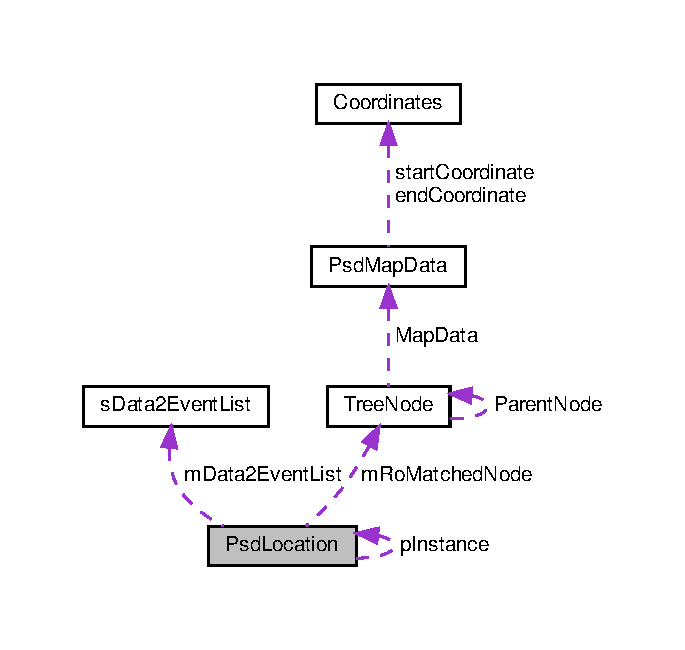
\includegraphics[width=329pt]{class_psd_location__coll__graph}
\end{center}
\end{figure}
\subsection*{Public Member Functions}
\begin{DoxyCompactItemize}
\item 
void \hyperlink{class_psd_location_adf19a491291327b33c1101deb91fe64f}{get\+Diagnotics\+Parameter} ()
\begin{DoxyCompactList}\small\item\em Get the Diagnotics Parameter object. \end{DoxyCompactList}\item 
void \hyperlink{class_psd_location_a4ea349a64cd856f29a26d93f520fc38f}{init\+Psd\+Data} ()
\begin{DoxyCompactList}\small\item\em Initialice Psd relative Data. \end{DoxyCompactList}\item 
void \hyperlink{class_psd_location_a99798cafd2c4257230d9b74215325da0}{create\+Decoder\+Thread} ()
\begin{DoxyCompactList}\small\item\em Create a Decoder Thread object. \end{DoxyCompactList}\item 
void \hyperlink{class_psd_location_a5a7754d385e2b97c9b1e154e02dc0686}{create\+Map\+Thread} ()
\begin{DoxyCompactList}\small\item\em Create a Map Thread object. \end{DoxyCompactList}\item 
\hyperlink{_psd_location_8h_a61af0449f917913c902b37ed397eb350}{Data2\+Event\+List} \hyperlink{class_psd_location_a5bb3ffaeee69beeece9175c0b8bdf491}{get\+Psd\+Ro\+Location} (\hyperlink{_psd_location_8h_a1e3a92020005d2a81aa50ba5ae9b129c}{Data2\+Location} data2\+Location)
\begin{DoxyCompactList}\small\item\em Get the Psd Ro Location object. \end{DoxyCompactList}\item 
void \hyperlink{class_psd_location_acb88267ba5337c7d06687b3121930bc0}{get\+Event\+Distance} ()
\begin{DoxyCompactList}\small\item\em Get the Event Distance object (reserved for V2I) \end{DoxyCompactList}\item 
bool \hyperlink{class_psd_location_aef776415f675a76e9b4c100534ba8ac5}{get\+Psd\+Available} ()
\begin{DoxyCompactList}\small\item\em Get the Psd Available object (Psd whether available or not) \end{DoxyCompactList}\item 
bool \hyperlink{class_psd_location_a07faf8dd338c17fb33e5978b90938c22}{get\+M\+PP} (uint8\+\_\+t Known\+Id)
\begin{DoxyCompactList}\small\item\em Using Ro matched predictive segment\+Id to judge Ro whether is driving on the mpp segment of HV or not. \end{DoxyCompactList}\item 
bool \hyperlink{class_psd_location_a8ff8c5e7cf8057f083f0a1d05fe49d56}{Ro\+Match\+Segment} (\hyperlink{_geometric_calc_8h_aabfa1dd0400b274a48b4a45afbee0af4}{Position3D} Ro\+Point)
\begin{DoxyCompactList}\small\item\em Ro match Segment. \end{DoxyCompactList}\item 
\hyperlink{_psd_message_decoder_8h_a4f9adeb93dfc3dac7961fa97e890b1a5}{Road\+Segment\+Class} \hyperlink{class_psd_location_a49111bfc564db23a9c64612d285ff4bc}{calc\+Road\+Segment\+Class} ()
\begin{DoxyCompactList}\small\item\em Hv\textquotesingle{}s Road Class. \end{DoxyCompactList}\item 
\hyperlink{_psd_location_8h_abcb85fd51379afdf750bdda1dec9174c}{Relative\+Position} \hyperlink{class_psd_location_a3b1402df4271f1470603a82a4fe03b68}{calc\+Relative\+Position} (\hyperlink{_psd_location_8h_a1e3a92020005d2a81aa50ba5ae9b129c}{Data2\+Location} data2\+Location)
\begin{DoxyCompactList}\small\item\em Ro Relative Position to Hv. \end{DoxyCompactList}\item 
\hyperlink{_psd_location_8h_ae65d9d286580719610837075ffad7232}{Realative\+Direction} \hyperlink{class_psd_location_afb451818c3fd9ff5e260270365bf165f}{calc\+Relative\+Direction} (\hyperlink{_psd_location_8h_a1e3a92020005d2a81aa50ba5ae9b129c}{Data2\+Location} data2\+Location)
\begin{DoxyCompactList}\small\item\em Ro Relative Direction to Hv. \end{DoxyCompactList}\item 
\hyperlink{_psd_location_8h_ad3abb902810ad80bbc508a024f5af264}{Relevancy\+Check} \hyperlink{class_psd_location_a9f1a98a1ba23af93df973502332cf10f}{calc\+Rv\+Relevancy} (\hyperlink{_psd_location_8h_a1e3a92020005d2a81aa50ba5ae9b129c}{Data2\+Location} data2\+Location)
\begin{DoxyCompactList}\small\item\em Ro Relevancy to Hv. \end{DoxyCompactList}\item 
float\+\_\+t \hyperlink{class_psd_location_a8b78f66d995b0d621ddb4ed760e1e6a7}{calc\+Distance\+To\+Event} (\hyperlink{_psd_location_8h_a1e3a92020005d2a81aa50ba5ae9b129c}{Data2\+Location} data2\+Location)
\begin{DoxyCompactList}\small\item\em real road distance between Hv and Ro \end{DoxyCompactList}\item 
float\+\_\+t \hyperlink{class_psd_location_a3e8f14fdfe1e6d1495902d265ad6ea93}{calc\+Hv\+Dis2\+Intersection} ()
\begin{DoxyCompactList}\small\item\em D\+T\+IP Hv Distance to Intersection. \end{DoxyCompactList}\item 
float\+\_\+t \hyperlink{class_psd_location_ae9cfb75671bc47a49d167ff8d7d5093c}{calc\+Ro\+Dis2\+Intersection} (\hyperlink{_psd_location_8h_a1e3a92020005d2a81aa50ba5ae9b129c}{Data2\+Location} data2\+Location)
\begin{DoxyCompactList}\small\item\em D\+T\+IP Rv Distance to Intersection. \end{DoxyCompactList}\item 
float\+\_\+t \hyperlink{class_psd_location_a672da471bdc922005cfe26bfaa4315f8}{accumulate\+Childs\+Length} (struct \hyperlink{struct_tree_node}{Tree\+Node} $\ast$Node)
\begin{DoxyCompactList}\small\item\em Accumulate childnodes\textquotesingle{}s pre\+Segment\+Length. \end{DoxyCompactList}\item 
\hyperlink{class_psd_location_a6d89a3bd03a7fe9af26fc08d446bfd24}{Psd\+Location} ()
\begin{DoxyCompactList}\small\item\em Construct a new \hyperlink{class_psd_location}{Psd\+Location} object. \end{DoxyCompactList}\item 
\hyperlink{class_psd_location_ad8df0c3ca51c9df077060c1f8209d977}{$\sim$\+Psd\+Location} ()
\begin{DoxyCompactList}\small\item\em Destroy the \hyperlink{class_psd_location}{Psd\+Location} object. \end{DoxyCompactList}\end{DoxyCompactItemize}
\subsection*{Static Public Member Functions}
\begin{DoxyCompactItemize}
\item 
static \hyperlink{class_psd_location}{Psd\+Location} $\ast$ \hyperlink{class_psd_location_a0ec04eadcec725922d8413aa59d3cb07}{get\+Instance} ()
\begin{DoxyCompactList}\small\item\em Get the Instance object. \end{DoxyCompactList}\end{DoxyCompactItemize}
\subsection*{Public Attributes}
\begin{DoxyCompactItemize}
\item 
pthread\+\_\+t \hyperlink{class_psd_location_a5d7bd3fa135b850706b5e84ae7030e42}{decoder\+Thread}
\item 
pthread\+\_\+t \hyperlink{class_psd_location_a27cc6052f8ad1d5275665eeffcf4e27a}{map\+Thread}
\item 
uint8\+\_\+t \hyperlink{class_psd_location_a58e1c30caca2156e789630b0daf02119}{m\+Ro\+Matched\+Seg\+Id}
\item 
struct \hyperlink{struct_tree_node}{Tree\+Node} $\ast$ \hyperlink{class_psd_location_ab7c279e371a3c0769393213a100b2f97}{m\+Ro\+Matched\+Node}
\item 
\hyperlink{_psd_location_8h_a61af0449f917913c902b37ed397eb350}{Data2\+Event\+List} \hyperlink{class_psd_location_aed2837439f815776affee635d3cb5e51}{m\+Data2\+Event\+List}
\item 
bool \hyperlink{class_psd_location_a7a61732e0ce265903e9b361afac2bcea}{m\+Is\+Match}
\end{DoxyCompactItemize}
\subsection*{Static Public Attributes}
\begin{DoxyCompactItemize}
\item 
static \hyperlink{class_psd_location}{Psd\+Location} $\ast$ \hyperlink{class_psd_location_a65504484bcffebd2f8a95cf7d5b26f2d}{p\+Instance} = N\+U\+LL
\end{DoxyCompactItemize}


\subsection{Detailed Description}
$<$ p\+\_\+\+Stationary\+Threshold 

\subsection{Constructor \& Destructor Documentation}
\mbox{\Hypertarget{class_psd_location_a6d89a3bd03a7fe9af26fc08d446bfd24}\label{class_psd_location_a6d89a3bd03a7fe9af26fc08d446bfd24}} 
\index{Psd\+Location@{Psd\+Location}!Psd\+Location@{Psd\+Location}}
\index{Psd\+Location@{Psd\+Location}!Psd\+Location@{Psd\+Location}}
\subsubsection{\texorpdfstring{Psd\+Location()}{PsdLocation()}}
{\footnotesize\ttfamily Psd\+Location\+::\+Psd\+Location (\begin{DoxyParamCaption}{ }\end{DoxyParamCaption})}



Construct a new \hyperlink{class_psd_location}{Psd\+Location} object. 

\mbox{\Hypertarget{class_psd_location_ad8df0c3ca51c9df077060c1f8209d977}\label{class_psd_location_ad8df0c3ca51c9df077060c1f8209d977}} 
\index{Psd\+Location@{Psd\+Location}!````~Psd\+Location@{$\sim$\+Psd\+Location}}
\index{````~Psd\+Location@{$\sim$\+Psd\+Location}!Psd\+Location@{Psd\+Location}}
\subsubsection{\texorpdfstring{$\sim$\+Psd\+Location()}{~PsdLocation()}}
{\footnotesize\ttfamily Psd\+Location\+::$\sim$\+Psd\+Location (\begin{DoxyParamCaption}{ }\end{DoxyParamCaption})}



Destroy the \hyperlink{class_psd_location}{Psd\+Location} object. 



\subsection{Member Function Documentation}
\mbox{\Hypertarget{class_psd_location_a672da471bdc922005cfe26bfaa4315f8}\label{class_psd_location_a672da471bdc922005cfe26bfaa4315f8}} 
\index{Psd\+Location@{Psd\+Location}!accumulate\+Childs\+Length@{accumulate\+Childs\+Length}}
\index{accumulate\+Childs\+Length@{accumulate\+Childs\+Length}!Psd\+Location@{Psd\+Location}}
\subsubsection{\texorpdfstring{accumulate\+Childs\+Length()}{accumulateChildsLength()}}
{\footnotesize\ttfamily float\+\_\+t Psd\+Location\+::accumulate\+Childs\+Length (\begin{DoxyParamCaption}\item[{struct \hyperlink{struct_tree_node}{Tree\+Node} $\ast$}]{Node }\end{DoxyParamCaption})}



Accumulate childnodes\textquotesingle{}s pre\+Segment\+Length. 


\begin{DoxyParams}{Parameters}
{\em Node} & \\
\hline
\end{DoxyParams}
\begin{DoxyReturn}{Returns}
float\+\_\+t (unit\+: meter, accuracy\+: float) 
\end{DoxyReturn}
\mbox{\Hypertarget{class_psd_location_a8b78f66d995b0d621ddb4ed760e1e6a7}\label{class_psd_location_a8b78f66d995b0d621ddb4ed760e1e6a7}} 
\index{Psd\+Location@{Psd\+Location}!calc\+Distance\+To\+Event@{calc\+Distance\+To\+Event}}
\index{calc\+Distance\+To\+Event@{calc\+Distance\+To\+Event}!Psd\+Location@{Psd\+Location}}
\subsubsection{\texorpdfstring{calc\+Distance\+To\+Event()}{calcDistanceToEvent()}}
{\footnotesize\ttfamily float\+\_\+t Psd\+Location\+::calc\+Distance\+To\+Event (\begin{DoxyParamCaption}\item[{\hyperlink{_psd_location_8h_a1e3a92020005d2a81aa50ba5ae9b129c}{Data2\+Location}}]{data2\+Location }\end{DoxyParamCaption})}



real road distance between Hv and Ro 


\begin{DoxyParams}{Parameters}
{\em data2\+Location} & \\
\hline
\end{DoxyParams}
\begin{DoxyReturn}{Returns}
float\+\_\+t (unit\+: meter, accuracy\+: float) 
\end{DoxyReturn}
\mbox{\Hypertarget{class_psd_location_a3e8f14fdfe1e6d1495902d265ad6ea93}\label{class_psd_location_a3e8f14fdfe1e6d1495902d265ad6ea93}} 
\index{Psd\+Location@{Psd\+Location}!calc\+Hv\+Dis2\+Intersection@{calc\+Hv\+Dis2\+Intersection}}
\index{calc\+Hv\+Dis2\+Intersection@{calc\+Hv\+Dis2\+Intersection}!Psd\+Location@{Psd\+Location}}
\subsubsection{\texorpdfstring{calc\+Hv\+Dis2\+Intersection()}{calcHvDis2Intersection()}}
{\footnotesize\ttfamily float\+\_\+t Psd\+Location\+::calc\+Hv\+Dis2\+Intersection (\begin{DoxyParamCaption}{ }\end{DoxyParamCaption})}



D\+T\+IP Hv Distance to Intersection. 

\begin{DoxyReturn}{Returns}
float\+\_\+t (unit\+: meter, accuracy\+: float) 
\end{DoxyReturn}
\mbox{\Hypertarget{class_psd_location_afb451818c3fd9ff5e260270365bf165f}\label{class_psd_location_afb451818c3fd9ff5e260270365bf165f}} 
\index{Psd\+Location@{Psd\+Location}!calc\+Relative\+Direction@{calc\+Relative\+Direction}}
\index{calc\+Relative\+Direction@{calc\+Relative\+Direction}!Psd\+Location@{Psd\+Location}}
\subsubsection{\texorpdfstring{calc\+Relative\+Direction()}{calcRelativeDirection()}}
{\footnotesize\ttfamily \hyperlink{_psd_location_8h_ae65d9d286580719610837075ffad7232}{Realative\+Direction} Psd\+Location\+::calc\+Relative\+Direction (\begin{DoxyParamCaption}\item[{\hyperlink{_psd_location_8h_a1e3a92020005d2a81aa50ba5ae9b129c}{Data2\+Location}}]{data2\+Location }\end{DoxyParamCaption})}



Ro Relative Direction to Hv. 


\begin{DoxyParams}{Parameters}
{\em data2\+Location} & \\
\hline
\end{DoxyParams}
\begin{DoxyReturn}{Returns}
Realative\+Direction 
\end{DoxyReturn}
\mbox{\Hypertarget{class_psd_location_a3b1402df4271f1470603a82a4fe03b68}\label{class_psd_location_a3b1402df4271f1470603a82a4fe03b68}} 
\index{Psd\+Location@{Psd\+Location}!calc\+Relative\+Position@{calc\+Relative\+Position}}
\index{calc\+Relative\+Position@{calc\+Relative\+Position}!Psd\+Location@{Psd\+Location}}
\subsubsection{\texorpdfstring{calc\+Relative\+Position()}{calcRelativePosition()}}
{\footnotesize\ttfamily \hyperlink{_psd_location_8h_abcb85fd51379afdf750bdda1dec9174c}{Relative\+Position} Psd\+Location\+::calc\+Relative\+Position (\begin{DoxyParamCaption}\item[{\hyperlink{_psd_location_8h_a1e3a92020005d2a81aa50ba5ae9b129c}{Data2\+Location}}]{data2\+Location }\end{DoxyParamCaption})}



Ro Relative Position to Hv. 


\begin{DoxyParams}{Parameters}
{\em data2\+Location} & \\
\hline
\end{DoxyParams}
\begin{DoxyReturn}{Returns}
Relative\+Position 
\end{DoxyReturn}
\mbox{\Hypertarget{class_psd_location_a49111bfc564db23a9c64612d285ff4bc}\label{class_psd_location_a49111bfc564db23a9c64612d285ff4bc}} 
\index{Psd\+Location@{Psd\+Location}!calc\+Road\+Segment\+Class@{calc\+Road\+Segment\+Class}}
\index{calc\+Road\+Segment\+Class@{calc\+Road\+Segment\+Class}!Psd\+Location@{Psd\+Location}}
\subsubsection{\texorpdfstring{calc\+Road\+Segment\+Class()}{calcRoadSegmentClass()}}
{\footnotesize\ttfamily \hyperlink{_psd_message_decoder_8h_a4f9adeb93dfc3dac7961fa97e890b1a5}{Road\+Segment\+Class} Psd\+Location\+::calc\+Road\+Segment\+Class (\begin{DoxyParamCaption}{ }\end{DoxyParamCaption})}



Hv\textquotesingle{}s Road Class. 

\begin{DoxyReturn}{Returns}
Road\+Segment\+Class 
\end{DoxyReturn}
\mbox{\Hypertarget{class_psd_location_ae9cfb75671bc47a49d167ff8d7d5093c}\label{class_psd_location_ae9cfb75671bc47a49d167ff8d7d5093c}} 
\index{Psd\+Location@{Psd\+Location}!calc\+Ro\+Dis2\+Intersection@{calc\+Ro\+Dis2\+Intersection}}
\index{calc\+Ro\+Dis2\+Intersection@{calc\+Ro\+Dis2\+Intersection}!Psd\+Location@{Psd\+Location}}
\subsubsection{\texorpdfstring{calc\+Ro\+Dis2\+Intersection()}{calcRoDis2Intersection()}}
{\footnotesize\ttfamily float\+\_\+t Psd\+Location\+::calc\+Ro\+Dis2\+Intersection (\begin{DoxyParamCaption}\item[{\hyperlink{_psd_location_8h_a1e3a92020005d2a81aa50ba5ae9b129c}{Data2\+Location}}]{data2\+Location }\end{DoxyParamCaption})}



D\+T\+IP Rv Distance to Intersection. 


\begin{DoxyParams}{Parameters}
{\em data2\+Location} & \\
\hline
\end{DoxyParams}
\begin{DoxyReturn}{Returns}
float\+\_\+t (unit\+: meter, accuracy\+: float) 
\end{DoxyReturn}
\mbox{\Hypertarget{class_psd_location_a9f1a98a1ba23af93df973502332cf10f}\label{class_psd_location_a9f1a98a1ba23af93df973502332cf10f}} 
\index{Psd\+Location@{Psd\+Location}!calc\+Rv\+Relevancy@{calc\+Rv\+Relevancy}}
\index{calc\+Rv\+Relevancy@{calc\+Rv\+Relevancy}!Psd\+Location@{Psd\+Location}}
\subsubsection{\texorpdfstring{calc\+Rv\+Relevancy()}{calcRvRelevancy()}}
{\footnotesize\ttfamily \hyperlink{_psd_location_8h_ad3abb902810ad80bbc508a024f5af264}{Relevancy\+Check} Psd\+Location\+::calc\+Rv\+Relevancy (\begin{DoxyParamCaption}\item[{\hyperlink{_psd_location_8h_a1e3a92020005d2a81aa50ba5ae9b129c}{Data2\+Location}}]{data2\+Location }\end{DoxyParamCaption})}



Ro Relevancy to Hv. 

\begin{DoxyReturn}{Returns}
Relevancy\+Check 
\end{DoxyReturn}
\mbox{\Hypertarget{class_psd_location_a99798cafd2c4257230d9b74215325da0}\label{class_psd_location_a99798cafd2c4257230d9b74215325da0}} 
\index{Psd\+Location@{Psd\+Location}!create\+Decoder\+Thread@{create\+Decoder\+Thread}}
\index{create\+Decoder\+Thread@{create\+Decoder\+Thread}!Psd\+Location@{Psd\+Location}}
\subsubsection{\texorpdfstring{create\+Decoder\+Thread()}{createDecoderThread()}}
{\footnotesize\ttfamily void Psd\+Location\+::create\+Decoder\+Thread (\begin{DoxyParamCaption}{ }\end{DoxyParamCaption})}



Create a Decoder Thread object. 

\mbox{\Hypertarget{class_psd_location_a5a7754d385e2b97c9b1e154e02dc0686}\label{class_psd_location_a5a7754d385e2b97c9b1e154e02dc0686}} 
\index{Psd\+Location@{Psd\+Location}!create\+Map\+Thread@{create\+Map\+Thread}}
\index{create\+Map\+Thread@{create\+Map\+Thread}!Psd\+Location@{Psd\+Location}}
\subsubsection{\texorpdfstring{create\+Map\+Thread()}{createMapThread()}}
{\footnotesize\ttfamily void Psd\+Location\+::create\+Map\+Thread (\begin{DoxyParamCaption}{ }\end{DoxyParamCaption})}



Create a Map Thread object. 

\mbox{\Hypertarget{class_psd_location_adf19a491291327b33c1101deb91fe64f}\label{class_psd_location_adf19a491291327b33c1101deb91fe64f}} 
\index{Psd\+Location@{Psd\+Location}!get\+Diagnotics\+Parameter@{get\+Diagnotics\+Parameter}}
\index{get\+Diagnotics\+Parameter@{get\+Diagnotics\+Parameter}!Psd\+Location@{Psd\+Location}}
\subsubsection{\texorpdfstring{get\+Diagnotics\+Parameter()}{getDiagnoticsParameter()}}
{\footnotesize\ttfamily void Psd\+Location\+::get\+Diagnotics\+Parameter (\begin{DoxyParamCaption}{ }\end{DoxyParamCaption})}



Get the Diagnotics Parameter object. 

$<$ Ro whether matched on HV\textquotesingle{}s segments, default value == false \mbox{\Hypertarget{class_psd_location_acb88267ba5337c7d06687b3121930bc0}\label{class_psd_location_acb88267ba5337c7d06687b3121930bc0}} 
\index{Psd\+Location@{Psd\+Location}!get\+Event\+Distance@{get\+Event\+Distance}}
\index{get\+Event\+Distance@{get\+Event\+Distance}!Psd\+Location@{Psd\+Location}}
\subsubsection{\texorpdfstring{get\+Event\+Distance()}{getEventDistance()}}
{\footnotesize\ttfamily void Psd\+Location\+::get\+Event\+Distance (\begin{DoxyParamCaption}{ }\end{DoxyParamCaption})}



Get the Event Distance object (reserved for V2I) 

\mbox{\Hypertarget{class_psd_location_a0ec04eadcec725922d8413aa59d3cb07}\label{class_psd_location_a0ec04eadcec725922d8413aa59d3cb07}} 
\index{Psd\+Location@{Psd\+Location}!get\+Instance@{get\+Instance}}
\index{get\+Instance@{get\+Instance}!Psd\+Location@{Psd\+Location}}
\subsubsection{\texorpdfstring{get\+Instance()}{getInstance()}}
{\footnotesize\ttfamily \hyperlink{class_psd_location}{Psd\+Location} $\ast$ Psd\+Location\+::get\+Instance (\begin{DoxyParamCaption}{ }\end{DoxyParamCaption})\hspace{0.3cm}{\ttfamily [static]}}



Get the Instance object. 

\begin{DoxyReturn}{Returns}
Psd\+Location$\ast$ 
\end{DoxyReturn}
\mbox{\Hypertarget{class_psd_location_a07faf8dd338c17fb33e5978b90938c22}\label{class_psd_location_a07faf8dd338c17fb33e5978b90938c22}} 
\index{Psd\+Location@{Psd\+Location}!get\+M\+PP@{get\+M\+PP}}
\index{get\+M\+PP@{get\+M\+PP}!Psd\+Location@{Psd\+Location}}
\subsubsection{\texorpdfstring{get\+M\+P\+P()}{getMPP()}}
{\footnotesize\ttfamily bool Psd\+Location\+::get\+M\+PP (\begin{DoxyParamCaption}\item[{uint8\+\_\+t}]{Known\+Id }\end{DoxyParamCaption})}



Using Ro matched predictive segment\+Id to judge Ro whether is driving on the mpp segment of HV or not. 


\begin{DoxyParams}{Parameters}
{\em Known\+Id} & \\
\hline
\end{DoxyParams}
\begin{DoxyReturn}{Returns}
true 

false 
\end{DoxyReturn}
\mbox{\Hypertarget{class_psd_location_aef776415f675a76e9b4c100534ba8ac5}\label{class_psd_location_aef776415f675a76e9b4c100534ba8ac5}} 
\index{Psd\+Location@{Psd\+Location}!get\+Psd\+Available@{get\+Psd\+Available}}
\index{get\+Psd\+Available@{get\+Psd\+Available}!Psd\+Location@{Psd\+Location}}
\subsubsection{\texorpdfstring{get\+Psd\+Available()}{getPsdAvailable()}}
{\footnotesize\ttfamily bool Psd\+Location\+::get\+Psd\+Available (\begin{DoxyParamCaption}{ }\end{DoxyParamCaption})}



Get the Psd Available object (Psd whether available or not) 

\begin{DoxyReturn}{Returns}
true (Psd is available) 

false (Psd is not available) 
\end{DoxyReturn}
\mbox{\Hypertarget{class_psd_location_a5bb3ffaeee69beeece9175c0b8bdf491}\label{class_psd_location_a5bb3ffaeee69beeece9175c0b8bdf491}} 
\index{Psd\+Location@{Psd\+Location}!get\+Psd\+Ro\+Location@{get\+Psd\+Ro\+Location}}
\index{get\+Psd\+Ro\+Location@{get\+Psd\+Ro\+Location}!Psd\+Location@{Psd\+Location}}
\subsubsection{\texorpdfstring{get\+Psd\+Ro\+Location()}{getPsdRoLocation()}}
{\footnotesize\ttfamily \hyperlink{_psd_location_8h_a61af0449f917913c902b37ed397eb350}{Data2\+Event\+List} Psd\+Location\+::get\+Psd\+Ro\+Location (\begin{DoxyParamCaption}\item[{\hyperlink{_psd_location_8h_a1e3a92020005d2a81aa50ba5ae9b129c}{Data2\+Location}}]{data2\+Location }\end{DoxyParamCaption})}



Get the Psd Ro Location object. 


\begin{DoxyParams}{Parameters}
{\em data2\+Location} & \\
\hline
\end{DoxyParams}
\begin{DoxyReturn}{Returns}
Data2\+Event\+List 
\end{DoxyReturn}
\mbox{\Hypertarget{class_psd_location_a4ea349a64cd856f29a26d93f520fc38f}\label{class_psd_location_a4ea349a64cd856f29a26d93f520fc38f}} 
\index{Psd\+Location@{Psd\+Location}!init\+Psd\+Data@{init\+Psd\+Data}}
\index{init\+Psd\+Data@{init\+Psd\+Data}!Psd\+Location@{Psd\+Location}}
\subsubsection{\texorpdfstring{init\+Psd\+Data()}{initPsdData()}}
{\footnotesize\ttfamily void Psd\+Location\+::init\+Psd\+Data (\begin{DoxyParamCaption}{ }\end{DoxyParamCaption})}



Initialice Psd relative Data. 

\mbox{\Hypertarget{class_psd_location_a8ff8c5e7cf8057f083f0a1d05fe49d56}\label{class_psd_location_a8ff8c5e7cf8057f083f0a1d05fe49d56}} 
\index{Psd\+Location@{Psd\+Location}!Ro\+Match\+Segment@{Ro\+Match\+Segment}}
\index{Ro\+Match\+Segment@{Ro\+Match\+Segment}!Psd\+Location@{Psd\+Location}}
\subsubsection{\texorpdfstring{Ro\+Match\+Segment()}{RoMatchSegment()}}
{\footnotesize\ttfamily bool Psd\+Location\+::\+Ro\+Match\+Segment (\begin{DoxyParamCaption}\item[{\hyperlink{_geometric_calc_8h_aabfa1dd0400b274a48b4a45afbee0af4}{Position3D}}]{Ro\+Point }\end{DoxyParamCaption})}



Ro match Segment. 


\begin{DoxyParams}{Parameters}
{\em Ro\+Point} & \\
\hline
\end{DoxyParams}
\begin{DoxyReturn}{Returns}
true (Ro matched one segment) 

false (Ro not matched one segment) 
\end{DoxyReturn}


\subsection{Member Data Documentation}
\mbox{\Hypertarget{class_psd_location_a5d7bd3fa135b850706b5e84ae7030e42}\label{class_psd_location_a5d7bd3fa135b850706b5e84ae7030e42}} 
\index{Psd\+Location@{Psd\+Location}!decoder\+Thread@{decoder\+Thread}}
\index{decoder\+Thread@{decoder\+Thread}!Psd\+Location@{Psd\+Location}}
\subsubsection{\texorpdfstring{decoder\+Thread}{decoderThread}}
{\footnotesize\ttfamily pthread\+\_\+t Psd\+Location\+::decoder\+Thread}

\mbox{\Hypertarget{class_psd_location_a27cc6052f8ad1d5275665eeffcf4e27a}\label{class_psd_location_a27cc6052f8ad1d5275665eeffcf4e27a}} 
\index{Psd\+Location@{Psd\+Location}!map\+Thread@{map\+Thread}}
\index{map\+Thread@{map\+Thread}!Psd\+Location@{Psd\+Location}}
\subsubsection{\texorpdfstring{map\+Thread}{mapThread}}
{\footnotesize\ttfamily pthread\+\_\+t Psd\+Location\+::map\+Thread}

$<$ decoder\+Thread\textquotesingle{}s Id \mbox{\Hypertarget{class_psd_location_aed2837439f815776affee635d3cb5e51}\label{class_psd_location_aed2837439f815776affee635d3cb5e51}} 
\index{Psd\+Location@{Psd\+Location}!m\+Data2\+Event\+List@{m\+Data2\+Event\+List}}
\index{m\+Data2\+Event\+List@{m\+Data2\+Event\+List}!Psd\+Location@{Psd\+Location}}
\subsubsection{\texorpdfstring{m\+Data2\+Event\+List}{mData2EventList}}
{\footnotesize\ttfamily \hyperlink{_psd_location_8h_a61af0449f917913c902b37ed397eb350}{Data2\+Event\+List} Psd\+Location\+::m\+Data2\+Event\+List}

$<$ Ro Matched Segment Node \mbox{\Hypertarget{class_psd_location_a7a61732e0ce265903e9b361afac2bcea}\label{class_psd_location_a7a61732e0ce265903e9b361afac2bcea}} 
\index{Psd\+Location@{Psd\+Location}!m\+Is\+Match@{m\+Is\+Match}}
\index{m\+Is\+Match@{m\+Is\+Match}!Psd\+Location@{Psd\+Location}}
\subsubsection{\texorpdfstring{m\+Is\+Match}{mIsMatch}}
{\footnotesize\ttfamily bool Psd\+Location\+::m\+Is\+Match}

$<$ Data return to Event\+List \mbox{\Hypertarget{class_psd_location_ab7c279e371a3c0769393213a100b2f97}\label{class_psd_location_ab7c279e371a3c0769393213a100b2f97}} 
\index{Psd\+Location@{Psd\+Location}!m\+Ro\+Matched\+Node@{m\+Ro\+Matched\+Node}}
\index{m\+Ro\+Matched\+Node@{m\+Ro\+Matched\+Node}!Psd\+Location@{Psd\+Location}}
\subsubsection{\texorpdfstring{m\+Ro\+Matched\+Node}{mRoMatchedNode}}
{\footnotesize\ttfamily struct \hyperlink{struct_tree_node}{Tree\+Node}$\ast$ Psd\+Location\+::m\+Ro\+Matched\+Node}

$<$ Ro Matched Segment Id \mbox{\Hypertarget{class_psd_location_a58e1c30caca2156e789630b0daf02119}\label{class_psd_location_a58e1c30caca2156e789630b0daf02119}} 
\index{Psd\+Location@{Psd\+Location}!m\+Ro\+Matched\+Seg\+Id@{m\+Ro\+Matched\+Seg\+Id}}
\index{m\+Ro\+Matched\+Seg\+Id@{m\+Ro\+Matched\+Seg\+Id}!Psd\+Location@{Psd\+Location}}
\subsubsection{\texorpdfstring{m\+Ro\+Matched\+Seg\+Id}{mRoMatchedSegId}}
{\footnotesize\ttfamily uint8\+\_\+t Psd\+Location\+::m\+Ro\+Matched\+Seg\+Id}

$<$ map\+Thread\textquotesingle{}s Id \mbox{\Hypertarget{class_psd_location_a65504484bcffebd2f8a95cf7d5b26f2d}\label{class_psd_location_a65504484bcffebd2f8a95cf7d5b26f2d}} 
\index{Psd\+Location@{Psd\+Location}!p\+Instance@{p\+Instance}}
\index{p\+Instance@{p\+Instance}!Psd\+Location@{Psd\+Location}}
\subsubsection{\texorpdfstring{p\+Instance}{pInstance}}
{\footnotesize\ttfamily \hyperlink{class_psd_location}{Psd\+Location} $\ast$ Psd\+Location\+::p\+Instance = N\+U\+LL\hspace{0.3cm}{\ttfamily [static]}}

A pointer used to return the object of the class of \hyperlink{class_psd_location}{Psd\+Location} 

The documentation for this class was generated from the following files\+:\begin{DoxyCompactItemize}
\item 
src/\hyperlink{_psd_location_8h}{Psd\+Location.\+h}\item 
src/\hyperlink{_psd_location_8cpp}{Psd\+Location.\+cpp}\end{DoxyCompactItemize}

\hypertarget{class_psd_map}{}\section{Psd\+Map Class Reference}
\label{class_psd_map}\index{Psd\+Map@{Psd\+Map}}


{\ttfamily \#include $<$Psd\+Map.\+h$>$}



Collaboration diagram for Psd\+Map\+:\nopagebreak
\begin{figure}[H]
\begin{center}
\leavevmode
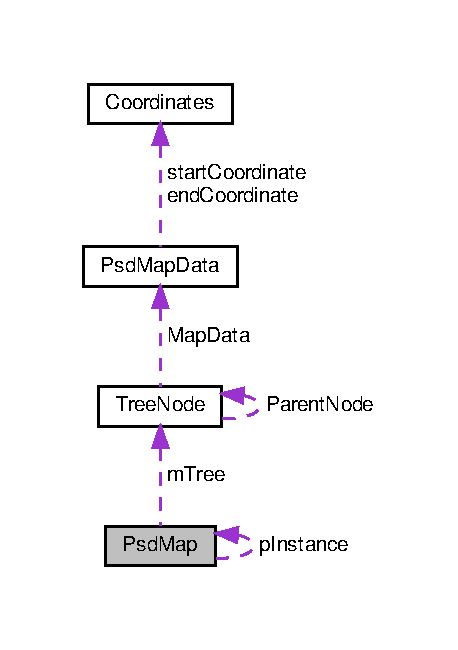
\includegraphics[width=220pt]{class_psd_map__coll__graph}
\end{center}
\end{figure}
\subsection*{Public Member Functions}
\begin{DoxyCompactItemize}
\item 
struct \hyperlink{struct_psd_map_data}{Psd\+Map\+Data} $\ast$ \hyperlink{class_psd_map_a5544295bf3b6f659f10a85cb30c6eef2}{cur\+Id\+Is\+In\+List} ()
\begin{DoxyCompactList}\small\item\em Find Cur\+Segment\+Id whether in list or not. \end{DoxyCompactList}\item 
void \hyperlink{class_psd_map_a0b9829cd0b350a6de1150aaaabd567d4}{map\+Create} ()
\begin{DoxyCompactList}\small\item\em Start triggering create map action. \end{DoxyCompactList}\item 
void \hyperlink{class_psd_map_a325207cab7b23d6880a1690b24700b0b}{map\+Update} ()
\begin{DoxyCompactList}\small\item\em Start triggering update map(the tree) action. \end{DoxyCompactList}\item 
void \hyperlink{class_psd_map_a835d6753d2aecbae14115eacf2502028}{map\+Clear} (struct \hyperlink{struct_tree_node}{Tree\+Node} $\ast$Node)
\begin{DoxyCompactList}\small\item\em Start triggering clear map action. \end{DoxyCompactList}\item 
void \hyperlink{class_psd_map_a7a2135f3db362df35b71fd1a12cac6c3}{insert\+Node\+In\+Tree} ()
\begin{DoxyCompactList}\small\item\em Insert v\+Psd\+Map\textquotesingle{}s data element in m\+Tree. \end{DoxyCompactList}\item 
void \hyperlink{class_psd_map_ac9d868bc2459c1c403c9e5e3e2bb719a}{insert\+Node} (struct \hyperlink{struct_tree_node}{Tree\+Node} $\ast$Node)
\begin{DoxyCompactList}\small\item\em Insert recursively HV\textquotesingle{}s parent, root, childs or child\textquotesingle{}s childs node. \end{DoxyCompactList}\item 
struct \hyperlink{struct_tree_node}{Tree\+Node} $\ast$ \hyperlink{class_psd_map_a4413fa2f7b4dbc83449f184c6b4963cc}{create\+Node} ()
\begin{DoxyCompactList}\small\item\em Create a Node object. \end{DoxyCompactList}\item 
void \hyperlink{class_psd_map_ade677b7a2b308a4c5ce99f343ddc56ff}{update\+Root\+Node} ()
\begin{DoxyCompactList}\small\item\em Start triggering update root(m\+Tree) action. \end{DoxyCompactList}\item 
void \hyperlink{class_psd_map_a3129a5bf0d09334c47ee35a291ee688c}{update\+Child\+Node} ()
\begin{DoxyCompactList}\small\item\em Delete sub\+Tree (update new\+Parent, new\+Current, new\+Childs) \end{DoxyCompactList}\item 
void \hyperlink{class_psd_map_a1ed126a63203198d3aeca3ccef1f4577}{clear\+Node\+Out\+Tree} (struct \hyperlink{struct_tree_node}{Tree\+Node} $\ast$Node)
\begin{DoxyCompactList}\small\item\em Clearing all nodes of m\+Tree actually. \end{DoxyCompactList}\item 
struct \hyperlink{struct_tree_node}{Tree\+Node} $\ast$ \hyperlink{class_psd_map_a2f5e7823124673a335e20ee0e9821836}{delete\+Old\+Root} ()
\begin{DoxyCompactList}\small\item\em Delete old root. \end{DoxyCompactList}\item 
void \hyperlink{class_psd_map_a2309336d5a1a083f2d715a9dc520575d}{delete\+Sub\+Tree} (struct \hyperlink{struct_tree_node}{Tree\+Node} $\ast$Node)
\begin{DoxyCompactList}\small\item\em Delete sub tree. \end{DoxyCompactList}\item 
struct \hyperlink{struct_tree_node}{Tree\+Node} $\ast$ \hyperlink{class_psd_map_aec8b191b16852e62c4234dfba7885aa0}{find\+Node\+By\+Id} (struct \hyperlink{struct_tree_node}{Tree\+Node} $\ast$Node, uint8\+\_\+t Known\+Id)
\begin{DoxyCompactList}\small\item\em Find in m\+Tree by the known id. \end{DoxyCompactList}\item 
struct \hyperlink{struct_psd_map_data}{Psd\+Map\+Data} \hyperlink{class_psd_map_a32a4312f48a064153216831d5b0beb41}{calc\+Coordinate} (struct \hyperlink{struct_tree_node}{Tree\+Node} $\ast$Node)
\begin{DoxyCompactList}\small\item\em Calculate coordinate distinguish between straight path and curved line. \end{DoxyCompactList}\item 
\hyperlink{_psd_message_decoder_8h_a7d8466510c49a8035fcf35b2949bea5a}{t\+Offset} \hyperlink{class_psd_map_ac7db4ce816867efd9074a54a99b7d046}{calc\+Curve\+X\+Y\+Offset} (double S, double A0, double A1, double delta\+Branch\+Angle\+Rad)
\begin{DoxyCompactList}\small\item\em Calculate X Y offsset in curve case. \end{DoxyCompactList}\item 
\hyperlink{_psd_message_decoder_8h_a7d8466510c49a8035fcf35b2949bea5a}{t\+Offset} \hyperlink{class_psd_map_a804df58155e626d0a6309fad2d7c52b9}{calc\+Straight\+X\+Y\+Offset} (double Length, double Branch\+Angle)
\begin{DoxyCompactList}\small\item\em Calculate X Y offsset in straight path case. \end{DoxyCompactList}\item 
\hyperlink{_psd_message_decoder_8h_a7d8466510c49a8035fcf35b2949bea5a}{t\+Offset} \hyperlink{class_psd_map_a2319f4363ead5ff44b847570509f2fca}{calc\+Heading\+XY} (double Heading, double distanceX, double distanceY)
\begin{DoxyCompactList}\small\item\em Calculate horizontal and orthogonal distance. \end{DoxyCompactList}\item 
struct \hyperlink{struct_tree_node}{Tree\+Node} $\ast$ \hyperlink{class_psd_map_a69a64b755dbacc77737bf6e05686c001}{get\+Tree} ()
\begin{DoxyCompactList}\small\item\em Get the Tree object. \end{DoxyCompactList}\item 
void \hyperlink{class_psd_map_a56643c65f1e5d4af827259354572d57a}{set\+Tree} (struct \hyperlink{struct_tree_node}{Tree\+Node} $\ast$Node)
\begin{DoxyCompactList}\small\item\em Set the Tree object. \end{DoxyCompactList}\item 
bool \hyperlink{class_psd_map_a411472433a3037b0245e9c9f699672b4}{get\+Map\+Mutex\+Status} ()
\begin{DoxyCompactList}\small\item\em Get the Map Mutex Status object. \end{DoxyCompactList}\item 
void \hyperlink{class_psd_map_ac9eeeec55caef16f27da6bd14da5f3a4}{set\+Map\+Mutex\+Status} (bool Mutex\+Status)
\begin{DoxyCompactList}\small\item\em Set the Map Mutex Status object (for gtest branch coverage) \end{DoxyCompactList}\item 
\hyperlink{class_psd_map_a0f0d7e4f35c32b85cc855b375bfdf6f1}{Psd\+Map} ()
\begin{DoxyCompactList}\small\item\em Construct a new \hyperlink{class_psd_map}{Psd\+Map} object. \end{DoxyCompactList}\item 
\hyperlink{class_psd_map_a027edc72c34c1d7845385bb57bff0956}{$\sim$\+Psd\+Map} ()
\begin{DoxyCompactList}\small\item\em Destroy the \hyperlink{class_psd_map}{Psd\+Map} object. \end{DoxyCompactList}\end{DoxyCompactItemize}
\subsection*{Static Public Member Functions}
\begin{DoxyCompactItemize}
\item 
static \hyperlink{class_psd_map}{Psd\+Map} $\ast$ \hyperlink{class_psd_map_a559bfdc80678bf39ebcf0d351d002838}{get\+Instance} ()
\begin{DoxyCompactList}\small\item\em Get the Instance object. \end{DoxyCompactList}\end{DoxyCompactItemize}
\subsection*{Public Attributes}
\begin{DoxyCompactItemize}
\item 
struct \hyperlink{struct_tree_node}{Tree\+Node} $\ast$ \hyperlink{class_psd_map_a906a31bbf47593efd39648627ec84d04}{m\+Tree}
\item 
pthread\+\_\+mutex\+\_\+t \hyperlink{class_psd_map_a8fbc224227e28dec675589a701b9d8ad}{map\+Thread\+Mutex}
\item 
bool \hyperlink{class_psd_map_affea202c3988b6f45fe19c8669121816}{m\+Map\+Mutex\+Is\+Locked}
\end{DoxyCompactItemize}
\subsection*{Static Public Attributes}
\begin{DoxyCompactItemize}
\item 
static \hyperlink{class_psd_map}{Psd\+Map} $\ast$ \hyperlink{class_psd_map_a9d0824203886b61bfea66530e401dcd1}{p\+Instance} = N\+U\+LL
\end{DoxyCompactItemize}


\subsection{Constructor \& Destructor Documentation}
\mbox{\Hypertarget{class_psd_map_a0f0d7e4f35c32b85cc855b375bfdf6f1}\label{class_psd_map_a0f0d7e4f35c32b85cc855b375bfdf6f1}} 
\index{Psd\+Map@{Psd\+Map}!Psd\+Map@{Psd\+Map}}
\index{Psd\+Map@{Psd\+Map}!Psd\+Map@{Psd\+Map}}
\subsubsection{\texorpdfstring{Psd\+Map()}{PsdMap()}}
{\footnotesize\ttfamily Psd\+Map\+::\+Psd\+Map (\begin{DoxyParamCaption}{ }\end{DoxyParamCaption})}



Construct a new \hyperlink{class_psd_map}{Psd\+Map} object. 

\mbox{\Hypertarget{class_psd_map_a027edc72c34c1d7845385bb57bff0956}\label{class_psd_map_a027edc72c34c1d7845385bb57bff0956}} 
\index{Psd\+Map@{Psd\+Map}!````~Psd\+Map@{$\sim$\+Psd\+Map}}
\index{````~Psd\+Map@{$\sim$\+Psd\+Map}!Psd\+Map@{Psd\+Map}}
\subsubsection{\texorpdfstring{$\sim$\+Psd\+Map()}{~PsdMap()}}
{\footnotesize\ttfamily Psd\+Map\+::$\sim$\+Psd\+Map (\begin{DoxyParamCaption}{ }\end{DoxyParamCaption})}



Destroy the \hyperlink{class_psd_map}{Psd\+Map} object. 



\subsection{Member Function Documentation}
\mbox{\Hypertarget{class_psd_map_a32a4312f48a064153216831d5b0beb41}\label{class_psd_map_a32a4312f48a064153216831d5b0beb41}} 
\index{Psd\+Map@{Psd\+Map}!calc\+Coordinate@{calc\+Coordinate}}
\index{calc\+Coordinate@{calc\+Coordinate}!Psd\+Map@{Psd\+Map}}
\subsubsection{\texorpdfstring{calc\+Coordinate()}{calcCoordinate()}}
{\footnotesize\ttfamily struct \hyperlink{struct_psd_map_data}{Psd\+Map\+Data} Psd\+Map\+::calc\+Coordinate (\begin{DoxyParamCaption}\item[{struct \hyperlink{struct_tree_node}{Tree\+Node} $\ast$}]{Node }\end{DoxyParamCaption})}



Calculate coordinate distinguish between straight path and curved line. 


\begin{DoxyParams}{Parameters}
{\em Node} & (can represent any node) \\
\hline
\end{DoxyParams}
\begin{DoxyReturn}{Returns}
struct \hyperlink{struct_psd_map_data}{Psd\+Map\+Data} (data fields for each node) 
\end{DoxyReturn}
\mbox{\Hypertarget{class_psd_map_ac7db4ce816867efd9074a54a99b7d046}\label{class_psd_map_ac7db4ce816867efd9074a54a99b7d046}} 
\index{Psd\+Map@{Psd\+Map}!calc\+Curve\+X\+Y\+Offset@{calc\+Curve\+X\+Y\+Offset}}
\index{calc\+Curve\+X\+Y\+Offset@{calc\+Curve\+X\+Y\+Offset}!Psd\+Map@{Psd\+Map}}
\subsubsection{\texorpdfstring{calc\+Curve\+X\+Y\+Offset()}{calcCurveXYOffset()}}
{\footnotesize\ttfamily \hyperlink{_psd_message_decoder_8h_a7d8466510c49a8035fcf35b2949bea5a}{t\+Offset} Psd\+Map\+::calc\+Curve\+X\+Y\+Offset (\begin{DoxyParamCaption}\item[{double}]{S,  }\item[{double}]{A0,  }\item[{double}]{A1,  }\item[{double}]{delta\+Branch\+Angle\+Rad }\end{DoxyParamCaption})}



Calculate X Y offsset in curve case. 


\begin{DoxyParams}{Parameters}
{\em S} & (actual arc length, the length of a curve segment) \\
\hline
{\em A0} & (clothoide parameter, starting value for each sampling point) \\
\hline
{\em A1} & (clothoide parameter, sample the value of the next sampling point) \\
\hline
{\em delta\+Branch\+Angle\+Rad} & (branching angle relative to the previous position) \\
\hline
\end{DoxyParams}
\begin{DoxyReturn}{Returns}
t\+Offset (vertical offset x and horizontal offset y after rotating Branch\+Angle) 
\end{DoxyReturn}
\mbox{\Hypertarget{class_psd_map_a2319f4363ead5ff44b847570509f2fca}\label{class_psd_map_a2319f4363ead5ff44b847570509f2fca}} 
\index{Psd\+Map@{Psd\+Map}!calc\+Heading\+XY@{calc\+Heading\+XY}}
\index{calc\+Heading\+XY@{calc\+Heading\+XY}!Psd\+Map@{Psd\+Map}}
\subsubsection{\texorpdfstring{calc\+Heading\+X\+Y()}{calcHeadingXY()}}
{\footnotesize\ttfamily \hyperlink{_psd_message_decoder_8h_a7d8466510c49a8035fcf35b2949bea5a}{t\+Offset} Psd\+Map\+::calc\+Heading\+XY (\begin{DoxyParamCaption}\item[{double}]{Heading,  }\item[{double}]{distanceX,  }\item[{double}]{distanceY }\end{DoxyParamCaption})}



Calculate horizontal and orthogonal distance. 


\begin{DoxyParams}{Parameters}
{\em Heading} & (from HV) \\
\hline
{\em distanceX} & (x-\/axis before rotation) \\
\hline
{\em distanceY} & (y-\/axis before rotation) \\
\hline
\end{DoxyParams}
\begin{DoxyReturn}{Returns}
t\+Offset (vertical offset x and horizontal offset y after rotation) 
\end{DoxyReturn}
\mbox{\Hypertarget{class_psd_map_a804df58155e626d0a6309fad2d7c52b9}\label{class_psd_map_a804df58155e626d0a6309fad2d7c52b9}} 
\index{Psd\+Map@{Psd\+Map}!calc\+Straight\+X\+Y\+Offset@{calc\+Straight\+X\+Y\+Offset}}
\index{calc\+Straight\+X\+Y\+Offset@{calc\+Straight\+X\+Y\+Offset}!Psd\+Map@{Psd\+Map}}
\subsubsection{\texorpdfstring{calc\+Straight\+X\+Y\+Offset()}{calcStraightXYOffset()}}
{\footnotesize\ttfamily \hyperlink{_psd_message_decoder_8h_a7d8466510c49a8035fcf35b2949bea5a}{t\+Offset} Psd\+Map\+::calc\+Straight\+X\+Y\+Offset (\begin{DoxyParamCaption}\item[{double}]{Length,  }\item[{double}]{Branch\+Angle }\end{DoxyParamCaption})}



Calculate X Y offsset in straight path case. 


\begin{DoxyParams}{Parameters}
{\em Length} & (actual length) \\
\hline
{\em Branch\+Angle} & (branching angle relative to the previous position) \\
\hline
\end{DoxyParams}
\begin{DoxyReturn}{Returns}
t\+Offset (vertical offset x and horizontal offset y after rotating Branch\+Angle) 
\end{DoxyReturn}
\mbox{\Hypertarget{class_psd_map_a1ed126a63203198d3aeca3ccef1f4577}\label{class_psd_map_a1ed126a63203198d3aeca3ccef1f4577}} 
\index{Psd\+Map@{Psd\+Map}!clear\+Node\+Out\+Tree@{clear\+Node\+Out\+Tree}}
\index{clear\+Node\+Out\+Tree@{clear\+Node\+Out\+Tree}!Psd\+Map@{Psd\+Map}}
\subsubsection{\texorpdfstring{clear\+Node\+Out\+Tree()}{clearNodeOutTree()}}
{\footnotesize\ttfamily void Psd\+Map\+::clear\+Node\+Out\+Tree (\begin{DoxyParamCaption}\item[{struct \hyperlink{struct_tree_node}{Tree\+Node} $\ast$}]{Node }\end{DoxyParamCaption})}



Clearing all nodes of m\+Tree actually. 


\begin{DoxyParams}{Parameters}
{\em Node} & (can represent any node) \\
\hline
\end{DoxyParams}
\mbox{\Hypertarget{class_psd_map_a4413fa2f7b4dbc83449f184c6b4963cc}\label{class_psd_map_a4413fa2f7b4dbc83449f184c6b4963cc}} 
\index{Psd\+Map@{Psd\+Map}!create\+Node@{create\+Node}}
\index{create\+Node@{create\+Node}!Psd\+Map@{Psd\+Map}}
\subsubsection{\texorpdfstring{create\+Node()}{createNode()}}
{\footnotesize\ttfamily struct \hyperlink{struct_tree_node}{Tree\+Node} $\ast$ Psd\+Map\+::create\+Node (\begin{DoxyParamCaption}{ }\end{DoxyParamCaption})}



Create a Node object. 

\begin{DoxyReturn}{Returns}
struct Tree\+Node$\ast$ 
\end{DoxyReturn}
\mbox{\Hypertarget{class_psd_map_a5544295bf3b6f659f10a85cb30c6eef2}\label{class_psd_map_a5544295bf3b6f659f10a85cb30c6eef2}} 
\index{Psd\+Map@{Psd\+Map}!cur\+Id\+Is\+In\+List@{cur\+Id\+Is\+In\+List}}
\index{cur\+Id\+Is\+In\+List@{cur\+Id\+Is\+In\+List}!Psd\+Map@{Psd\+Map}}
\subsubsection{\texorpdfstring{cur\+Id\+Is\+In\+List()}{curIdIsInList()}}
{\footnotesize\ttfamily struct \hyperlink{struct_psd_map_data}{Psd\+Map\+Data} $\ast$ Psd\+Map\+::cur\+Id\+Is\+In\+List (\begin{DoxyParamCaption}{ }\end{DoxyParamCaption})}



Find Cur\+Segment\+Id whether in list or not. 

$<$ the status of Mutex whether is locked or not \begin{DoxyReturn}{Returns}
struct Psd\+Map\+Data$\ast$ (the location of the list where HV is located, otherwise return N\+U\+LL) 
\end{DoxyReturn}
\mbox{\Hypertarget{class_psd_map_a2f5e7823124673a335e20ee0e9821836}\label{class_psd_map_a2f5e7823124673a335e20ee0e9821836}} 
\index{Psd\+Map@{Psd\+Map}!delete\+Old\+Root@{delete\+Old\+Root}}
\index{delete\+Old\+Root@{delete\+Old\+Root}!Psd\+Map@{Psd\+Map}}
\subsubsection{\texorpdfstring{delete\+Old\+Root()}{deleteOldRoot()}}
{\footnotesize\ttfamily struct \hyperlink{struct_tree_node}{Tree\+Node} $\ast$ Psd\+Map\+::delete\+Old\+Root (\begin{DoxyParamCaption}{ }\end{DoxyParamCaption})}



Delete old root. 

\begin{DoxyReturn}{Returns}
struct Tree\+Node$\ast$ (returns new root if m\+Tree is not N\+U\+LL, otherwise returns N\+U\+LL) 
\end{DoxyReturn}
\mbox{\Hypertarget{class_psd_map_a2309336d5a1a083f2d715a9dc520575d}\label{class_psd_map_a2309336d5a1a083f2d715a9dc520575d}} 
\index{Psd\+Map@{Psd\+Map}!delete\+Sub\+Tree@{delete\+Sub\+Tree}}
\index{delete\+Sub\+Tree@{delete\+Sub\+Tree}!Psd\+Map@{Psd\+Map}}
\subsubsection{\texorpdfstring{delete\+Sub\+Tree()}{deleteSubTree()}}
{\footnotesize\ttfamily void Psd\+Map\+::delete\+Sub\+Tree (\begin{DoxyParamCaption}\item[{struct \hyperlink{struct_tree_node}{Tree\+Node} $\ast$}]{Node }\end{DoxyParamCaption})}



Delete sub tree. 


\begin{DoxyParams}{Parameters}
{\em Node} & (can represent any node) \\
\hline
\end{DoxyParams}
\mbox{\Hypertarget{class_psd_map_aec8b191b16852e62c4234dfba7885aa0}\label{class_psd_map_aec8b191b16852e62c4234dfba7885aa0}} 
\index{Psd\+Map@{Psd\+Map}!find\+Node\+By\+Id@{find\+Node\+By\+Id}}
\index{find\+Node\+By\+Id@{find\+Node\+By\+Id}!Psd\+Map@{Psd\+Map}}
\subsubsection{\texorpdfstring{find\+Node\+By\+Id()}{findNodeById()}}
{\footnotesize\ttfamily struct \hyperlink{struct_tree_node}{Tree\+Node} $\ast$ Psd\+Map\+::find\+Node\+By\+Id (\begin{DoxyParamCaption}\item[{struct \hyperlink{struct_tree_node}{Tree\+Node} $\ast$}]{Node,  }\item[{uint8\+\_\+t}]{Known\+Id }\end{DoxyParamCaption})}



Find in m\+Tree by the known id. 


\begin{DoxyParams}{Parameters}
{\em Node} & (can represent any node) \\
\hline
{\em Known\+Id} & \\
\hline
\end{DoxyParams}
\begin{DoxyReturn}{Returns}
struct Tree\+Node$\ast$ (returns the corresponding node in the m\+Tree if found, otherwise returns N\+U\+LL) 
\end{DoxyReturn}
\mbox{\Hypertarget{class_psd_map_a559bfdc80678bf39ebcf0d351d002838}\label{class_psd_map_a559bfdc80678bf39ebcf0d351d002838}} 
\index{Psd\+Map@{Psd\+Map}!get\+Instance@{get\+Instance}}
\index{get\+Instance@{get\+Instance}!Psd\+Map@{Psd\+Map}}
\subsubsection{\texorpdfstring{get\+Instance()}{getInstance()}}
{\footnotesize\ttfamily \hyperlink{class_psd_map}{Psd\+Map} $\ast$ Psd\+Map\+::get\+Instance (\begin{DoxyParamCaption}{ }\end{DoxyParamCaption})\hspace{0.3cm}{\ttfamily [static]}}



Get the Instance object. 

\begin{DoxyReturn}{Returns}
Psd\+Map$\ast$ (\hyperlink{class_psd_map}{Psd\+Map}) 
\end{DoxyReturn}
\mbox{\Hypertarget{class_psd_map_a411472433a3037b0245e9c9f699672b4}\label{class_psd_map_a411472433a3037b0245e9c9f699672b4}} 
\index{Psd\+Map@{Psd\+Map}!get\+Map\+Mutex\+Status@{get\+Map\+Mutex\+Status}}
\index{get\+Map\+Mutex\+Status@{get\+Map\+Mutex\+Status}!Psd\+Map@{Psd\+Map}}
\subsubsection{\texorpdfstring{get\+Map\+Mutex\+Status()}{getMapMutexStatus()}}
{\footnotesize\ttfamily bool Psd\+Map\+::get\+Map\+Mutex\+Status (\begin{DoxyParamCaption}{ }\end{DoxyParamCaption})}



Get the Map Mutex Status object. 

\begin{DoxyReturn}{Returns}
true (map\+Thread\+Mutex is locked) 

false (map\+Thread\+Mutex is unlocked) 
\end{DoxyReturn}
\mbox{\Hypertarget{class_psd_map_a69a64b755dbacc77737bf6e05686c001}\label{class_psd_map_a69a64b755dbacc77737bf6e05686c001}} 
\index{Psd\+Map@{Psd\+Map}!get\+Tree@{get\+Tree}}
\index{get\+Tree@{get\+Tree}!Psd\+Map@{Psd\+Map}}
\subsubsection{\texorpdfstring{get\+Tree()}{getTree()}}
{\footnotesize\ttfamily struct \hyperlink{struct_tree_node}{Tree\+Node} $\ast$ Psd\+Map\+::get\+Tree (\begin{DoxyParamCaption}{ }\end{DoxyParamCaption})}



Get the Tree object. 

\begin{DoxyReturn}{Returns}
struct Tree\+Node$\ast$ 
\end{DoxyReturn}
\mbox{\Hypertarget{class_psd_map_ac9d868bc2459c1c403c9e5e3e2bb719a}\label{class_psd_map_ac9d868bc2459c1c403c9e5e3e2bb719a}} 
\index{Psd\+Map@{Psd\+Map}!insert\+Node@{insert\+Node}}
\index{insert\+Node@{insert\+Node}!Psd\+Map@{Psd\+Map}}
\subsubsection{\texorpdfstring{insert\+Node()}{insertNode()}}
{\footnotesize\ttfamily void Psd\+Map\+::insert\+Node (\begin{DoxyParamCaption}\item[{struct \hyperlink{struct_tree_node}{Tree\+Node} $\ast$}]{Node }\end{DoxyParamCaption})}



Insert recursively HV\textquotesingle{}s parent, root, childs or child\textquotesingle{}s childs node. 


\begin{DoxyParams}{Parameters}
{\em Node} & (can represent any node) \\
\hline
\end{DoxyParams}
\mbox{\Hypertarget{class_psd_map_a7a2135f3db362df35b71fd1a12cac6c3}\label{class_psd_map_a7a2135f3db362df35b71fd1a12cac6c3}} 
\index{Psd\+Map@{Psd\+Map}!insert\+Node\+In\+Tree@{insert\+Node\+In\+Tree}}
\index{insert\+Node\+In\+Tree@{insert\+Node\+In\+Tree}!Psd\+Map@{Psd\+Map}}
\subsubsection{\texorpdfstring{insert\+Node\+In\+Tree()}{insertNodeInTree()}}
{\footnotesize\ttfamily void Psd\+Map\+::insert\+Node\+In\+Tree (\begin{DoxyParamCaption}{ }\end{DoxyParamCaption})}



Insert v\+Psd\+Map\textquotesingle{}s data element in m\+Tree. 

\mbox{\Hypertarget{class_psd_map_a835d6753d2aecbae14115eacf2502028}\label{class_psd_map_a835d6753d2aecbae14115eacf2502028}} 
\index{Psd\+Map@{Psd\+Map}!map\+Clear@{map\+Clear}}
\index{map\+Clear@{map\+Clear}!Psd\+Map@{Psd\+Map}}
\subsubsection{\texorpdfstring{map\+Clear()}{mapClear()}}
{\footnotesize\ttfamily void Psd\+Map\+::map\+Clear (\begin{DoxyParamCaption}\item[{struct \hyperlink{struct_tree_node}{Tree\+Node} $\ast$}]{Node }\end{DoxyParamCaption})}



Start triggering clear map action. 


\begin{DoxyParams}{Parameters}
{\em Node} & (start clearing from m\+Tree) \\
\hline
\end{DoxyParams}
\mbox{\Hypertarget{class_psd_map_a0b9829cd0b350a6de1150aaaabd567d4}\label{class_psd_map_a0b9829cd0b350a6de1150aaaabd567d4}} 
\index{Psd\+Map@{Psd\+Map}!map\+Create@{map\+Create}}
\index{map\+Create@{map\+Create}!Psd\+Map@{Psd\+Map}}
\subsubsection{\texorpdfstring{map\+Create()}{mapCreate()}}
{\footnotesize\ttfamily void Psd\+Map\+::map\+Create (\begin{DoxyParamCaption}{ }\end{DoxyParamCaption})}



Start triggering create map action. 

\mbox{\Hypertarget{class_psd_map_a325207cab7b23d6880a1690b24700b0b}\label{class_psd_map_a325207cab7b23d6880a1690b24700b0b}} 
\index{Psd\+Map@{Psd\+Map}!map\+Update@{map\+Update}}
\index{map\+Update@{map\+Update}!Psd\+Map@{Psd\+Map}}
\subsubsection{\texorpdfstring{map\+Update()}{mapUpdate()}}
{\footnotesize\ttfamily void Psd\+Map\+::map\+Update (\begin{DoxyParamCaption}{ }\end{DoxyParamCaption})}



Start triggering update map(the tree) action. 

\mbox{\Hypertarget{class_psd_map_ac9eeeec55caef16f27da6bd14da5f3a4}\label{class_psd_map_ac9eeeec55caef16f27da6bd14da5f3a4}} 
\index{Psd\+Map@{Psd\+Map}!set\+Map\+Mutex\+Status@{set\+Map\+Mutex\+Status}}
\index{set\+Map\+Mutex\+Status@{set\+Map\+Mutex\+Status}!Psd\+Map@{Psd\+Map}}
\subsubsection{\texorpdfstring{set\+Map\+Mutex\+Status()}{setMapMutexStatus()}}
{\footnotesize\ttfamily void Psd\+Map\+::set\+Map\+Mutex\+Status (\begin{DoxyParamCaption}\item[{bool}]{Mutex\+Status }\end{DoxyParamCaption})}



Set the Map Mutex Status object (for gtest branch coverage) 


\begin{DoxyParams}{Parameters}
{\em Mutex\+Status} & \\
\hline
\end{DoxyParams}
\mbox{\Hypertarget{class_psd_map_a56643c65f1e5d4af827259354572d57a}\label{class_psd_map_a56643c65f1e5d4af827259354572d57a}} 
\index{Psd\+Map@{Psd\+Map}!set\+Tree@{set\+Tree}}
\index{set\+Tree@{set\+Tree}!Psd\+Map@{Psd\+Map}}
\subsubsection{\texorpdfstring{set\+Tree()}{setTree()}}
{\footnotesize\ttfamily void Psd\+Map\+::set\+Tree (\begin{DoxyParamCaption}\item[{struct \hyperlink{struct_tree_node}{Tree\+Node} $\ast$}]{Node }\end{DoxyParamCaption})}



Set the Tree object. 


\begin{DoxyParams}{Parameters}
{\em Node} & (set the Node to m\+Tree) \\
\hline
\end{DoxyParams}
\mbox{\Hypertarget{class_psd_map_a3129a5bf0d09334c47ee35a291ee688c}\label{class_psd_map_a3129a5bf0d09334c47ee35a291ee688c}} 
\index{Psd\+Map@{Psd\+Map}!update\+Child\+Node@{update\+Child\+Node}}
\index{update\+Child\+Node@{update\+Child\+Node}!Psd\+Map@{Psd\+Map}}
\subsubsection{\texorpdfstring{update\+Child\+Node()}{updateChildNode()}}
{\footnotesize\ttfamily void Psd\+Map\+::update\+Child\+Node (\begin{DoxyParamCaption}{ }\end{DoxyParamCaption})}



Delete sub\+Tree (update new\+Parent, new\+Current, new\+Childs) 

\mbox{\Hypertarget{class_psd_map_ade677b7a2b308a4c5ce99f343ddc56ff}\label{class_psd_map_ade677b7a2b308a4c5ce99f343ddc56ff}} 
\index{Psd\+Map@{Psd\+Map}!update\+Root\+Node@{update\+Root\+Node}}
\index{update\+Root\+Node@{update\+Root\+Node}!Psd\+Map@{Psd\+Map}}
\subsubsection{\texorpdfstring{update\+Root\+Node()}{updateRootNode()}}
{\footnotesize\ttfamily void Psd\+Map\+::update\+Root\+Node (\begin{DoxyParamCaption}{ }\end{DoxyParamCaption})}



Start triggering update root(m\+Tree) action. 



\subsection{Member Data Documentation}
\mbox{\Hypertarget{class_psd_map_a8fbc224227e28dec675589a701b9d8ad}\label{class_psd_map_a8fbc224227e28dec675589a701b9d8ad}} 
\index{Psd\+Map@{Psd\+Map}!map\+Thread\+Mutex@{map\+Thread\+Mutex}}
\index{map\+Thread\+Mutex@{map\+Thread\+Mutex}!Psd\+Map@{Psd\+Map}}
\subsubsection{\texorpdfstring{map\+Thread\+Mutex}{mapThreadMutex}}
{\footnotesize\ttfamily pthread\+\_\+mutex\+\_\+t Psd\+Map\+::map\+Thread\+Mutex}

$<$ Root node of segment, representing the root node of the tree \mbox{\Hypertarget{class_psd_map_affea202c3988b6f45fe19c8669121816}\label{class_psd_map_affea202c3988b6f45fe19c8669121816}} 
\index{Psd\+Map@{Psd\+Map}!m\+Map\+Mutex\+Is\+Locked@{m\+Map\+Mutex\+Is\+Locked}}
\index{m\+Map\+Mutex\+Is\+Locked@{m\+Map\+Mutex\+Is\+Locked}!Psd\+Map@{Psd\+Map}}
\subsubsection{\texorpdfstring{m\+Map\+Mutex\+Is\+Locked}{mMapMutexIsLocked}}
{\footnotesize\ttfamily bool Psd\+Map\+::m\+Map\+Mutex\+Is\+Locked}

$<$ Mutex for \hyperlink{class_psd_map}{Psd\+Map} thread \mbox{\Hypertarget{class_psd_map_a906a31bbf47593efd39648627ec84d04}\label{class_psd_map_a906a31bbf47593efd39648627ec84d04}} 
\index{Psd\+Map@{Psd\+Map}!m\+Tree@{m\+Tree}}
\index{m\+Tree@{m\+Tree}!Psd\+Map@{Psd\+Map}}
\subsubsection{\texorpdfstring{m\+Tree}{mTree}}
{\footnotesize\ttfamily struct \hyperlink{struct_tree_node}{Tree\+Node}$\ast$ Psd\+Map\+::m\+Tree}

\mbox{\Hypertarget{class_psd_map_a9d0824203886b61bfea66530e401dcd1}\label{class_psd_map_a9d0824203886b61bfea66530e401dcd1}} 
\index{Psd\+Map@{Psd\+Map}!p\+Instance@{p\+Instance}}
\index{p\+Instance@{p\+Instance}!Psd\+Map@{Psd\+Map}}
\subsubsection{\texorpdfstring{p\+Instance}{pInstance}}
{\footnotesize\ttfamily \hyperlink{class_psd_map}{Psd\+Map} $\ast$ Psd\+Map\+::p\+Instance = N\+U\+LL\hspace{0.3cm}{\ttfamily [static]}}

A pointer used to return the object of the class of \hyperlink{class_psd_map}{Psd\+Map} 

The documentation for this class was generated from the following files\+:\begin{DoxyCompactItemize}
\item 
src/\hyperlink{_psd_map_8h}{Psd\+Map.\+h}\item 
src/\hyperlink{_psd_map_8cpp}{Psd\+Map.\+cpp}\end{DoxyCompactItemize}

\hypertarget{struct_psd_map_data}{}\section{Psd\+Map\+Data Struct Reference}
\label{struct_psd_map_data}\index{Psd\+Map\+Data@{Psd\+Map\+Data}}


{\ttfamily \#include $<$Psd\+Message\+Decoder.\+h$>$}



Collaboration diagram for Psd\+Map\+Data\+:\nopagebreak
\begin{figure}[H]
\begin{center}
\leavevmode
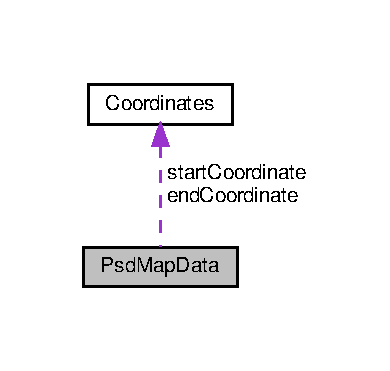
\includegraphics[width=187pt]{struct_psd_map_data__coll__graph}
\end{center}
\end{figure}
\subsection*{Public Attributes}
\begin{DoxyCompactItemize}
\item 
uint8\+\_\+t \hyperlink{struct_psd_map_data_a05964b04396fbe60313638b68146409c}{pre\+Segment\+Id}
\item 
uint8\+\_\+t \hyperlink{struct_psd_map_data_a7f96bd3b8eaffbbfa479fc218951a18e}{prev\+Segment\+Id}
\item 
uint16\+\_\+t \hyperlink{struct_psd_map_data_aff96ab7a862bbb292f8b97891f95cfe5}{pre\+Seg\+Total\+Length}
\item 
\hyperlink{_psd_message_decoder_8h_a39044ce168ac526920bc721a8dc702b9}{Psd04\+Road\+Class} \hyperlink{struct_psd_map_data_ab3d6bede9882ba6c46776e493a8d312e}{psd04\+Road\+Class}
\item 
double \hyperlink{struct_psd_map_data_ab8b6fcfdb85cd9041b4c1d6557b73cf1}{end\+Curvature}
\item 
bool \hyperlink{struct_psd_map_data_ae27e54d6d968caec9488192a5ef020b3}{sign\+End\+Curvature}
\item 
bool \hyperlink{struct_psd_map_data_a7660ef05fe24afd46c2a2588844daf66}{mpp}
\item 
bool \hyperlink{struct_psd_map_data_a733402b0de1cb1d31e433ca7d9da2e99}{sp}
\item 
bool \hyperlink{struct_psd_map_data_adbdd4923256006ea09ea96cdb1e1df21}{segment\+Is\+Complete}
\item 
double \hyperlink{struct_psd_map_data_ae478c00c2ea8dc9b99ed23b4b5327cce}{start\+Curvature}
\item 
bool \hyperlink{struct_psd_map_data_ad888b35e0757aaf8edb6afd246a5ed6f}{sign\+Start\+Curvature}
\item 
bool \hyperlink{struct_psd_map_data_a41ac719f3013692691e22e24329f9725}{branch\+Direction}
\item 
double \hyperlink{struct_psd_map_data_ae032895a5e9238f14ba4a63264c24334}{branch\+Angle}
\item 
double \hyperlink{struct_psd_map_data_a843771a8237479d2fb51be8583e8324c}{accumulate\+Branch\+Angle}
\item 
bool \hyperlink{struct_psd_map_data_ae027448738c569007b8b58951532da4b}{seg\+Is\+In\+Tree}
\item 
\hyperlink{_psd_message_decoder_8h_aa38e8413bd76f11962a364459c725e06}{e\+\_\+\+Node\+Attribute} \hyperlink{struct_psd_map_data_a6112249db6720d9fd94a9a06f5d9b926}{node\+Attribute}
\item 
\hyperlink{_psd_message_decoder_8h_a559ada7297c8c6c2337f9e233e73aeca}{t\+Coordinates} \hyperlink{struct_psd_map_data_ab949d9f64982e7cce89b723c95fe01b5}{start\+Coordinate}
\item 
\hyperlink{_psd_message_decoder_8h_a559ada7297c8c6c2337f9e233e73aeca}{t\+Coordinates} \hyperlink{struct_psd_map_data_a5fb30ffcc95a2d29bad59e04804757d1}{end\+Coordinate}
\item 
std\+::vector$<$ struct \hyperlink{struct_coordinates}{Coordinates} $>$ \hyperlink{struct_psd_map_data_a03b022aae0167ffbdf0827f4850e8641}{v\+Sample\+Coord}
\item 
\hyperlink{_psd_message_decoder_8h_a2ba67cb465ee836b9ce8470f32577f21}{e\+\_\+\+Struct\+Separate} \hyperlink{struct_psd_map_data_a9f19a6ccb1eeced87a174728c3025df2}{struct\+Separate}
\item 
uint8\+\_\+t \hyperlink{struct_psd_map_data_a40e775104152a6ae51fb28cb2fb7d70a}{psd\+Attribut\+Segment\+ID}
\item 
uint8\+\_\+t \hyperlink{struct_psd_map_data_ae34340428af587dcc6c3107c0c6c703a}{psd\+Attribut1\+ID}
\item 
uint8\+\_\+t \hyperlink{struct_psd_map_data_a67a275329ea7f8d998c3913c60f41769}{psd\+Attribut1\+Wert}
\item 
uint8\+\_\+t \hyperlink{struct_psd_map_data_a946e6b08753f7e21f4d2ddb3719edb67}{psd\+Attribut2\+ID}
\item 
uint8\+\_\+t \hyperlink{struct_psd_map_data_acc46644be6b612d7c34c5f335e9dfaea}{psd\+Attribut2\+Wert}
\item 
uint8\+\_\+t \hyperlink{struct_psd_map_data_a0aa192ba15a029361a7594b33ab7a65e}{psd\+Attribut3\+ID}
\item 
uint8\+\_\+t \hyperlink{struct_psd_map_data_a0a61989c2cec9807cdc9e93009fe15ce}{psd\+Attribut3\+Wert}
\item 
uint8\+\_\+t \hyperlink{struct_psd_map_data_a52875b4fa9208f2f25c70c7a046c4b6f}{psd\+Attribut4\+ID}
\item 
uint8\+\_\+t \hyperlink{struct_psd_map_data_ad1eab0140ddd2bd43024b0dd39da204b}{psd\+Attribut4\+Wert}
\item 
uint8\+\_\+t \hyperlink{struct_psd_map_data_aa63a8f91cda7bbcb052d89ab1c790b42}{psd\+Attribut5\+ID}
\item 
uint8\+\_\+t \hyperlink{struct_psd_map_data_aa1f43de18baaddd807e57a2f7eaa4166}{psd\+Attribut5\+Wert}
\end{DoxyCompactItemize}


\subsection{Member Data Documentation}
\mbox{\Hypertarget{struct_psd_map_data_a843771a8237479d2fb51be8583e8324c}\label{struct_psd_map_data_a843771a8237479d2fb51be8583e8324c}} 
\index{Psd\+Map\+Data@{Psd\+Map\+Data}!accumulate\+Branch\+Angle@{accumulate\+Branch\+Angle}}
\index{accumulate\+Branch\+Angle@{accumulate\+Branch\+Angle}!Psd\+Map\+Data@{Psd\+Map\+Data}}
\subsubsection{\texorpdfstring{accumulate\+Branch\+Angle}{accumulateBranchAngle}}
{\footnotesize\ttfamily double Psd\+Map\+Data\+::accumulate\+Branch\+Angle}

\mbox{\Hypertarget{struct_psd_map_data_ae032895a5e9238f14ba4a63264c24334}\label{struct_psd_map_data_ae032895a5e9238f14ba4a63264c24334}} 
\index{Psd\+Map\+Data@{Psd\+Map\+Data}!branch\+Angle@{branch\+Angle}}
\index{branch\+Angle@{branch\+Angle}!Psd\+Map\+Data@{Psd\+Map\+Data}}
\subsubsection{\texorpdfstring{branch\+Angle}{branchAngle}}
{\footnotesize\ttfamily double Psd\+Map\+Data\+::branch\+Angle}

\mbox{\Hypertarget{struct_psd_map_data_a41ac719f3013692691e22e24329f9725}\label{struct_psd_map_data_a41ac719f3013692691e22e24329f9725}} 
\index{Psd\+Map\+Data@{Psd\+Map\+Data}!branch\+Direction@{branch\+Direction}}
\index{branch\+Direction@{branch\+Direction}!Psd\+Map\+Data@{Psd\+Map\+Data}}
\subsubsection{\texorpdfstring{branch\+Direction}{branchDirection}}
{\footnotesize\ttfamily bool Psd\+Map\+Data\+::branch\+Direction}

\mbox{\Hypertarget{struct_psd_map_data_a5fb30ffcc95a2d29bad59e04804757d1}\label{struct_psd_map_data_a5fb30ffcc95a2d29bad59e04804757d1}} 
\index{Psd\+Map\+Data@{Psd\+Map\+Data}!end\+Coordinate@{end\+Coordinate}}
\index{end\+Coordinate@{end\+Coordinate}!Psd\+Map\+Data@{Psd\+Map\+Data}}
\subsubsection{\texorpdfstring{end\+Coordinate}{endCoordinate}}
{\footnotesize\ttfamily \hyperlink{_psd_message_decoder_8h_a559ada7297c8c6c2337f9e233e73aeca}{t\+Coordinates} Psd\+Map\+Data\+::end\+Coordinate}

\mbox{\Hypertarget{struct_psd_map_data_ab8b6fcfdb85cd9041b4c1d6557b73cf1}\label{struct_psd_map_data_ab8b6fcfdb85cd9041b4c1d6557b73cf1}} 
\index{Psd\+Map\+Data@{Psd\+Map\+Data}!end\+Curvature@{end\+Curvature}}
\index{end\+Curvature@{end\+Curvature}!Psd\+Map\+Data@{Psd\+Map\+Data}}
\subsubsection{\texorpdfstring{end\+Curvature}{endCurvature}}
{\footnotesize\ttfamily double Psd\+Map\+Data\+::end\+Curvature}

\mbox{\Hypertarget{struct_psd_map_data_a7660ef05fe24afd46c2a2588844daf66}\label{struct_psd_map_data_a7660ef05fe24afd46c2a2588844daf66}} 
\index{Psd\+Map\+Data@{Psd\+Map\+Data}!mpp@{mpp}}
\index{mpp@{mpp}!Psd\+Map\+Data@{Psd\+Map\+Data}}
\subsubsection{\texorpdfstring{mpp}{mpp}}
{\footnotesize\ttfamily bool Psd\+Map\+Data\+::mpp}

\mbox{\Hypertarget{struct_psd_map_data_a6112249db6720d9fd94a9a06f5d9b926}\label{struct_psd_map_data_a6112249db6720d9fd94a9a06f5d9b926}} 
\index{Psd\+Map\+Data@{Psd\+Map\+Data}!node\+Attribute@{node\+Attribute}}
\index{node\+Attribute@{node\+Attribute}!Psd\+Map\+Data@{Psd\+Map\+Data}}
\subsubsection{\texorpdfstring{node\+Attribute}{nodeAttribute}}
{\footnotesize\ttfamily \hyperlink{_psd_message_decoder_8h_aa38e8413bd76f11962a364459c725e06}{e\+\_\+\+Node\+Attribute} Psd\+Map\+Data\+::node\+Attribute}

\mbox{\Hypertarget{struct_psd_map_data_a05964b04396fbe60313638b68146409c}\label{struct_psd_map_data_a05964b04396fbe60313638b68146409c}} 
\index{Psd\+Map\+Data@{Psd\+Map\+Data}!pre\+Segment\+Id@{pre\+Segment\+Id}}
\index{pre\+Segment\+Id@{pre\+Segment\+Id}!Psd\+Map\+Data@{Psd\+Map\+Data}}
\subsubsection{\texorpdfstring{pre\+Segment\+Id}{preSegmentId}}
{\footnotesize\ttfamily uint8\+\_\+t Psd\+Map\+Data\+::pre\+Segment\+Id}

\mbox{\Hypertarget{struct_psd_map_data_aff96ab7a862bbb292f8b97891f95cfe5}\label{struct_psd_map_data_aff96ab7a862bbb292f8b97891f95cfe5}} 
\index{Psd\+Map\+Data@{Psd\+Map\+Data}!pre\+Seg\+Total\+Length@{pre\+Seg\+Total\+Length}}
\index{pre\+Seg\+Total\+Length@{pre\+Seg\+Total\+Length}!Psd\+Map\+Data@{Psd\+Map\+Data}}
\subsubsection{\texorpdfstring{pre\+Seg\+Total\+Length}{preSegTotalLength}}
{\footnotesize\ttfamily uint16\+\_\+t Psd\+Map\+Data\+::pre\+Seg\+Total\+Length}

\mbox{\Hypertarget{struct_psd_map_data_a7f96bd3b8eaffbbfa479fc218951a18e}\label{struct_psd_map_data_a7f96bd3b8eaffbbfa479fc218951a18e}} 
\index{Psd\+Map\+Data@{Psd\+Map\+Data}!prev\+Segment\+Id@{prev\+Segment\+Id}}
\index{prev\+Segment\+Id@{prev\+Segment\+Id}!Psd\+Map\+Data@{Psd\+Map\+Data}}
\subsubsection{\texorpdfstring{prev\+Segment\+Id}{prevSegmentId}}
{\footnotesize\ttfamily uint8\+\_\+t Psd\+Map\+Data\+::prev\+Segment\+Id}

\mbox{\Hypertarget{struct_psd_map_data_ab3d6bede9882ba6c46776e493a8d312e}\label{struct_psd_map_data_ab3d6bede9882ba6c46776e493a8d312e}} 
\index{Psd\+Map\+Data@{Psd\+Map\+Data}!psd04\+Road\+Class@{psd04\+Road\+Class}}
\index{psd04\+Road\+Class@{psd04\+Road\+Class}!Psd\+Map\+Data@{Psd\+Map\+Data}}
\subsubsection{\texorpdfstring{psd04\+Road\+Class}{psd04RoadClass}}
{\footnotesize\ttfamily \hyperlink{_psd_message_decoder_8h_a39044ce168ac526920bc721a8dc702b9}{Psd04\+Road\+Class} Psd\+Map\+Data\+::psd04\+Road\+Class}

\mbox{\Hypertarget{struct_psd_map_data_ae34340428af587dcc6c3107c0c6c703a}\label{struct_psd_map_data_ae34340428af587dcc6c3107c0c6c703a}} 
\index{Psd\+Map\+Data@{Psd\+Map\+Data}!psd\+Attribut1\+ID@{psd\+Attribut1\+ID}}
\index{psd\+Attribut1\+ID@{psd\+Attribut1\+ID}!Psd\+Map\+Data@{Psd\+Map\+Data}}
\subsubsection{\texorpdfstring{psd\+Attribut1\+ID}{psdAttribut1ID}}
{\footnotesize\ttfamily uint8\+\_\+t Psd\+Map\+Data\+::psd\+Attribut1\+ID}

\mbox{\Hypertarget{struct_psd_map_data_a67a275329ea7f8d998c3913c60f41769}\label{struct_psd_map_data_a67a275329ea7f8d998c3913c60f41769}} 
\index{Psd\+Map\+Data@{Psd\+Map\+Data}!psd\+Attribut1\+Wert@{psd\+Attribut1\+Wert}}
\index{psd\+Attribut1\+Wert@{psd\+Attribut1\+Wert}!Psd\+Map\+Data@{Psd\+Map\+Data}}
\subsubsection{\texorpdfstring{psd\+Attribut1\+Wert}{psdAttribut1Wert}}
{\footnotesize\ttfamily uint8\+\_\+t Psd\+Map\+Data\+::psd\+Attribut1\+Wert}

\mbox{\Hypertarget{struct_psd_map_data_a946e6b08753f7e21f4d2ddb3719edb67}\label{struct_psd_map_data_a946e6b08753f7e21f4d2ddb3719edb67}} 
\index{Psd\+Map\+Data@{Psd\+Map\+Data}!psd\+Attribut2\+ID@{psd\+Attribut2\+ID}}
\index{psd\+Attribut2\+ID@{psd\+Attribut2\+ID}!Psd\+Map\+Data@{Psd\+Map\+Data}}
\subsubsection{\texorpdfstring{psd\+Attribut2\+ID}{psdAttribut2ID}}
{\footnotesize\ttfamily uint8\+\_\+t Psd\+Map\+Data\+::psd\+Attribut2\+ID}

\mbox{\Hypertarget{struct_psd_map_data_acc46644be6b612d7c34c5f335e9dfaea}\label{struct_psd_map_data_acc46644be6b612d7c34c5f335e9dfaea}} 
\index{Psd\+Map\+Data@{Psd\+Map\+Data}!psd\+Attribut2\+Wert@{psd\+Attribut2\+Wert}}
\index{psd\+Attribut2\+Wert@{psd\+Attribut2\+Wert}!Psd\+Map\+Data@{Psd\+Map\+Data}}
\subsubsection{\texorpdfstring{psd\+Attribut2\+Wert}{psdAttribut2Wert}}
{\footnotesize\ttfamily uint8\+\_\+t Psd\+Map\+Data\+::psd\+Attribut2\+Wert}

\mbox{\Hypertarget{struct_psd_map_data_a0aa192ba15a029361a7594b33ab7a65e}\label{struct_psd_map_data_a0aa192ba15a029361a7594b33ab7a65e}} 
\index{Psd\+Map\+Data@{Psd\+Map\+Data}!psd\+Attribut3\+ID@{psd\+Attribut3\+ID}}
\index{psd\+Attribut3\+ID@{psd\+Attribut3\+ID}!Psd\+Map\+Data@{Psd\+Map\+Data}}
\subsubsection{\texorpdfstring{psd\+Attribut3\+ID}{psdAttribut3ID}}
{\footnotesize\ttfamily uint8\+\_\+t Psd\+Map\+Data\+::psd\+Attribut3\+ID}

\mbox{\Hypertarget{struct_psd_map_data_a0a61989c2cec9807cdc9e93009fe15ce}\label{struct_psd_map_data_a0a61989c2cec9807cdc9e93009fe15ce}} 
\index{Psd\+Map\+Data@{Psd\+Map\+Data}!psd\+Attribut3\+Wert@{psd\+Attribut3\+Wert}}
\index{psd\+Attribut3\+Wert@{psd\+Attribut3\+Wert}!Psd\+Map\+Data@{Psd\+Map\+Data}}
\subsubsection{\texorpdfstring{psd\+Attribut3\+Wert}{psdAttribut3Wert}}
{\footnotesize\ttfamily uint8\+\_\+t Psd\+Map\+Data\+::psd\+Attribut3\+Wert}

\mbox{\Hypertarget{struct_psd_map_data_a52875b4fa9208f2f25c70c7a046c4b6f}\label{struct_psd_map_data_a52875b4fa9208f2f25c70c7a046c4b6f}} 
\index{Psd\+Map\+Data@{Psd\+Map\+Data}!psd\+Attribut4\+ID@{psd\+Attribut4\+ID}}
\index{psd\+Attribut4\+ID@{psd\+Attribut4\+ID}!Psd\+Map\+Data@{Psd\+Map\+Data}}
\subsubsection{\texorpdfstring{psd\+Attribut4\+ID}{psdAttribut4ID}}
{\footnotesize\ttfamily uint8\+\_\+t Psd\+Map\+Data\+::psd\+Attribut4\+ID}

\mbox{\Hypertarget{struct_psd_map_data_ad1eab0140ddd2bd43024b0dd39da204b}\label{struct_psd_map_data_ad1eab0140ddd2bd43024b0dd39da204b}} 
\index{Psd\+Map\+Data@{Psd\+Map\+Data}!psd\+Attribut4\+Wert@{psd\+Attribut4\+Wert}}
\index{psd\+Attribut4\+Wert@{psd\+Attribut4\+Wert}!Psd\+Map\+Data@{Psd\+Map\+Data}}
\subsubsection{\texorpdfstring{psd\+Attribut4\+Wert}{psdAttribut4Wert}}
{\footnotesize\ttfamily uint8\+\_\+t Psd\+Map\+Data\+::psd\+Attribut4\+Wert}

\mbox{\Hypertarget{struct_psd_map_data_aa63a8f91cda7bbcb052d89ab1c790b42}\label{struct_psd_map_data_aa63a8f91cda7bbcb052d89ab1c790b42}} 
\index{Psd\+Map\+Data@{Psd\+Map\+Data}!psd\+Attribut5\+ID@{psd\+Attribut5\+ID}}
\index{psd\+Attribut5\+ID@{psd\+Attribut5\+ID}!Psd\+Map\+Data@{Psd\+Map\+Data}}
\subsubsection{\texorpdfstring{psd\+Attribut5\+ID}{psdAttribut5ID}}
{\footnotesize\ttfamily uint8\+\_\+t Psd\+Map\+Data\+::psd\+Attribut5\+ID}

\mbox{\Hypertarget{struct_psd_map_data_aa1f43de18baaddd807e57a2f7eaa4166}\label{struct_psd_map_data_aa1f43de18baaddd807e57a2f7eaa4166}} 
\index{Psd\+Map\+Data@{Psd\+Map\+Data}!psd\+Attribut5\+Wert@{psd\+Attribut5\+Wert}}
\index{psd\+Attribut5\+Wert@{psd\+Attribut5\+Wert}!Psd\+Map\+Data@{Psd\+Map\+Data}}
\subsubsection{\texorpdfstring{psd\+Attribut5\+Wert}{psdAttribut5Wert}}
{\footnotesize\ttfamily uint8\+\_\+t Psd\+Map\+Data\+::psd\+Attribut5\+Wert}

\mbox{\Hypertarget{struct_psd_map_data_a40e775104152a6ae51fb28cb2fb7d70a}\label{struct_psd_map_data_a40e775104152a6ae51fb28cb2fb7d70a}} 
\index{Psd\+Map\+Data@{Psd\+Map\+Data}!psd\+Attribut\+Segment\+ID@{psd\+Attribut\+Segment\+ID}}
\index{psd\+Attribut\+Segment\+ID@{psd\+Attribut\+Segment\+ID}!Psd\+Map\+Data@{Psd\+Map\+Data}}
\subsubsection{\texorpdfstring{psd\+Attribut\+Segment\+ID}{psdAttributSegmentID}}
{\footnotesize\ttfamily uint8\+\_\+t Psd\+Map\+Data\+::psd\+Attribut\+Segment\+ID}

\mbox{\Hypertarget{struct_psd_map_data_ae027448738c569007b8b58951532da4b}\label{struct_psd_map_data_ae027448738c569007b8b58951532da4b}} 
\index{Psd\+Map\+Data@{Psd\+Map\+Data}!seg\+Is\+In\+Tree@{seg\+Is\+In\+Tree}}
\index{seg\+Is\+In\+Tree@{seg\+Is\+In\+Tree}!Psd\+Map\+Data@{Psd\+Map\+Data}}
\subsubsection{\texorpdfstring{seg\+Is\+In\+Tree}{segIsInTree}}
{\footnotesize\ttfamily bool Psd\+Map\+Data\+::seg\+Is\+In\+Tree}

\mbox{\Hypertarget{struct_psd_map_data_adbdd4923256006ea09ea96cdb1e1df21}\label{struct_psd_map_data_adbdd4923256006ea09ea96cdb1e1df21}} 
\index{Psd\+Map\+Data@{Psd\+Map\+Data}!segment\+Is\+Complete@{segment\+Is\+Complete}}
\index{segment\+Is\+Complete@{segment\+Is\+Complete}!Psd\+Map\+Data@{Psd\+Map\+Data}}
\subsubsection{\texorpdfstring{segment\+Is\+Complete}{segmentIsComplete}}
{\footnotesize\ttfamily bool Psd\+Map\+Data\+::segment\+Is\+Complete}

\mbox{\Hypertarget{struct_psd_map_data_ae27e54d6d968caec9488192a5ef020b3}\label{struct_psd_map_data_ae27e54d6d968caec9488192a5ef020b3}} 
\index{Psd\+Map\+Data@{Psd\+Map\+Data}!sign\+End\+Curvature@{sign\+End\+Curvature}}
\index{sign\+End\+Curvature@{sign\+End\+Curvature}!Psd\+Map\+Data@{Psd\+Map\+Data}}
\subsubsection{\texorpdfstring{sign\+End\+Curvature}{signEndCurvature}}
{\footnotesize\ttfamily bool Psd\+Map\+Data\+::sign\+End\+Curvature}

\mbox{\Hypertarget{struct_psd_map_data_ad888b35e0757aaf8edb6afd246a5ed6f}\label{struct_psd_map_data_ad888b35e0757aaf8edb6afd246a5ed6f}} 
\index{Psd\+Map\+Data@{Psd\+Map\+Data}!sign\+Start\+Curvature@{sign\+Start\+Curvature}}
\index{sign\+Start\+Curvature@{sign\+Start\+Curvature}!Psd\+Map\+Data@{Psd\+Map\+Data}}
\subsubsection{\texorpdfstring{sign\+Start\+Curvature}{signStartCurvature}}
{\footnotesize\ttfamily bool Psd\+Map\+Data\+::sign\+Start\+Curvature}

\mbox{\Hypertarget{struct_psd_map_data_a733402b0de1cb1d31e433ca7d9da2e99}\label{struct_psd_map_data_a733402b0de1cb1d31e433ca7d9da2e99}} 
\index{Psd\+Map\+Data@{Psd\+Map\+Data}!sp@{sp}}
\index{sp@{sp}!Psd\+Map\+Data@{Psd\+Map\+Data}}
\subsubsection{\texorpdfstring{sp}{sp}}
{\footnotesize\ttfamily bool Psd\+Map\+Data\+::sp}

\mbox{\Hypertarget{struct_psd_map_data_ab949d9f64982e7cce89b723c95fe01b5}\label{struct_psd_map_data_ab949d9f64982e7cce89b723c95fe01b5}} 
\index{Psd\+Map\+Data@{Psd\+Map\+Data}!start\+Coordinate@{start\+Coordinate}}
\index{start\+Coordinate@{start\+Coordinate}!Psd\+Map\+Data@{Psd\+Map\+Data}}
\subsubsection{\texorpdfstring{start\+Coordinate}{startCoordinate}}
{\footnotesize\ttfamily \hyperlink{_psd_message_decoder_8h_a559ada7297c8c6c2337f9e233e73aeca}{t\+Coordinates} Psd\+Map\+Data\+::start\+Coordinate}

\mbox{\Hypertarget{struct_psd_map_data_ae478c00c2ea8dc9b99ed23b4b5327cce}\label{struct_psd_map_data_ae478c00c2ea8dc9b99ed23b4b5327cce}} 
\index{Psd\+Map\+Data@{Psd\+Map\+Data}!start\+Curvature@{start\+Curvature}}
\index{start\+Curvature@{start\+Curvature}!Psd\+Map\+Data@{Psd\+Map\+Data}}
\subsubsection{\texorpdfstring{start\+Curvature}{startCurvature}}
{\footnotesize\ttfamily double Psd\+Map\+Data\+::start\+Curvature}

\mbox{\Hypertarget{struct_psd_map_data_a9f19a6ccb1eeced87a174728c3025df2}\label{struct_psd_map_data_a9f19a6ccb1eeced87a174728c3025df2}} 
\index{Psd\+Map\+Data@{Psd\+Map\+Data}!struct\+Separate@{struct\+Separate}}
\index{struct\+Separate@{struct\+Separate}!Psd\+Map\+Data@{Psd\+Map\+Data}}
\subsubsection{\texorpdfstring{struct\+Separate}{structSeparate}}
{\footnotesize\ttfamily \hyperlink{_psd_message_decoder_8h_a2ba67cb465ee836b9ce8470f32577f21}{e\+\_\+\+Struct\+Separate} Psd\+Map\+Data\+::struct\+Separate}

\mbox{\Hypertarget{struct_psd_map_data_a03b022aae0167ffbdf0827f4850e8641}\label{struct_psd_map_data_a03b022aae0167ffbdf0827f4850e8641}} 
\index{Psd\+Map\+Data@{Psd\+Map\+Data}!v\+Sample\+Coord@{v\+Sample\+Coord}}
\index{v\+Sample\+Coord@{v\+Sample\+Coord}!Psd\+Map\+Data@{Psd\+Map\+Data}}
\subsubsection{\texorpdfstring{v\+Sample\+Coord}{vSampleCoord}}
{\footnotesize\ttfamily std\+::vector$<$struct \hyperlink{struct_coordinates}{Coordinates}$>$ Psd\+Map\+Data\+::v\+Sample\+Coord}



The documentation for this struct was generated from the following file\+:\begin{DoxyCompactItemize}
\item 
src/\hyperlink{_psd_message_decoder_8h}{Psd\+Message\+Decoder.\+h}\end{DoxyCompactItemize}

\hypertarget{class_psd_message_decoder}{}\section{Psd\+Message\+Decoder Class Reference}
\label{class_psd_message_decoder}\index{Psd\+Message\+Decoder@{Psd\+Message\+Decoder}}


{\ttfamily \#include $<$Psd\+Message\+Decoder.\+h$>$}



Collaboration diagram for Psd\+Message\+Decoder\+:\nopagebreak
\begin{figure}[H]
\begin{center}
\leavevmode
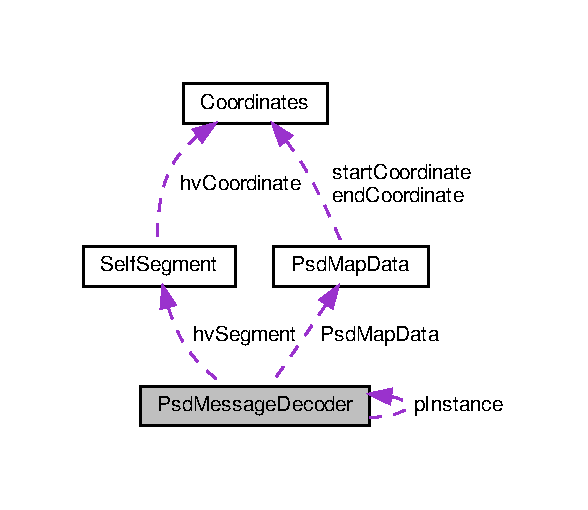
\includegraphics[width=282pt]{class_psd_message_decoder__coll__graph}
\end{center}
\end{figure}
\subsection*{Public Member Functions}
\begin{DoxyCompactItemize}
\item 
void \hyperlink{class_psd_message_decoder_adea08ce30ab67d1a71ab7ea4463ed4a2}{segment\+Manager} (bool Psd\+Usage\+Active)
\begin{DoxyCompactList}\small\item\em Putting \hyperlink{struct_psd_map_data}{Psd\+Map\+Data} into container when Psd\+Usage\+Active is true, clearing the container when Psd\+Usage\+Active is false. \end{DoxyCompactList}\item 
void \hyperlink{class_psd_message_decoder_a34359c377ca6c6940025facd6b177130}{calc\+Psd04\+Data} ()
\begin{DoxyCompactList}\small\item\em Calculate P\+S\+D\+\_\+04 data. \end{DoxyCompactList}\item 
void \hyperlink{class_psd_message_decoder_a88607430974b48dd7379f636f3bb0b35}{convert\+Curvature} ()
\begin{DoxyCompactList}\small\item\em Convert start \&\& end Curvature from uint8\+\_\+t to double type. \end{DoxyCompactList}\item 
void \hyperlink{class_psd_message_decoder_adf3d4c8211c7a08f9de2f74509361ea6}{convert\+Branch\+Angle} ()
\begin{DoxyCompactList}\small\item\em Convert branch\+Angle from uint8\+\_\+t to double type. \end{DoxyCompactList}\item 
void \hyperlink{class_psd_message_decoder_a8fbd5e60c5807f9879de028f4593bbc4}{push\+In\+List} ()
\begin{DoxyCompactList}\small\item\em \hyperlink{struct_psd_map_data}{Psd\+Map\+Data} emplace in container. \end{DoxyCompactList}\item 
void \hyperlink{class_psd_message_decoder_a3f782b96f0fb6f05cd2178c626d7058b}{pop\+Up\+List} (std\+::vector$<$ struct \hyperlink{struct_psd_map_data}{Psd\+Map\+Data} $\ast$$>$\+::iterator position)
\begin{DoxyCompactList}\small\item\em \hyperlink{struct_psd_map_data}{Psd\+Map\+Data} erase out container. \end{DoxyCompactList}\item 
void \hyperlink{class_psd_message_decoder_a1d3d09203c12851fd048e97069bc8d5a}{clear\+List} ()
\begin{DoxyCompactList}\small\item\em Clear the container. \end{DoxyCompactList}\item 
void \hyperlink{class_psd_message_decoder_ab65ca19c37ae0fcf45af498081c80e18}{save\+Attribut\+To\+List} ()
\begin{DoxyCompactList}\small\item\em Check Struct\+Separate info and save in container. \end{DoxyCompactList}\item 
\hyperlink{_psd_message_decoder_8h_a6c858ba8556a68d900d0eca9dc406232}{t\+Self\+Segment} \hyperlink{class_psd_message_decoder_a7d7ee9d6bcaefbb6375cf5ab5b63d232}{get\+Self\+Segment} ()
\begin{DoxyCompactList}\small\item\em Get the Self Segment object. \end{DoxyCompactList}\item 
void \hyperlink{class_psd_message_decoder_ad9dd4ec66688adb0616b97de091aa6e7}{set\+Self\+Segment} (\hyperlink{_psd_message_decoder_8h_a6c858ba8556a68d900d0eca9dc406232}{t\+Self\+Segment} \hyperlink{struct_self_segment}{Self\+Segment})
\begin{DoxyCompactList}\small\item\em Set the Self Segment object. \end{DoxyCompactList}\item 
void \hyperlink{class_psd_message_decoder_a6c92018754baf45e25e682cd153864af}{set\+Psd\+Map\+Data} (\hyperlink{_psd_message_decoder_8h_ad54e183dd7c544312c06d4bd6279ebdc}{t\+Psd\+Map\+Data} psd\+Map\+Data)
\begin{DoxyCompactList}\small\item\em Set the Psd Map Data object. \end{DoxyCompactList}\item 
std\+::vector$<$ struct \hyperlink{struct_psd_map_data}{Psd\+Map\+Data} $\ast$ $>$ \& \hyperlink{class_psd_message_decoder_a9ab6fa68448dff44ad93bcb37a2a9690}{get\+V\+Psd\+Map} ()
\begin{DoxyCompactList}\small\item\em Get the container with \hyperlink{struct_psd_map_data}{Psd\+Map\+Data}. \end{DoxyCompactList}\item 
\hyperlink{class_psd_message_decoder_ac767a18e119cad2cc3dbfbcac6368af2}{Psd\+Message\+Decoder} ()
\begin{DoxyCompactList}\small\item\em Construct a new \hyperlink{class_psd_message_decoder}{Psd\+Message\+Decoder} object. \end{DoxyCompactList}\item 
\hyperlink{class_psd_message_decoder_a097a557e58d4b9782660aba304cd2bba}{$\sim$\+Psd\+Message\+Decoder} ()
\begin{DoxyCompactList}\small\item\em Destroy the \hyperlink{class_psd_message_decoder}{Psd\+Message\+Decoder} object. \end{DoxyCompactList}\end{DoxyCompactItemize}
\subsection*{Static Public Member Functions}
\begin{DoxyCompactItemize}
\item 
static \hyperlink{class_psd_message_decoder}{Psd\+Message\+Decoder} $\ast$ \hyperlink{class_psd_message_decoder_a544f32786ee3bf1b7747fd1b82604ccf}{get\+Instance} ()
\begin{DoxyCompactList}\small\item\em Get the Instance object. \end{DoxyCompactList}\end{DoxyCompactItemize}
\subsection*{Public Attributes}
\begin{DoxyCompactItemize}
\item 
\hyperlink{_psd_message_decoder_8h_a6c858ba8556a68d900d0eca9dc406232}{t\+Self\+Segment} \hyperlink{class_psd_message_decoder_a919e19a64a59b17651a5dbbd825fc14a}{hv\+Segment}
\item 
\hyperlink{_psd_message_decoder_8h_ad54e183dd7c544312c06d4bd6279ebdc}{t\+Psd\+Map\+Data} \hyperlink{class_psd_message_decoder_a72e477b8bdb225e09f970bc32fff5bde}{Psd\+Map\+Data}
\item 
std\+::vector$<$ struct \hyperlink{struct_psd_map_data}{Psd\+Map\+Data} $\ast$ $>$ \hyperlink{class_psd_message_decoder_ae73cfd8f47a3af30d9ae199d73ef4781}{v\+Psd\+Map}
\item 
pthread\+\_\+mutex\+\_\+t \hyperlink{class_psd_message_decoder_abc9826f6bfccc7d97fea196adf86710c}{decoder\+Thread\+Mutex}
\end{DoxyCompactItemize}
\subsection*{Static Public Attributes}
\begin{DoxyCompactItemize}
\item 
static \hyperlink{class_psd_message_decoder}{Psd\+Message\+Decoder} $\ast$ \hyperlink{class_psd_message_decoder_ad1944184b781d22c108add0c2cbdb166}{p\+Instance} = N\+U\+LL
\end{DoxyCompactItemize}


\subsection{Constructor \& Destructor Documentation}
\mbox{\Hypertarget{class_psd_message_decoder_ac767a18e119cad2cc3dbfbcac6368af2}\label{class_psd_message_decoder_ac767a18e119cad2cc3dbfbcac6368af2}} 
\index{Psd\+Message\+Decoder@{Psd\+Message\+Decoder}!Psd\+Message\+Decoder@{Psd\+Message\+Decoder}}
\index{Psd\+Message\+Decoder@{Psd\+Message\+Decoder}!Psd\+Message\+Decoder@{Psd\+Message\+Decoder}}
\subsubsection{\texorpdfstring{Psd\+Message\+Decoder()}{PsdMessageDecoder()}}
{\footnotesize\ttfamily Psd\+Message\+Decoder\+::\+Psd\+Message\+Decoder (\begin{DoxyParamCaption}{ }\end{DoxyParamCaption})}



Construct a new \hyperlink{class_psd_message_decoder}{Psd\+Message\+Decoder} object. 

\mbox{\Hypertarget{class_psd_message_decoder_a097a557e58d4b9782660aba304cd2bba}\label{class_psd_message_decoder_a097a557e58d4b9782660aba304cd2bba}} 
\index{Psd\+Message\+Decoder@{Psd\+Message\+Decoder}!````~Psd\+Message\+Decoder@{$\sim$\+Psd\+Message\+Decoder}}
\index{````~Psd\+Message\+Decoder@{$\sim$\+Psd\+Message\+Decoder}!Psd\+Message\+Decoder@{Psd\+Message\+Decoder}}
\subsubsection{\texorpdfstring{$\sim$\+Psd\+Message\+Decoder()}{~PsdMessageDecoder()}}
{\footnotesize\ttfamily Psd\+Message\+Decoder\+::$\sim$\+Psd\+Message\+Decoder (\begin{DoxyParamCaption}{ }\end{DoxyParamCaption})}



Destroy the \hyperlink{class_psd_message_decoder}{Psd\+Message\+Decoder} object. 



\subsection{Member Function Documentation}
\mbox{\Hypertarget{class_psd_message_decoder_a34359c377ca6c6940025facd6b177130}\label{class_psd_message_decoder_a34359c377ca6c6940025facd6b177130}} 
\index{Psd\+Message\+Decoder@{Psd\+Message\+Decoder}!calc\+Psd04\+Data@{calc\+Psd04\+Data}}
\index{calc\+Psd04\+Data@{calc\+Psd04\+Data}!Psd\+Message\+Decoder@{Psd\+Message\+Decoder}}
\subsubsection{\texorpdfstring{calc\+Psd04\+Data()}{calcPsd04Data()}}
{\footnotesize\ttfamily void Psd\+Message\+Decoder\+::calc\+Psd04\+Data (\begin{DoxyParamCaption}{ }\end{DoxyParamCaption})}



Calculate P\+S\+D\+\_\+04 data. 

\mbox{\Hypertarget{class_psd_message_decoder_a1d3d09203c12851fd048e97069bc8d5a}\label{class_psd_message_decoder_a1d3d09203c12851fd048e97069bc8d5a}} 
\index{Psd\+Message\+Decoder@{Psd\+Message\+Decoder}!clear\+List@{clear\+List}}
\index{clear\+List@{clear\+List}!Psd\+Message\+Decoder@{Psd\+Message\+Decoder}}
\subsubsection{\texorpdfstring{clear\+List()}{clearList()}}
{\footnotesize\ttfamily void Psd\+Message\+Decoder\+::clear\+List (\begin{DoxyParamCaption}{ }\end{DoxyParamCaption})}



Clear the container. 

\mbox{\Hypertarget{class_psd_message_decoder_adf3d4c8211c7a08f9de2f74509361ea6}\label{class_psd_message_decoder_adf3d4c8211c7a08f9de2f74509361ea6}} 
\index{Psd\+Message\+Decoder@{Psd\+Message\+Decoder}!convert\+Branch\+Angle@{convert\+Branch\+Angle}}
\index{convert\+Branch\+Angle@{convert\+Branch\+Angle}!Psd\+Message\+Decoder@{Psd\+Message\+Decoder}}
\subsubsection{\texorpdfstring{convert\+Branch\+Angle()}{convertBranchAngle()}}
{\footnotesize\ttfamily void Psd\+Message\+Decoder\+::convert\+Branch\+Angle (\begin{DoxyParamCaption}{ }\end{DoxyParamCaption})}



Convert branch\+Angle from uint8\+\_\+t to double type. 

\mbox{\Hypertarget{class_psd_message_decoder_a88607430974b48dd7379f636f3bb0b35}\label{class_psd_message_decoder_a88607430974b48dd7379f636f3bb0b35}} 
\index{Psd\+Message\+Decoder@{Psd\+Message\+Decoder}!convert\+Curvature@{convert\+Curvature}}
\index{convert\+Curvature@{convert\+Curvature}!Psd\+Message\+Decoder@{Psd\+Message\+Decoder}}
\subsubsection{\texorpdfstring{convert\+Curvature()}{convertCurvature()}}
{\footnotesize\ttfamily void Psd\+Message\+Decoder\+::convert\+Curvature (\begin{DoxyParamCaption}{ }\end{DoxyParamCaption})}



Convert start \&\& end Curvature from uint8\+\_\+t to double type. 

\mbox{\Hypertarget{class_psd_message_decoder_a544f32786ee3bf1b7747fd1b82604ccf}\label{class_psd_message_decoder_a544f32786ee3bf1b7747fd1b82604ccf}} 
\index{Psd\+Message\+Decoder@{Psd\+Message\+Decoder}!get\+Instance@{get\+Instance}}
\index{get\+Instance@{get\+Instance}!Psd\+Message\+Decoder@{Psd\+Message\+Decoder}}
\subsubsection{\texorpdfstring{get\+Instance()}{getInstance()}}
{\footnotesize\ttfamily \hyperlink{class_psd_message_decoder}{Psd\+Message\+Decoder} $\ast$ Psd\+Message\+Decoder\+::get\+Instance (\begin{DoxyParamCaption}{ }\end{DoxyParamCaption})\hspace{0.3cm}{\ttfamily [static]}}



Get the Instance object. 

\begin{DoxyReturn}{Returns}
Psd\+Message\+Decoder$\ast$ 
\end{DoxyReturn}
\mbox{\Hypertarget{class_psd_message_decoder_a7d7ee9d6bcaefbb6375cf5ab5b63d232}\label{class_psd_message_decoder_a7d7ee9d6bcaefbb6375cf5ab5b63d232}} 
\index{Psd\+Message\+Decoder@{Psd\+Message\+Decoder}!get\+Self\+Segment@{get\+Self\+Segment}}
\index{get\+Self\+Segment@{get\+Self\+Segment}!Psd\+Message\+Decoder@{Psd\+Message\+Decoder}}
\subsubsection{\texorpdfstring{get\+Self\+Segment()}{getSelfSegment()}}
{\footnotesize\ttfamily \hyperlink{_psd_message_decoder_8h_a6c858ba8556a68d900d0eca9dc406232}{t\+Self\+Segment} Psd\+Message\+Decoder\+::get\+Self\+Segment (\begin{DoxyParamCaption}{ }\end{DoxyParamCaption})}



Get the Self Segment object. 

\begin{DoxyReturn}{Returns}
t\+Self\+Segment 
\end{DoxyReturn}
\mbox{\Hypertarget{class_psd_message_decoder_a9ab6fa68448dff44ad93bcb37a2a9690}\label{class_psd_message_decoder_a9ab6fa68448dff44ad93bcb37a2a9690}} 
\index{Psd\+Message\+Decoder@{Psd\+Message\+Decoder}!get\+V\+Psd\+Map@{get\+V\+Psd\+Map}}
\index{get\+V\+Psd\+Map@{get\+V\+Psd\+Map}!Psd\+Message\+Decoder@{Psd\+Message\+Decoder}}
\subsubsection{\texorpdfstring{get\+V\+Psd\+Map()}{getVPsdMap()}}
{\footnotesize\ttfamily std\+::vector$<$ struct \hyperlink{struct_psd_map_data}{Psd\+Map\+Data} $\ast$ $>$ \& Psd\+Message\+Decoder\+::get\+V\+Psd\+Map (\begin{DoxyParamCaption}{ }\end{DoxyParamCaption})}



Get the container with \hyperlink{struct_psd_map_data}{Psd\+Map\+Data}. 

\begin{DoxyReturn}{Returns}
std\+::vector$<$struct Psd\+Map\+Data $\ast$$>$\& 
\end{DoxyReturn}
\mbox{\Hypertarget{class_psd_message_decoder_a3f782b96f0fb6f05cd2178c626d7058b}\label{class_psd_message_decoder_a3f782b96f0fb6f05cd2178c626d7058b}} 
\index{Psd\+Message\+Decoder@{Psd\+Message\+Decoder}!pop\+Up\+List@{pop\+Up\+List}}
\index{pop\+Up\+List@{pop\+Up\+List}!Psd\+Message\+Decoder@{Psd\+Message\+Decoder}}
\subsubsection{\texorpdfstring{pop\+Up\+List()}{popUpList()}}
{\footnotesize\ttfamily void Psd\+Message\+Decoder\+::pop\+Up\+List (\begin{DoxyParamCaption}\item[{std\+::vector$<$ struct \hyperlink{struct_psd_map_data}{Psd\+Map\+Data} $\ast$$>$\+::iterator}]{position }\end{DoxyParamCaption})}



\hyperlink{struct_psd_map_data}{Psd\+Map\+Data} erase out container. 


\begin{DoxyParams}{Parameters}
{\em position} & (the position in the container to be deleted) \\
\hline
\end{DoxyParams}
\mbox{\Hypertarget{class_psd_message_decoder_a8fbd5e60c5807f9879de028f4593bbc4}\label{class_psd_message_decoder_a8fbd5e60c5807f9879de028f4593bbc4}} 
\index{Psd\+Message\+Decoder@{Psd\+Message\+Decoder}!push\+In\+List@{push\+In\+List}}
\index{push\+In\+List@{push\+In\+List}!Psd\+Message\+Decoder@{Psd\+Message\+Decoder}}
\subsubsection{\texorpdfstring{push\+In\+List()}{pushInList()}}
{\footnotesize\ttfamily void Psd\+Message\+Decoder\+::push\+In\+List (\begin{DoxyParamCaption}{ }\end{DoxyParamCaption})}



\hyperlink{struct_psd_map_data}{Psd\+Map\+Data} emplace in container. 

\mbox{\Hypertarget{class_psd_message_decoder_ab65ca19c37ae0fcf45af498081c80e18}\label{class_psd_message_decoder_ab65ca19c37ae0fcf45af498081c80e18}} 
\index{Psd\+Message\+Decoder@{Psd\+Message\+Decoder}!save\+Attribut\+To\+List@{save\+Attribut\+To\+List}}
\index{save\+Attribut\+To\+List@{save\+Attribut\+To\+List}!Psd\+Message\+Decoder@{Psd\+Message\+Decoder}}
\subsubsection{\texorpdfstring{save\+Attribut\+To\+List()}{saveAttributToList()}}
{\footnotesize\ttfamily void Psd\+Message\+Decoder\+::save\+Attribut\+To\+List (\begin{DoxyParamCaption}{ }\end{DoxyParamCaption})}



Check Struct\+Separate info and save in container. 

\mbox{\Hypertarget{class_psd_message_decoder_adea08ce30ab67d1a71ab7ea4463ed4a2}\label{class_psd_message_decoder_adea08ce30ab67d1a71ab7ea4463ed4a2}} 
\index{Psd\+Message\+Decoder@{Psd\+Message\+Decoder}!segment\+Manager@{segment\+Manager}}
\index{segment\+Manager@{segment\+Manager}!Psd\+Message\+Decoder@{Psd\+Message\+Decoder}}
\subsubsection{\texorpdfstring{segment\+Manager()}{segmentManager()}}
{\footnotesize\ttfamily void Psd\+Message\+Decoder\+::segment\+Manager (\begin{DoxyParamCaption}\item[{bool}]{Psd\+Usage\+Active }\end{DoxyParamCaption})}



Putting \hyperlink{struct_psd_map_data}{Psd\+Map\+Data} into container when Psd\+Usage\+Active is true, clearing the container when Psd\+Usage\+Active is false. 

$<$ Mutex for \hyperlink{class_psd_message_decoder}{Psd\+Message\+Decoder} thread 
\begin{DoxyParams}{Parameters}
{\em Psd\+Usage\+Active} & (true Psd active) \\
\hline
{\em Psd\+Usage\+Active} & (false Psd inactive) \\
\hline
\end{DoxyParams}
\mbox{\Hypertarget{class_psd_message_decoder_a6c92018754baf45e25e682cd153864af}\label{class_psd_message_decoder_a6c92018754baf45e25e682cd153864af}} 
\index{Psd\+Message\+Decoder@{Psd\+Message\+Decoder}!set\+Psd\+Map\+Data@{set\+Psd\+Map\+Data}}
\index{set\+Psd\+Map\+Data@{set\+Psd\+Map\+Data}!Psd\+Message\+Decoder@{Psd\+Message\+Decoder}}
\subsubsection{\texorpdfstring{set\+Psd\+Map\+Data()}{setPsdMapData()}}
{\footnotesize\ttfamily void Psd\+Message\+Decoder\+::set\+Psd\+Map\+Data (\begin{DoxyParamCaption}\item[{\hyperlink{_psd_message_decoder_8h_ad54e183dd7c544312c06d4bd6279ebdc}{t\+Psd\+Map\+Data}}]{psd\+Map\+Data }\end{DoxyParamCaption})}



Set the Psd Map Data object. 


\begin{DoxyParams}{Parameters}
{\em psd\+Map\+Data} & \\
\hline
\end{DoxyParams}
\mbox{\Hypertarget{class_psd_message_decoder_ad9dd4ec66688adb0616b97de091aa6e7}\label{class_psd_message_decoder_ad9dd4ec66688adb0616b97de091aa6e7}} 
\index{Psd\+Message\+Decoder@{Psd\+Message\+Decoder}!set\+Self\+Segment@{set\+Self\+Segment}}
\index{set\+Self\+Segment@{set\+Self\+Segment}!Psd\+Message\+Decoder@{Psd\+Message\+Decoder}}
\subsubsection{\texorpdfstring{set\+Self\+Segment()}{setSelfSegment()}}
{\footnotesize\ttfamily void Psd\+Message\+Decoder\+::set\+Self\+Segment (\begin{DoxyParamCaption}\item[{\hyperlink{_psd_message_decoder_8h_a6c858ba8556a68d900d0eca9dc406232}{t\+Self\+Segment}}]{Self\+Segment }\end{DoxyParamCaption})}



Set the Self Segment object. 


\begin{DoxyParams}{Parameters}
{\em \hyperlink{struct_self_segment}{Self\+Segment}} & \\
\hline
\end{DoxyParams}


\subsection{Member Data Documentation}
\mbox{\Hypertarget{class_psd_message_decoder_abc9826f6bfccc7d97fea196adf86710c}\label{class_psd_message_decoder_abc9826f6bfccc7d97fea196adf86710c}} 
\index{Psd\+Message\+Decoder@{Psd\+Message\+Decoder}!decoder\+Thread\+Mutex@{decoder\+Thread\+Mutex}}
\index{decoder\+Thread\+Mutex@{decoder\+Thread\+Mutex}!Psd\+Message\+Decoder@{Psd\+Message\+Decoder}}
\subsubsection{\texorpdfstring{decoder\+Thread\+Mutex}{decoderThreadMutex}}
{\footnotesize\ttfamily pthread\+\_\+mutex\+\_\+t Psd\+Message\+Decoder\+::decoder\+Thread\+Mutex}

$<$ container for storing information about each segment \mbox{\Hypertarget{class_psd_message_decoder_a919e19a64a59b17651a5dbbd825fc14a}\label{class_psd_message_decoder_a919e19a64a59b17651a5dbbd825fc14a}} 
\index{Psd\+Message\+Decoder@{Psd\+Message\+Decoder}!hv\+Segment@{hv\+Segment}}
\index{hv\+Segment@{hv\+Segment}!Psd\+Message\+Decoder@{Psd\+Message\+Decoder}}
\subsubsection{\texorpdfstring{hv\+Segment}{hvSegment}}
{\footnotesize\ttfamily \hyperlink{_psd_message_decoder_8h_a6c858ba8556a68d900d0eca9dc406232}{t\+Self\+Segment} Psd\+Message\+Decoder\+::hv\+Segment}

\mbox{\Hypertarget{class_psd_message_decoder_ad1944184b781d22c108add0c2cbdb166}\label{class_psd_message_decoder_ad1944184b781d22c108add0c2cbdb166}} 
\index{Psd\+Message\+Decoder@{Psd\+Message\+Decoder}!p\+Instance@{p\+Instance}}
\index{p\+Instance@{p\+Instance}!Psd\+Message\+Decoder@{Psd\+Message\+Decoder}}
\subsubsection{\texorpdfstring{p\+Instance}{pInstance}}
{\footnotesize\ttfamily \hyperlink{class_psd_message_decoder}{Psd\+Message\+Decoder} $\ast$ Psd\+Message\+Decoder\+::p\+Instance = N\+U\+LL\hspace{0.3cm}{\ttfamily [static]}}

A pointer used to return the object of the class of \hyperlink{class_psd_message_decoder}{Psd\+Message\+Decoder} \mbox{\Hypertarget{class_psd_message_decoder_a72e477b8bdb225e09f970bc32fff5bde}\label{class_psd_message_decoder_a72e477b8bdb225e09f970bc32fff5bde}} 
\index{Psd\+Message\+Decoder@{Psd\+Message\+Decoder}!Psd\+Map\+Data@{Psd\+Map\+Data}}
\index{Psd\+Map\+Data@{Psd\+Map\+Data}!Psd\+Message\+Decoder@{Psd\+Message\+Decoder}}
\subsubsection{\texorpdfstring{Psd\+Map\+Data}{PsdMapData}}
{\footnotesize\ttfamily \hyperlink{_psd_message_decoder_8h_ad54e183dd7c544312c06d4bd6279ebdc}{t\+Psd\+Map\+Data} Psd\+Message\+Decoder\+::\+Psd\+Map\+Data}

$<$ HV\textquotesingle{}s segment information from P\+S\+D\+\_\+05 \mbox{\Hypertarget{class_psd_message_decoder_ae73cfd8f47a3af30d9ae199d73ef4781}\label{class_psd_message_decoder_ae73cfd8f47a3af30d9ae199d73ef4781}} 
\index{Psd\+Message\+Decoder@{Psd\+Message\+Decoder}!v\+Psd\+Map@{v\+Psd\+Map}}
\index{v\+Psd\+Map@{v\+Psd\+Map}!Psd\+Message\+Decoder@{Psd\+Message\+Decoder}}
\subsubsection{\texorpdfstring{v\+Psd\+Map}{vPsdMap}}
{\footnotesize\ttfamily std\+::vector$<$struct \hyperlink{struct_psd_map_data}{Psd\+Map\+Data} $\ast$$>$ Psd\+Message\+Decoder\+::v\+Psd\+Map}

$<$ each segment information 

The documentation for this class was generated from the following files\+:\begin{DoxyCompactItemize}
\item 
src/\hyperlink{_psd_message_decoder_8h}{Psd\+Message\+Decoder.\+h}\item 
src/\hyperlink{_psd_message_decoder_8cpp}{Psd\+Message\+Decoder.\+cpp}\end{DoxyCompactItemize}

\hypertarget{structs_data2_event_list}{}\section{s\+Data2\+Event\+List Struct Reference}
\label{structs_data2_event_list}\index{s\+Data2\+Event\+List@{s\+Data2\+Event\+List}}


{\ttfamily \#include $<$Psd\+Location.\+h$>$}

\subsection*{Public Attributes}
\begin{DoxyCompactItemize}
\item 
bool \hyperlink{structs_data2_event_list_a5d5bc3584b3aafb9bd3a56856e1602b8}{Psd\+Available}
\item 
bool \hyperlink{structs_data2_event_list_a6eac70b9a1ac9ba29669a8749cf1f781}{M\+PP}
\item 
\hyperlink{_psd_message_decoder_8h_a4f9adeb93dfc3dac7961fa97e890b1a5}{Road\+Segment\+Class} \hyperlink{structs_data2_event_list_ac1f8a0283e7637e026de71131ab0cdc9}{Road\+Seg\+Class}
\item 
\hyperlink{_psd_location_8h_abcb85fd51379afdf750bdda1dec9174c}{Relative\+Position} \hyperlink{structs_data2_event_list_a056ab34b1bfd87ef115c7f24de027747}{Relative\+Pos}
\item 
\hyperlink{_psd_location_8h_ae65d9d286580719610837075ffad7232}{Realative\+Direction} \hyperlink{structs_data2_event_list_a30359841152380fb71a6739065130d2d}{Relative\+Dir}
\item 
\hyperlink{_psd_location_8h_ad3abb902810ad80bbc508a024f5af264}{Relevancy\+Check} \hyperlink{structs_data2_event_list_a98dfc70a0cf391e70011f3037065d55e}{Rv\+Relevancy}
\item 
float\+\_\+t \hyperlink{structs_data2_event_list_a8d0cdd8a162e4eb46d9a8e2632325257}{Distance\+To\+Event}
\item 
float\+\_\+t \hyperlink{structs_data2_event_list_ac29b186aa6301f23c45cc2d5f24f6820}{Hv\+Dis2\+Intersection}
\item 
float\+\_\+t \hyperlink{structs_data2_event_list_aab749bc845a1ce305d1a28ef1bbc0d2f}{Ro\+Dis2\+Intersection}
\end{DoxyCompactItemize}


\subsection{Member Data Documentation}
\mbox{\Hypertarget{structs_data2_event_list_a8d0cdd8a162e4eb46d9a8e2632325257}\label{structs_data2_event_list_a8d0cdd8a162e4eb46d9a8e2632325257}} 
\index{s\+Data2\+Event\+List@{s\+Data2\+Event\+List}!Distance\+To\+Event@{Distance\+To\+Event}}
\index{Distance\+To\+Event@{Distance\+To\+Event}!s\+Data2\+Event\+List@{s\+Data2\+Event\+List}}
\subsubsection{\texorpdfstring{Distance\+To\+Event}{DistanceToEvent}}
{\footnotesize\ttfamily float\+\_\+t s\+Data2\+Event\+List\+::\+Distance\+To\+Event}

$<$ Ro is on the driving route of Hv or has potential threat to Hv \mbox{\Hypertarget{structs_data2_event_list_ac29b186aa6301f23c45cc2d5f24f6820}\label{structs_data2_event_list_ac29b186aa6301f23c45cc2d5f24f6820}} 
\index{s\+Data2\+Event\+List@{s\+Data2\+Event\+List}!Hv\+Dis2\+Intersection@{Hv\+Dis2\+Intersection}}
\index{Hv\+Dis2\+Intersection@{Hv\+Dis2\+Intersection}!s\+Data2\+Event\+List@{s\+Data2\+Event\+List}}
\subsubsection{\texorpdfstring{Hv\+Dis2\+Intersection}{HvDis2Intersection}}
{\footnotesize\ttfamily float\+\_\+t s\+Data2\+Event\+List\+::\+Hv\+Dis2\+Intersection}

$<$ real road distance between Hv and Ro \mbox{\Hypertarget{structs_data2_event_list_a6eac70b9a1ac9ba29669a8749cf1f781}\label{structs_data2_event_list_a6eac70b9a1ac9ba29669a8749cf1f781}} 
\index{s\+Data2\+Event\+List@{s\+Data2\+Event\+List}!M\+PP@{M\+PP}}
\index{M\+PP@{M\+PP}!s\+Data2\+Event\+List@{s\+Data2\+Event\+List}}
\subsubsection{\texorpdfstring{M\+PP}{MPP}}
{\footnotesize\ttfamily bool s\+Data2\+Event\+List\+::\+M\+PP}

$<$ psd whether available or not \mbox{\Hypertarget{structs_data2_event_list_a5d5bc3584b3aafb9bd3a56856e1602b8}\label{structs_data2_event_list_a5d5bc3584b3aafb9bd3a56856e1602b8}} 
\index{s\+Data2\+Event\+List@{s\+Data2\+Event\+List}!Psd\+Available@{Psd\+Available}}
\index{Psd\+Available@{Psd\+Available}!s\+Data2\+Event\+List@{s\+Data2\+Event\+List}}
\subsubsection{\texorpdfstring{Psd\+Available}{PsdAvailable}}
{\footnotesize\ttfamily bool s\+Data2\+Event\+List\+::\+Psd\+Available}

\mbox{\Hypertarget{structs_data2_event_list_a30359841152380fb71a6739065130d2d}\label{structs_data2_event_list_a30359841152380fb71a6739065130d2d}} 
\index{s\+Data2\+Event\+List@{s\+Data2\+Event\+List}!Relative\+Dir@{Relative\+Dir}}
\index{Relative\+Dir@{Relative\+Dir}!s\+Data2\+Event\+List@{s\+Data2\+Event\+List}}
\subsubsection{\texorpdfstring{Relative\+Dir}{RelativeDir}}
{\footnotesize\ttfamily \hyperlink{_psd_location_8h_ae65d9d286580719610837075ffad7232}{Realative\+Direction} s\+Data2\+Event\+List\+::\+Relative\+Dir}

$<$ Ro relative Hv \mbox{\Hypertarget{structs_data2_event_list_a056ab34b1bfd87ef115c7f24de027747}\label{structs_data2_event_list_a056ab34b1bfd87ef115c7f24de027747}} 
\index{s\+Data2\+Event\+List@{s\+Data2\+Event\+List}!Relative\+Pos@{Relative\+Pos}}
\index{Relative\+Pos@{Relative\+Pos}!s\+Data2\+Event\+List@{s\+Data2\+Event\+List}}
\subsubsection{\texorpdfstring{Relative\+Pos}{RelativePos}}
{\footnotesize\ttfamily \hyperlink{_psd_location_8h_abcb85fd51379afdf750bdda1dec9174c}{Relative\+Position} s\+Data2\+Event\+List\+::\+Relative\+Pos}

$<$ road segment class \mbox{\Hypertarget{structs_data2_event_list_ac1f8a0283e7637e026de71131ab0cdc9}\label{structs_data2_event_list_ac1f8a0283e7637e026de71131ab0cdc9}} 
\index{s\+Data2\+Event\+List@{s\+Data2\+Event\+List}!Road\+Seg\+Class@{Road\+Seg\+Class}}
\index{Road\+Seg\+Class@{Road\+Seg\+Class}!s\+Data2\+Event\+List@{s\+Data2\+Event\+List}}
\subsubsection{\texorpdfstring{Road\+Seg\+Class}{RoadSegClass}}
{\footnotesize\ttfamily \hyperlink{_psd_message_decoder_8h_a4f9adeb93dfc3dac7961fa97e890b1a5}{Road\+Segment\+Class} s\+Data2\+Event\+List\+::\+Road\+Seg\+Class}

$<$ most posible path \mbox{\Hypertarget{structs_data2_event_list_aab749bc845a1ce305d1a28ef1bbc0d2f}\label{structs_data2_event_list_aab749bc845a1ce305d1a28ef1bbc0d2f}} 
\index{s\+Data2\+Event\+List@{s\+Data2\+Event\+List}!Ro\+Dis2\+Intersection@{Ro\+Dis2\+Intersection}}
\index{Ro\+Dis2\+Intersection@{Ro\+Dis2\+Intersection}!s\+Data2\+Event\+List@{s\+Data2\+Event\+List}}
\subsubsection{\texorpdfstring{Ro\+Dis2\+Intersection}{RoDis2Intersection}}
{\footnotesize\ttfamily float\+\_\+t s\+Data2\+Event\+List\+::\+Ro\+Dis2\+Intersection}

$<$ distance from Hv\textquotesingle{}s position to intersection \mbox{\Hypertarget{structs_data2_event_list_a98dfc70a0cf391e70011f3037065d55e}\label{structs_data2_event_list_a98dfc70a0cf391e70011f3037065d55e}} 
\index{s\+Data2\+Event\+List@{s\+Data2\+Event\+List}!Rv\+Relevancy@{Rv\+Relevancy}}
\index{Rv\+Relevancy@{Rv\+Relevancy}!s\+Data2\+Event\+List@{s\+Data2\+Event\+List}}
\subsubsection{\texorpdfstring{Rv\+Relevancy}{RvRelevancy}}
{\footnotesize\ttfamily \hyperlink{_psd_location_8h_ad3abb902810ad80bbc508a024f5af264}{Relevancy\+Check} s\+Data2\+Event\+List\+::\+Rv\+Relevancy}

$<$ Ro relative Hv 

The documentation for this struct was generated from the following file\+:\begin{DoxyCompactItemize}
\item 
src/\hyperlink{_psd_location_8h}{Psd\+Location.\+h}\end{DoxyCompactItemize}

\hypertarget{structs_data2_location}{}\section{s\+Data2\+Location Struct Reference}
\label{structs_data2_location}\index{s\+Data2\+Location@{s\+Data2\+Location}}


{\ttfamily \#include $<$Psd\+Location.\+h$>$}



Collaboration diagram for s\+Data2\+Location\+:
\nopagebreak
\begin{figure}[H]
\begin{center}
\leavevmode
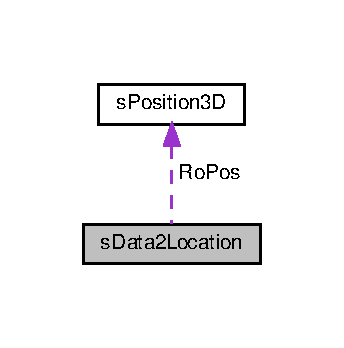
\includegraphics[width=165pt]{structs_data2_location__coll__graph}
\end{center}
\end{figure}
\subsection*{Public Attributes}
\begin{DoxyCompactItemize}
\item 
\hyperlink{_geometric_calc_8h_aabfa1dd0400b274a48b4a45afbee0af4}{Position3D} \hyperlink{structs_data2_location_abcac106c1692d71348a9184a194a9e02}{Ro\+Pos}
\item 
double \hyperlink{structs_data2_location_ae46f8fccbf91e76dc5c389bbf08ab927}{Heading\+Delta}
\item 
double \hyperlink{structs_data2_location_a989f56d96048891777a1ffdfec13fdab}{Rv\+Speed}
\item 
\hyperlink{_psd_location_8h_a6f150184d2a8f67d5c7de45bac365d15}{Event\+Classification} \hyperlink{structs_data2_location_ae207b6bc1ed4bb06e2b2f380f1ea6152}{event\+Classify}
\end{DoxyCompactItemize}


\subsection{Member Data Documentation}
\mbox{\Hypertarget{structs_data2_location_ae207b6bc1ed4bb06e2b2f380f1ea6152}\label{structs_data2_location_ae207b6bc1ed4bb06e2b2f380f1ea6152}} 
\index{s\+Data2\+Location@{s\+Data2\+Location}!event\+Classify@{event\+Classify}}
\index{event\+Classify@{event\+Classify}!s\+Data2\+Location@{s\+Data2\+Location}}
\subsubsection{\texorpdfstring{event\+Classify}{eventClassify}}
{\footnotesize\ttfamily \hyperlink{_psd_location_8h_a6f150184d2a8f67d5c7de45bac365d15}{Event\+Classification} s\+Data2\+Location\+::event\+Classify}

\mbox{\Hypertarget{structs_data2_location_ae46f8fccbf91e76dc5c389bbf08ab927}\label{structs_data2_location_ae46f8fccbf91e76dc5c389bbf08ab927}} 
\index{s\+Data2\+Location@{s\+Data2\+Location}!Heading\+Delta@{Heading\+Delta}}
\index{Heading\+Delta@{Heading\+Delta}!s\+Data2\+Location@{s\+Data2\+Location}}
\subsubsection{\texorpdfstring{Heading\+Delta}{HeadingDelta}}
{\footnotesize\ttfamily double s\+Data2\+Location\+::\+Heading\+Delta}

\mbox{\Hypertarget{structs_data2_location_abcac106c1692d71348a9184a194a9e02}\label{structs_data2_location_abcac106c1692d71348a9184a194a9e02}} 
\index{s\+Data2\+Location@{s\+Data2\+Location}!Ro\+Pos@{Ro\+Pos}}
\index{Ro\+Pos@{Ro\+Pos}!s\+Data2\+Location@{s\+Data2\+Location}}
\subsubsection{\texorpdfstring{Ro\+Pos}{RoPos}}
{\footnotesize\ttfamily \hyperlink{_geometric_calc_8h_aabfa1dd0400b274a48b4a45afbee0af4}{Position3D} s\+Data2\+Location\+::\+Ro\+Pos}

\mbox{\Hypertarget{structs_data2_location_a989f56d96048891777a1ffdfec13fdab}\label{structs_data2_location_a989f56d96048891777a1ffdfec13fdab}} 
\index{s\+Data2\+Location@{s\+Data2\+Location}!Rv\+Speed@{Rv\+Speed}}
\index{Rv\+Speed@{Rv\+Speed}!s\+Data2\+Location@{s\+Data2\+Location}}
\subsubsection{\texorpdfstring{Rv\+Speed}{RvSpeed}}
{\footnotesize\ttfamily double s\+Data2\+Location\+::\+Rv\+Speed}



The documentation for this struct was generated from the following file\+:\begin{DoxyCompactItemize}
\item 
src/\hyperlink{_psd_location_8h}{Psd\+Location.\+h}\end{DoxyCompactItemize}

\hypertarget{struct_self_segment}{}\section{Self\+Segment Struct Reference}
\label{struct_self_segment}\index{Self\+Segment@{Self\+Segment}}


{\ttfamily \#include $<$Psd\+Message\+Decoder.\+h$>$}



Collaboration diagram for Self\+Segment\+:\nopagebreak
\begin{figure}[H]
\begin{center}
\leavevmode
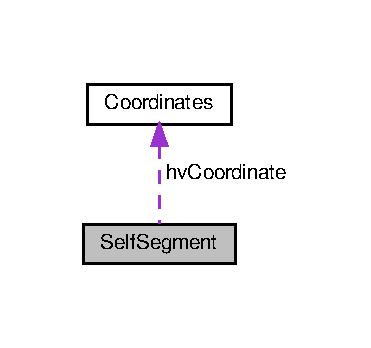
\includegraphics[width=178pt]{struct_self_segment__coll__graph}
\end{center}
\end{figure}
\subsection*{Public Attributes}
\begin{DoxyCompactItemize}
\item 
uint8\+\_\+t \hyperlink{struct_self_segment_a0bb36b5efe9c32319d685f13e458a5d0}{cur\+Segment\+Id}
\item 
uint8\+\_\+t \hyperlink{struct_self_segment_a2eb5169bc62a6c1945218e6a23a01aea}{cur\+Remain\+Length}
\item 
bool \hyperlink{struct_self_segment_adc13c811ad05f192237b55be4c2468bd}{pos\+Is\+Unique}
\item 
\hyperlink{_psd_message_decoder_8h_a954d216bca8cdfc325504c05bb6c4336}{e\+\_\+\+Pos\+Length\+Err} \hyperlink{struct_self_segment_a3fb749f98032e0f439c64722cdcc7cea}{pos\+Length\+Err}
\item 
uint8\+\_\+t \hyperlink{struct_self_segment_a288eff27cbe3c5986dbdacfd12141675}{last\+Segment\+Id}
\item 
\hyperlink{_psd_message_decoder_8h_a559ada7297c8c6c2337f9e233e73aeca}{t\+Coordinates} \hyperlink{struct_self_segment_a7777e101b62ea11f2030bbe078cb4557}{hv\+Coordinate}
\item 
double \hyperlink{struct_self_segment_a05eb5f224252e2c1e7d29b7da69b2dc2}{hv\+Heading}
\end{DoxyCompactItemize}


\subsection{Member Data Documentation}
\mbox{\Hypertarget{struct_self_segment_a2eb5169bc62a6c1945218e6a23a01aea}\label{struct_self_segment_a2eb5169bc62a6c1945218e6a23a01aea}} 
\index{Self\+Segment@{Self\+Segment}!cur\+Remain\+Length@{cur\+Remain\+Length}}
\index{cur\+Remain\+Length@{cur\+Remain\+Length}!Self\+Segment@{Self\+Segment}}
\subsubsection{\texorpdfstring{cur\+Remain\+Length}{curRemainLength}}
{\footnotesize\ttfamily uint8\+\_\+t Self\+Segment\+::cur\+Remain\+Length}

\mbox{\Hypertarget{struct_self_segment_a0bb36b5efe9c32319d685f13e458a5d0}\label{struct_self_segment_a0bb36b5efe9c32319d685f13e458a5d0}} 
\index{Self\+Segment@{Self\+Segment}!cur\+Segment\+Id@{cur\+Segment\+Id}}
\index{cur\+Segment\+Id@{cur\+Segment\+Id}!Self\+Segment@{Self\+Segment}}
\subsubsection{\texorpdfstring{cur\+Segment\+Id}{curSegmentId}}
{\footnotesize\ttfamily uint8\+\_\+t Self\+Segment\+::cur\+Segment\+Id}

\mbox{\Hypertarget{struct_self_segment_a7777e101b62ea11f2030bbe078cb4557}\label{struct_self_segment_a7777e101b62ea11f2030bbe078cb4557}} 
\index{Self\+Segment@{Self\+Segment}!hv\+Coordinate@{hv\+Coordinate}}
\index{hv\+Coordinate@{hv\+Coordinate}!Self\+Segment@{Self\+Segment}}
\subsubsection{\texorpdfstring{hv\+Coordinate}{hvCoordinate}}
{\footnotesize\ttfamily \hyperlink{_psd_message_decoder_8h_a559ada7297c8c6c2337f9e233e73aeca}{t\+Coordinates} Self\+Segment\+::hv\+Coordinate}

\mbox{\Hypertarget{struct_self_segment_a05eb5f224252e2c1e7d29b7da69b2dc2}\label{struct_self_segment_a05eb5f224252e2c1e7d29b7da69b2dc2}} 
\index{Self\+Segment@{Self\+Segment}!hv\+Heading@{hv\+Heading}}
\index{hv\+Heading@{hv\+Heading}!Self\+Segment@{Self\+Segment}}
\subsubsection{\texorpdfstring{hv\+Heading}{hvHeading}}
{\footnotesize\ttfamily double Self\+Segment\+::hv\+Heading}

\mbox{\Hypertarget{struct_self_segment_a288eff27cbe3c5986dbdacfd12141675}\label{struct_self_segment_a288eff27cbe3c5986dbdacfd12141675}} 
\index{Self\+Segment@{Self\+Segment}!last\+Segment\+Id@{last\+Segment\+Id}}
\index{last\+Segment\+Id@{last\+Segment\+Id}!Self\+Segment@{Self\+Segment}}
\subsubsection{\texorpdfstring{last\+Segment\+Id}{lastSegmentId}}
{\footnotesize\ttfamily uint8\+\_\+t Self\+Segment\+::last\+Segment\+Id}

\mbox{\Hypertarget{struct_self_segment_adc13c811ad05f192237b55be4c2468bd}\label{struct_self_segment_adc13c811ad05f192237b55be4c2468bd}} 
\index{Self\+Segment@{Self\+Segment}!pos\+Is\+Unique@{pos\+Is\+Unique}}
\index{pos\+Is\+Unique@{pos\+Is\+Unique}!Self\+Segment@{Self\+Segment}}
\subsubsection{\texorpdfstring{pos\+Is\+Unique}{posIsUnique}}
{\footnotesize\ttfamily bool Self\+Segment\+::pos\+Is\+Unique}

\mbox{\Hypertarget{struct_self_segment_a3fb749f98032e0f439c64722cdcc7cea}\label{struct_self_segment_a3fb749f98032e0f439c64722cdcc7cea}} 
\index{Self\+Segment@{Self\+Segment}!pos\+Length\+Err@{pos\+Length\+Err}}
\index{pos\+Length\+Err@{pos\+Length\+Err}!Self\+Segment@{Self\+Segment}}
\subsubsection{\texorpdfstring{pos\+Length\+Err}{posLengthErr}}
{\footnotesize\ttfamily \hyperlink{_psd_message_decoder_8h_a954d216bca8cdfc325504c05bb6c4336}{e\+\_\+\+Pos\+Length\+Err} Self\+Segment\+::pos\+Length\+Err}



The documentation for this struct was generated from the following file\+:\begin{DoxyCompactItemize}
\item 
src/\hyperlink{_psd_message_decoder_8h}{Psd\+Message\+Decoder.\+h}\end{DoxyCompactItemize}

\hypertarget{structs_position3_d}{}\section{s\+Position3D Struct Reference}
\label{structs_position3_d}\index{s\+Position3D@{s\+Position3D}}


{\ttfamily \#include $<$Geometric\+Calc.\+h$>$}

\subsection*{Public Attributes}
\begin{DoxyCompactItemize}
\item 
double \hyperlink{structs_position3_d_a0e4b0c9062c6078595bc52f7f44b6ab5}{lat}
\item 
double \hyperlink{structs_position3_d_a20077e90edce2375772932e068c47118}{lon}
\item 
double \hyperlink{structs_position3_d_a5cc5aa32a6588b19d7666007525c6e9d}{elevation}
\end{DoxyCompactItemize}


\subsection{Member Data Documentation}
\mbox{\Hypertarget{structs_position3_d_a5cc5aa32a6588b19d7666007525c6e9d}\label{structs_position3_d_a5cc5aa32a6588b19d7666007525c6e9d}} 
\index{s\+Position3D@{s\+Position3D}!elevation@{elevation}}
\index{elevation@{elevation}!s\+Position3D@{s\+Position3D}}
\subsubsection{\texorpdfstring{elevation}{elevation}}
{\footnotesize\ttfamily double s\+Position3\+D\+::elevation}

\mbox{\Hypertarget{structs_position3_d_a0e4b0c9062c6078595bc52f7f44b6ab5}\label{structs_position3_d_a0e4b0c9062c6078595bc52f7f44b6ab5}} 
\index{s\+Position3D@{s\+Position3D}!lat@{lat}}
\index{lat@{lat}!s\+Position3D@{s\+Position3D}}
\subsubsection{\texorpdfstring{lat}{lat}}
{\footnotesize\ttfamily double s\+Position3\+D\+::lat}

\mbox{\Hypertarget{structs_position3_d_a20077e90edce2375772932e068c47118}\label{structs_position3_d_a20077e90edce2375772932e068c47118}} 
\index{s\+Position3D@{s\+Position3D}!lon@{lon}}
\index{lon@{lon}!s\+Position3D@{s\+Position3D}}
\subsubsection{\texorpdfstring{lon}{lon}}
{\footnotesize\ttfamily double s\+Position3\+D\+::lon}



The documentation for this struct was generated from the following file\+:\begin{DoxyCompactItemize}
\item 
src/\hyperlink{_geometric_calc_8h}{Geometric\+Calc.\+h}\end{DoxyCompactItemize}

\hypertarget{structt_point}{}\section{t\+Point Struct Reference}
\label{structt_point}\index{t\+Point@{t\+Point}}


{\ttfamily \#include $<$Geometric\+Calc.\+h$>$}

\subsection*{Public Attributes}
\begin{DoxyCompactItemize}
\item 
double \hyperlink{structt_point_a00e0256537c88142b0618b1286504b73}{x}
\item 
double \hyperlink{structt_point_af251026a3efb5fe7f96ff65af3b93e50}{y}
\end{DoxyCompactItemize}


\subsection{Member Data Documentation}
\mbox{\Hypertarget{structt_point_a00e0256537c88142b0618b1286504b73}\label{structt_point_a00e0256537c88142b0618b1286504b73}} 
\index{t\+Point@{t\+Point}!x@{x}}
\index{x@{x}!t\+Point@{t\+Point}}
\subsubsection{\texorpdfstring{x}{x}}
{\footnotesize\ttfamily double t\+Point\+::x}

\mbox{\Hypertarget{structt_point_af251026a3efb5fe7f96ff65af3b93e50}\label{structt_point_af251026a3efb5fe7f96ff65af3b93e50}} 
\index{t\+Point@{t\+Point}!y@{y}}
\index{y@{y}!t\+Point@{t\+Point}}
\subsubsection{\texorpdfstring{y}{y}}
{\footnotesize\ttfamily double t\+Point\+::y}



The documentation for this struct was generated from the following file\+:\begin{DoxyCompactItemize}
\item 
src/\hyperlink{_geometric_calc_8h}{Geometric\+Calc.\+h}\end{DoxyCompactItemize}

\hypertarget{struct_tree_node}{}\section{Tree\+Node Struct Reference}
\label{struct_tree_node}\index{Tree\+Node@{Tree\+Node}}


{\ttfamily \#include $<$Psd\+Map.\+h$>$}



Collaboration diagram for Tree\+Node\+:\nopagebreak
\begin{figure}[H]
\begin{center}
\leavevmode
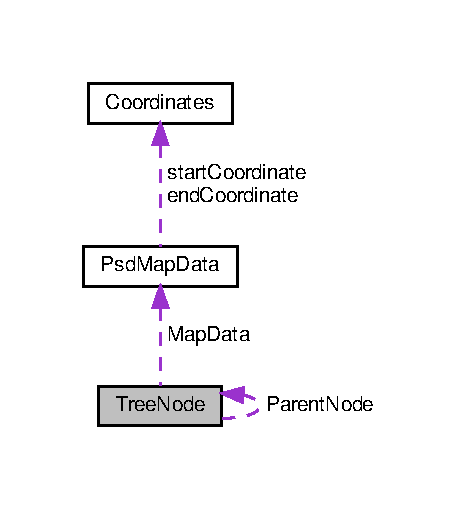
\includegraphics[width=220pt]{struct_tree_node__coll__graph}
\end{center}
\end{figure}
\subsection*{Public Attributes}
\begin{DoxyCompactItemize}
\item 
\hyperlink{_psd_message_decoder_8h_ad54e183dd7c544312c06d4bd6279ebdc}{t\+Psd\+Map\+Data} \hyperlink{struct_tree_node_a37bb860a60a8145caa4d2d2227f72e8b}{Map\+Data}
\item 
struct \hyperlink{struct_tree_node}{Tree\+Node} $\ast$ \hyperlink{struct_tree_node_a2e4d7b1482b67b0be9a09ba86e225300}{Parent\+Node}
\item 
std\+::vector$<$ struct \hyperlink{struct_tree_node}{Tree\+Node} $\ast$ $>$ \hyperlink{struct_tree_node_adb4d9e37e7a3b5fddbabf56ac56eccd7}{v\+Childs}
\end{DoxyCompactItemize}


\subsection{Member Data Documentation}
\mbox{\Hypertarget{struct_tree_node_a37bb860a60a8145caa4d2d2227f72e8b}\label{struct_tree_node_a37bb860a60a8145caa4d2d2227f72e8b}} 
\index{Tree\+Node@{Tree\+Node}!Map\+Data@{Map\+Data}}
\index{Map\+Data@{Map\+Data}!Tree\+Node@{Tree\+Node}}
\subsubsection{\texorpdfstring{Map\+Data}{MapData}}
{\footnotesize\ttfamily \hyperlink{_psd_message_decoder_8h_ad54e183dd7c544312c06d4bd6279ebdc}{t\+Psd\+Map\+Data} Tree\+Node\+::\+Map\+Data}

\mbox{\Hypertarget{struct_tree_node_a2e4d7b1482b67b0be9a09ba86e225300}\label{struct_tree_node_a2e4d7b1482b67b0be9a09ba86e225300}} 
\index{Tree\+Node@{Tree\+Node}!Parent\+Node@{Parent\+Node}}
\index{Parent\+Node@{Parent\+Node}!Tree\+Node@{Tree\+Node}}
\subsubsection{\texorpdfstring{Parent\+Node}{ParentNode}}
{\footnotesize\ttfamily struct \hyperlink{struct_tree_node}{Tree\+Node}$\ast$ Tree\+Node\+::\+Parent\+Node}

\mbox{\Hypertarget{struct_tree_node_adb4d9e37e7a3b5fddbabf56ac56eccd7}\label{struct_tree_node_adb4d9e37e7a3b5fddbabf56ac56eccd7}} 
\index{Tree\+Node@{Tree\+Node}!v\+Childs@{v\+Childs}}
\index{v\+Childs@{v\+Childs}!Tree\+Node@{Tree\+Node}}
\subsubsection{\texorpdfstring{v\+Childs}{vChilds}}
{\footnotesize\ttfamily std\+::vector$<$ struct \hyperlink{struct_tree_node}{Tree\+Node} $\ast$$>$ Tree\+Node\+::v\+Childs}



The documentation for this struct was generated from the following file\+:\begin{DoxyCompactItemize}
\item 
src/\hyperlink{_psd_map_8h}{Psd\+Map.\+h}\end{DoxyCompactItemize}

\chapter{File Documentation}
\hypertarget{_geometric_calc_8cpp}{}\section{src/\+Geometric\+Calc.cpp File Reference}
\label{_geometric_calc_8cpp}\index{src/\+Geometric\+Calc.\+cpp@{src/\+Geometric\+Calc.\+cpp}}
{\ttfamily \#include \char`\"{}../inc/\+Geometric\+Calc.\+h\char`\"{}}\newline
{\ttfamily \#include $<$cstdio$>$}\newline
{\ttfamily \#include $<$cmath$>$}\newline
Include dependency graph for Geometric\+Calc.\+cpp\+:
\nopagebreak
\begin{figure}[H]
\begin{center}
\leavevmode
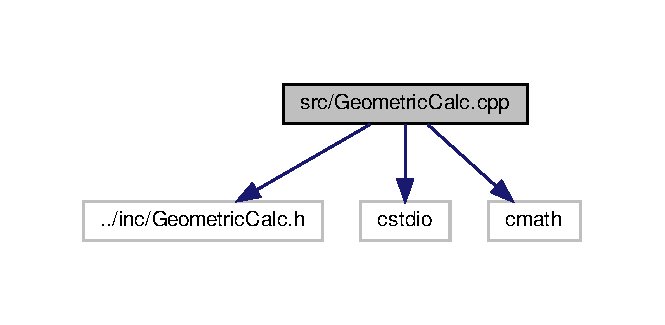
\includegraphics[width=319pt]{_geometric_calc_8cpp__incl}
\end{center}
\end{figure}

\hypertarget{_geometric_calc_8h}{}\section{src/\+Geometric\+Calc.h File Reference}
\label{_geometric_calc_8h}\index{src/\+Geometric\+Calc.\+h@{src/\+Geometric\+Calc.\+h}}
This graph shows which files directly or indirectly include this file\+:
\nopagebreak
\begin{figure}[H]
\begin{center}
\leavevmode
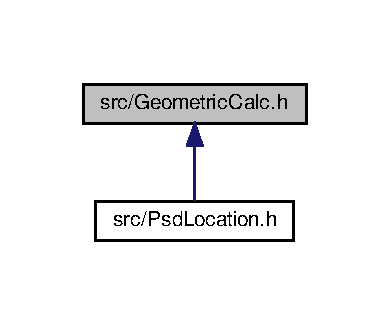
\includegraphics[width=187pt]{_geometric_calc_8h__dep__incl}
\end{center}
\end{figure}
\subsection*{Classes}
\begin{DoxyCompactItemize}
\item 
struct \hyperlink{structs_position3_d}{s\+Position3D}
\item 
struct \hyperlink{structt_point}{t\+Point}
\item 
class \hyperlink{class_geometric_calc}{Geometric\+Calc}
\end{DoxyCompactItemize}
\subsection*{Typedefs}
\begin{DoxyCompactItemize}
\item 
typedef struct \hyperlink{structs_position3_d}{s\+Position3D} \hyperlink{_geometric_calc_8h_aabfa1dd0400b274a48b4a45afbee0af4}{Position3D}
\item 
typedef struct \hyperlink{structt_point}{t\+Point} \hyperlink{_geometric_calc_8h_a7d6013bdb30e1e3c07a3d84518d395dc}{Point}
\end{DoxyCompactItemize}


\subsection{Typedef Documentation}
\mbox{\Hypertarget{_geometric_calc_8h_a7d6013bdb30e1e3c07a3d84518d395dc}\label{_geometric_calc_8h_a7d6013bdb30e1e3c07a3d84518d395dc}} 
\index{Geometric\+Calc.\+h@{Geometric\+Calc.\+h}!Point@{Point}}
\index{Point@{Point}!Geometric\+Calc.\+h@{Geometric\+Calc.\+h}}
\subsubsection{\texorpdfstring{Point}{Point}}
{\footnotesize\ttfamily typedef struct \hyperlink{structt_point}{t\+Point} \hyperlink{_geometric_calc_8h_a7d6013bdb30e1e3c07a3d84518d395dc}{Point}}

\mbox{\Hypertarget{_geometric_calc_8h_aabfa1dd0400b274a48b4a45afbee0af4}\label{_geometric_calc_8h_aabfa1dd0400b274a48b4a45afbee0af4}} 
\index{Geometric\+Calc.\+h@{Geometric\+Calc.\+h}!Position3D@{Position3D}}
\index{Position3D@{Position3D}!Geometric\+Calc.\+h@{Geometric\+Calc.\+h}}
\subsubsection{\texorpdfstring{Position3D}{Position3D}}
{\footnotesize\ttfamily typedef struct \hyperlink{structs_position3_d}{s\+Position3D} \hyperlink{_geometric_calc_8h_aabfa1dd0400b274a48b4a45afbee0af4}{Position3D}}


\hypertarget{_haversine_8cpp}{}\section{src/\+Haversine.cpp File Reference}
\label{_haversine_8cpp}\index{src/\+Haversine.\+cpp@{src/\+Haversine.\+cpp}}
{\ttfamily \#include \char`\"{}../inc/\+Haversine.\+h\char`\"{}}\newline
{\ttfamily \#include $<$cstdio$>$}\newline
{\ttfamily \#include $<$cmath$>$}\newline
Include dependency graph for Haversine.\+cpp\+:\nopagebreak
\begin{figure}[H]
\begin{center}
\leavevmode
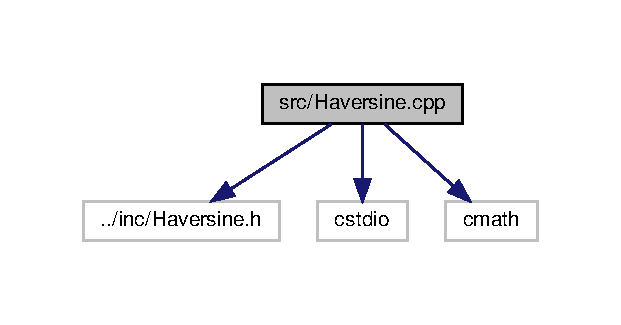
\includegraphics[width=298pt]{_haversine_8cpp__incl}
\end{center}
\end{figure}
\subsection*{Macros}
\begin{DoxyCompactItemize}
\item 
\#define \hyperlink{_haversine_8cpp_a598a3330b3c21701223ee0ca14316eca}{PI}~acos(-\/1)
\item 
\#define \hyperlink{_haversine_8cpp_aacdf1719d113d68a71127426f7c730cd}{E\+A\+R\+T\+H\+\_\+\+R\+A\+D\+I\+US}~6378.\+137
\end{DoxyCompactItemize}


\subsection{Macro Definition Documentation}
\mbox{\Hypertarget{_haversine_8cpp_aacdf1719d113d68a71127426f7c730cd}\label{_haversine_8cpp_aacdf1719d113d68a71127426f7c730cd}} 
\index{Haversine.\+cpp@{Haversine.\+cpp}!E\+A\+R\+T\+H\+\_\+\+R\+A\+D\+I\+US@{E\+A\+R\+T\+H\+\_\+\+R\+A\+D\+I\+US}}
\index{E\+A\+R\+T\+H\+\_\+\+R\+A\+D\+I\+US@{E\+A\+R\+T\+H\+\_\+\+R\+A\+D\+I\+US}!Haversine.\+cpp@{Haversine.\+cpp}}
\subsubsection{\texorpdfstring{E\+A\+R\+T\+H\+\_\+\+R\+A\+D\+I\+US}{EARTH\_RADIUS}}
{\footnotesize\ttfamily \#define E\+A\+R\+T\+H\+\_\+\+R\+A\+D\+I\+US~6378.\+137}

\mbox{\Hypertarget{_haversine_8cpp_a598a3330b3c21701223ee0ca14316eca}\label{_haversine_8cpp_a598a3330b3c21701223ee0ca14316eca}} 
\index{Haversine.\+cpp@{Haversine.\+cpp}!PI@{PI}}
\index{PI@{PI}!Haversine.\+cpp@{Haversine.\+cpp}}
\subsubsection{\texorpdfstring{PI}{PI}}
{\footnotesize\ttfamily \#define PI~acos(-\/1)}


\hypertarget{_haversine_8h}{}\section{src/\+Haversine.h File Reference}
\label{_haversine_8h}\index{src/\+Haversine.\+h@{src/\+Haversine.\+h}}
{\ttfamily \#include \char`\"{}Psd\+Message\+Decoder.\+h\char`\"{}}\newline
Include dependency graph for Haversine.\+h\+:\nopagebreak
\begin{figure}[H]
\begin{center}
\leavevmode
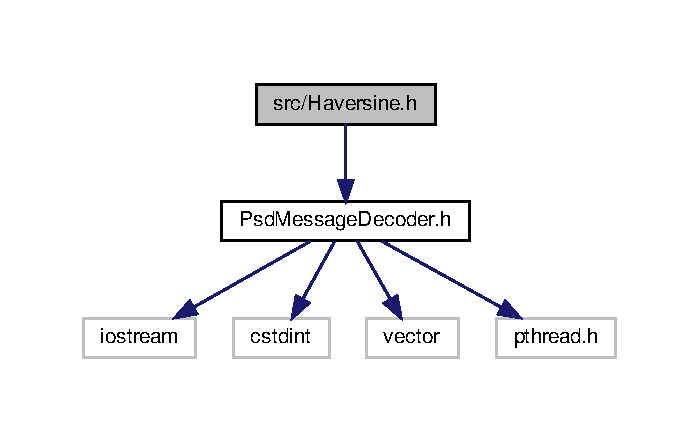
\includegraphics[width=336pt]{_haversine_8h__incl}
\end{center}
\end{figure}
This graph shows which files directly or indirectly include this file\+:
\nopagebreak
\begin{figure}[H]
\begin{center}
\leavevmode
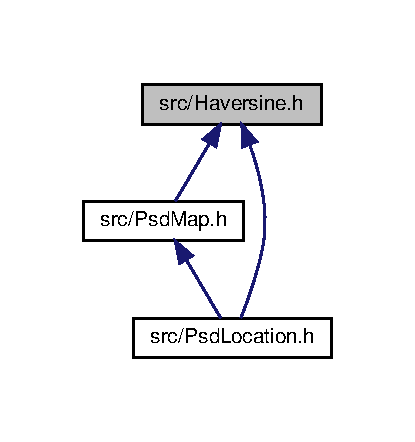
\includegraphics[width=199pt]{_haversine_8h__dep__incl}
\end{center}
\end{figure}
\subsection*{Classes}
\begin{DoxyCompactItemize}
\item 
struct \hyperlink{struct_angle}{Angle}
\item 
class \hyperlink{class_haversine}{Haversine}
\end{DoxyCompactItemize}
\subsection*{Typedefs}
\begin{DoxyCompactItemize}
\item 
typedef struct \hyperlink{struct_angle}{Angle} \hyperlink{_haversine_8h_a6ff61bf38ccfdf0cc520e0fed7406b4b}{t\+Angle}
\end{DoxyCompactItemize}


\subsection{Typedef Documentation}
\mbox{\Hypertarget{_haversine_8h_a6ff61bf38ccfdf0cc520e0fed7406b4b}\label{_haversine_8h_a6ff61bf38ccfdf0cc520e0fed7406b4b}} 
\index{Haversine.\+h@{Haversine.\+h}!t\+Angle@{t\+Angle}}
\index{t\+Angle@{t\+Angle}!Haversine.\+h@{Haversine.\+h}}
\subsubsection{\texorpdfstring{t\+Angle}{tAngle}}
{\footnotesize\ttfamily typedef struct \hyperlink{struct_angle}{Angle} \hyperlink{_haversine_8h_a6ff61bf38ccfdf0cc520e0fed7406b4b}{t\+Angle}}


\hypertarget{_psd_location_8cpp}{}\section{src/\+Psd\+Location.cpp File Reference}
\label{_psd_location_8cpp}\index{src/\+Psd\+Location.\+cpp@{src/\+Psd\+Location.\+cpp}}
{\ttfamily \#include $<$cstdio$>$}\newline
{\ttfamily \#include $<$algorithm$>$}\newline
{\ttfamily \#include $<$cmath$>$}\newline
{\ttfamily \#include $<$cstring$>$}\newline
{\ttfamily \#include \char`\"{}../inc/\+Psd\+Location.\+h\char`\"{}}\newline
{\ttfamily \#include \char`\"{}../inc/\+Geometric\+Calc.\+h\char`\"{}}\newline
Include dependency graph for Psd\+Location.\+cpp\+:
\nopagebreak
\begin{figure}[H]
\begin{center}
\leavevmode
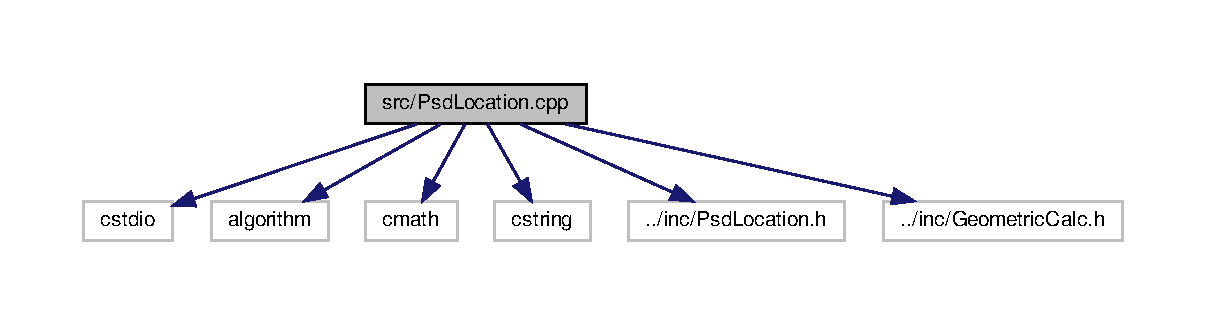
\includegraphics[width=350pt]{_psd_location_8cpp__incl}
\end{center}
\end{figure}
\subsection*{Functions}
\begin{DoxyCompactItemize}
\item 
void $\ast$ \hyperlink{_psd_location_8cpp_ab233e13620a7fae2a5576ccf9d70f590}{Psd\+Map\+Run} (void $\ast$arg)
\item 
void $\ast$ \hyperlink{_psd_location_8cpp_a99afa19c7e74376d95279fd72d4febef}{Psd\+Message\+Decoder\+Run} (void $\ast$arg)
\end{DoxyCompactItemize}
\subsection*{Variables}
\begin{DoxyCompactItemize}
\item 
pthread\+\_\+mutex\+\_\+t \hyperlink{_psd_location_8cpp_a0e54b67a9bf300f936f9e747986659a4}{decoder\+Thread\+Mutex}
\item 
pthread\+\_\+mutex\+\_\+t \hyperlink{_psd_location_8cpp_aabb1d569e89cf787398ffc1a0a3b536c}{map\+Thread\+Mutex}
\item 
bool \hyperlink{_psd_location_8cpp_ae48c69ffd0bb85b3a053532b8bd93a9f}{p\+Psd\+Usage\+Active} = 0
\item 
double \hyperlink{_psd_location_8cpp_a2ed204372662d6323173bea09cf77019}{p\+Lateral\+Dist\+Tolerance} = 8.\+0
\item 
double \hyperlink{_psd_location_8cpp_aff6445ba91fa259a3b39fb722c1be639}{p\+Relative\+Position\+Angle} = 45.\+0
\item 
double \hyperlink{_psd_location_8cpp_ad0836fca0c35617f4eee507efe90b970}{p\+Relative\+Direction} = 45.\+0
\item 
double \hyperlink{_psd_location_8cpp_a37f4203003143e655056c0825b855a7b}{p\+Stationary\+Threshold} = 50.\+0
\end{DoxyCompactItemize}


\subsection{Function Documentation}
\mbox{\Hypertarget{_psd_location_8cpp_ab233e13620a7fae2a5576ccf9d70f590}\label{_psd_location_8cpp_ab233e13620a7fae2a5576ccf9d70f590}} 
\index{Psd\+Location.\+cpp@{Psd\+Location.\+cpp}!Psd\+Map\+Run@{Psd\+Map\+Run}}
\index{Psd\+Map\+Run@{Psd\+Map\+Run}!Psd\+Location.\+cpp@{Psd\+Location.\+cpp}}
\subsubsection{\texorpdfstring{Psd\+Map\+Run()}{PsdMapRun()}}
{\footnotesize\ttfamily void$\ast$ Psd\+Map\+Run (\begin{DoxyParamCaption}\item[{void $\ast$}]{arg }\end{DoxyParamCaption})}

\mbox{\Hypertarget{_psd_location_8cpp_a99afa19c7e74376d95279fd72d4febef}\label{_psd_location_8cpp_a99afa19c7e74376d95279fd72d4febef}} 
\index{Psd\+Location.\+cpp@{Psd\+Location.\+cpp}!Psd\+Message\+Decoder\+Run@{Psd\+Message\+Decoder\+Run}}
\index{Psd\+Message\+Decoder\+Run@{Psd\+Message\+Decoder\+Run}!Psd\+Location.\+cpp@{Psd\+Location.\+cpp}}
\subsubsection{\texorpdfstring{Psd\+Message\+Decoder\+Run()}{PsdMessageDecoderRun()}}
{\footnotesize\ttfamily void$\ast$ Psd\+Message\+Decoder\+Run (\begin{DoxyParamCaption}\item[{void $\ast$}]{arg }\end{DoxyParamCaption})}



\subsection{Variable Documentation}
\mbox{\Hypertarget{_psd_location_8cpp_a0e54b67a9bf300f936f9e747986659a4}\label{_psd_location_8cpp_a0e54b67a9bf300f936f9e747986659a4}} 
\index{Psd\+Location.\+cpp@{Psd\+Location.\+cpp}!decoder\+Thread\+Mutex@{decoder\+Thread\+Mutex}}
\index{decoder\+Thread\+Mutex@{decoder\+Thread\+Mutex}!Psd\+Location.\+cpp@{Psd\+Location.\+cpp}}
\subsubsection{\texorpdfstring{decoder\+Thread\+Mutex}{decoderThreadMutex}}
{\footnotesize\ttfamily pthread\+\_\+mutex\+\_\+t decoder\+Thread\+Mutex}

\mbox{\Hypertarget{_psd_location_8cpp_aabb1d569e89cf787398ffc1a0a3b536c}\label{_psd_location_8cpp_aabb1d569e89cf787398ffc1a0a3b536c}} 
\index{Psd\+Location.\+cpp@{Psd\+Location.\+cpp}!map\+Thread\+Mutex@{map\+Thread\+Mutex}}
\index{map\+Thread\+Mutex@{map\+Thread\+Mutex}!Psd\+Location.\+cpp@{Psd\+Location.\+cpp}}
\subsubsection{\texorpdfstring{map\+Thread\+Mutex}{mapThreadMutex}}
{\footnotesize\ttfamily pthread\+\_\+mutex\+\_\+t map\+Thread\+Mutex}

\mbox{\Hypertarget{_psd_location_8cpp_a2ed204372662d6323173bea09cf77019}\label{_psd_location_8cpp_a2ed204372662d6323173bea09cf77019}} 
\index{Psd\+Location.\+cpp@{Psd\+Location.\+cpp}!p\+Lateral\+Dist\+Tolerance@{p\+Lateral\+Dist\+Tolerance}}
\index{p\+Lateral\+Dist\+Tolerance@{p\+Lateral\+Dist\+Tolerance}!Psd\+Location.\+cpp@{Psd\+Location.\+cpp}}
\subsubsection{\texorpdfstring{p\+Lateral\+Dist\+Tolerance}{pLateralDistTolerance}}
{\footnotesize\ttfamily double p\+Lateral\+Dist\+Tolerance = 8.\+0}

$<$ p\+\_\+\+P\+S\+D\+\_\+\+Usage\+\_\+\+Active \mbox{\Hypertarget{_psd_location_8cpp_ae48c69ffd0bb85b3a053532b8bd93a9f}\label{_psd_location_8cpp_ae48c69ffd0bb85b3a053532b8bd93a9f}} 
\index{Psd\+Location.\+cpp@{Psd\+Location.\+cpp}!p\+Psd\+Usage\+Active@{p\+Psd\+Usage\+Active}}
\index{p\+Psd\+Usage\+Active@{p\+Psd\+Usage\+Active}!Psd\+Location.\+cpp@{Psd\+Location.\+cpp}}
\subsubsection{\texorpdfstring{p\+Psd\+Usage\+Active}{pPsdUsageActive}}
{\footnotesize\ttfamily bool p\+Psd\+Usage\+Active = 0}

\mbox{\Hypertarget{_psd_location_8cpp_ad0836fca0c35617f4eee507efe90b970}\label{_psd_location_8cpp_ad0836fca0c35617f4eee507efe90b970}} 
\index{Psd\+Location.\+cpp@{Psd\+Location.\+cpp}!p\+Relative\+Direction@{p\+Relative\+Direction}}
\index{p\+Relative\+Direction@{p\+Relative\+Direction}!Psd\+Location.\+cpp@{Psd\+Location.\+cpp}}
\subsubsection{\texorpdfstring{p\+Relative\+Direction}{pRelativeDirection}}
{\footnotesize\ttfamily double p\+Relative\+Direction = 45.\+0}

$<$ p\+\_\+relative\+\_\+position\+\_\+angle, default value == 45 degrees \mbox{\Hypertarget{_psd_location_8cpp_aff6445ba91fa259a3b39fb722c1be639}\label{_psd_location_8cpp_aff6445ba91fa259a3b39fb722c1be639}} 
\index{Psd\+Location.\+cpp@{Psd\+Location.\+cpp}!p\+Relative\+Position\+Angle@{p\+Relative\+Position\+Angle}}
\index{p\+Relative\+Position\+Angle@{p\+Relative\+Position\+Angle}!Psd\+Location.\+cpp@{Psd\+Location.\+cpp}}
\subsubsection{\texorpdfstring{p\+Relative\+Position\+Angle}{pRelativePositionAngle}}
{\footnotesize\ttfamily double p\+Relative\+Position\+Angle = 45.\+0}

$<$ p\+\_\+lateral\+\_\+dist\+\_\+tolerance \mbox{\Hypertarget{_psd_location_8cpp_a37f4203003143e655056c0825b855a7b}\label{_psd_location_8cpp_a37f4203003143e655056c0825b855a7b}} 
\index{Psd\+Location.\+cpp@{Psd\+Location.\+cpp}!p\+Stationary\+Threshold@{p\+Stationary\+Threshold}}
\index{p\+Stationary\+Threshold@{p\+Stationary\+Threshold}!Psd\+Location.\+cpp@{Psd\+Location.\+cpp}}
\subsubsection{\texorpdfstring{p\+Stationary\+Threshold}{pStationaryThreshold}}
{\footnotesize\ttfamily double p\+Stationary\+Threshold = 50.\+0}

$<$ p\+\_\+relative\+\_\+direction, default value == 45 degrees 
\hypertarget{_psd_location_8h}{}\section{src/\+Psd\+Location.h File Reference}
\label{_psd_location_8h}\index{src/\+Psd\+Location.\+h@{src/\+Psd\+Location.\+h}}
{\ttfamily \#include \char`\"{}Psd\+Message\+Decoder.\+h\char`\"{}}\newline
{\ttfamily \#include \char`\"{}Psd\+Map.\+h\char`\"{}}\newline
{\ttfamily \#include \char`\"{}Haversine.\+h\char`\"{}}\newline
{\ttfamily \#include \char`\"{}Geometric\+Calc.\+h\char`\"{}}\newline
Include dependency graph for Psd\+Location.\+h\+:
\nopagebreak
\begin{figure}[H]
\begin{center}
\leavevmode
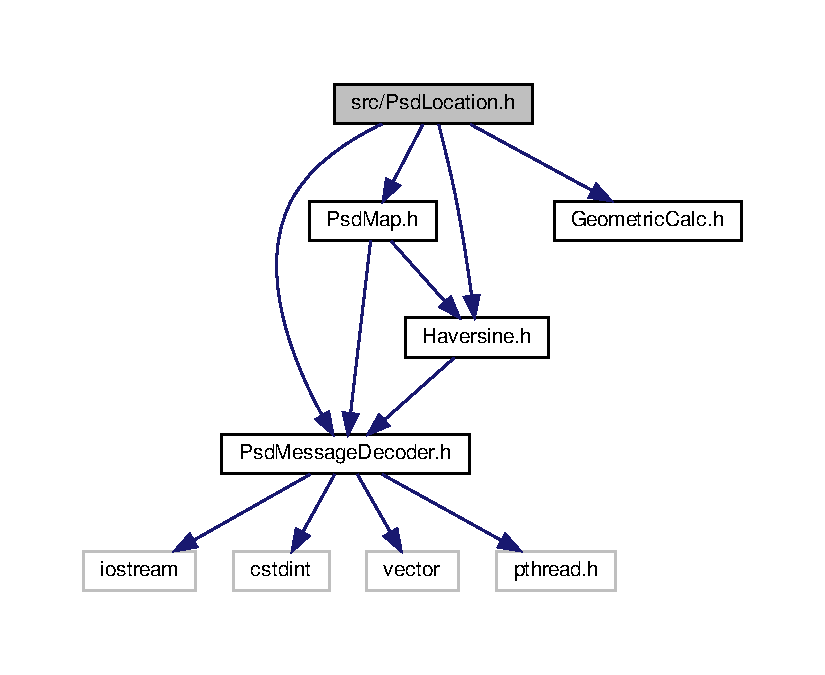
\includegraphics[width=350pt]{_psd_location_8h__incl}
\end{center}
\end{figure}
\subsection*{Classes}
\begin{DoxyCompactItemize}
\item 
struct \hyperlink{structs_data2_event_list}{s\+Data2\+Event\+List}
\item 
struct \hyperlink{structs_data2_location}{s\+Data2\+Location}
\item 
class \hyperlink{class_psd_location}{Psd\+Location}
\end{DoxyCompactItemize}
\subsection*{Typedefs}
\begin{DoxyCompactItemize}
\item 
typedef enum \hyperlink{_psd_location_8h_a515a8978c6db10bc2f63ce7c56539fca}{e\+Relevancy\+Check} \hyperlink{_psd_location_8h_ad3abb902810ad80bbc508a024f5af264}{Relevancy\+Check}
\item 
typedef enum \hyperlink{_psd_location_8h_ac41e0ae97d4220716d35997e4c83326a}{e\+Relative\+Position} \hyperlink{_psd_location_8h_abcb85fd51379afdf750bdda1dec9174c}{Relative\+Position}
\item 
typedef enum \hyperlink{_psd_location_8h_a6bd966d3120fc76f9fb619a81c961e09}{e\+Realative\+Direction} \hyperlink{_psd_location_8h_ae65d9d286580719610837075ffad7232}{Realative\+Direction}
\item 
typedef enum \hyperlink{_psd_location_8h_a5f47fe2a3f3518c41e21ae0004fcc09c}{e\+Event\+Classification} \hyperlink{_psd_location_8h_a6f150184d2a8f67d5c7de45bac365d15}{Event\+Classification}
\item 
typedef struct \hyperlink{structs_data2_event_list}{s\+Data2\+Event\+List} \hyperlink{_psd_location_8h_a61af0449f917913c902b37ed397eb350}{Data2\+Event\+List}
\item 
typedef struct \hyperlink{structs_data2_location}{s\+Data2\+Location} \hyperlink{_psd_location_8h_a1e3a92020005d2a81aa50ba5ae9b129c}{Data2\+Location}
\end{DoxyCompactItemize}
\subsection*{Enumerations}
\begin{DoxyCompactItemize}
\item 
enum \hyperlink{_psd_location_8h_a515a8978c6db10bc2f63ce7c56539fca}{e\+Relevancy\+Check} \{ \hyperlink{_psd_location_8h_a515a8978c6db10bc2f63ce7c56539fcaacb0ad5dc594fe5cb581ff0a792390f55}{irrelevant} = 0, 
\hyperlink{_psd_location_8h_a515a8978c6db10bc2f63ce7c56539fcaa9f59d9082ba0fc5eac32e3bef10fdf1b}{relevant} = 1
 \}
\item 
enum \hyperlink{_psd_location_8h_ac41e0ae97d4220716d35997e4c83326a}{e\+Relative\+Position} \{ \newline
\hyperlink{_psd_location_8h_ac41e0ae97d4220716d35997e4c83326aadc8544ceb1665156bc9c75e1508587ae}{Pos\+\_\+\+Unclassified} = 0, 
\hyperlink{_psd_location_8h_ac41e0ae97d4220716d35997e4c83326aa5ce6ffcda1927d36083af2417589aab9}{Pos\+\_\+\+Ahead} = 1, 
\hyperlink{_psd_location_8h_ac41e0ae97d4220716d35997e4c83326aa64d9797b74d5abd9479259a1311525c5}{Pos\+\_\+\+Behind} = 2, 
\hyperlink{_psd_location_8h_ac41e0ae97d4220716d35997e4c83326aa80995c8130693f98821808290f6549ab}{Pos\+\_\+\+Left} = 3, 
\newline
\hyperlink{_psd_location_8h_ac41e0ae97d4220716d35997e4c83326aae22f365e3547097f088bac99c39ac83e}{Pos\+\_\+\+Right} = 4
 \}
\item 
enum \hyperlink{_psd_location_8h_a6bd966d3120fc76f9fb619a81c961e09}{e\+Realative\+Direction} \{ \newline
\hyperlink{_psd_location_8h_a6bd966d3120fc76f9fb619a81c961e09a41c757490aa754be749f5f08241ed2c8}{Dir\+\_\+\+Unclassified} = 0, 
\hyperlink{_psd_location_8h_a6bd966d3120fc76f9fb619a81c961e09a8b19de9ac78ae48015ce03e8b31c9cf1}{Dir\+\_\+\+Unreachable} = 1, 
\hyperlink{_psd_location_8h_a6bd966d3120fc76f9fb619a81c961e09ae4588492960003fa43d90d35e62590b4}{Dir\+\_\+\+Oncoming} = 2, 
\hyperlink{_psd_location_8h_a6bd966d3120fc76f9fb619a81c961e09afd4712668dea905cec33aaff9e30376b}{Dir\+\_\+\+Ahead} = 3, 
\newline
\hyperlink{_psd_location_8h_a6bd966d3120fc76f9fb619a81c961e09a2d201ed3489344cd5c8223aabcbf7e1a}{Dir\+\_\+\+Coming\+From\+Left} = 4, 
\hyperlink{_psd_location_8h_a6bd966d3120fc76f9fb619a81c961e09abb51e971c38dc4b05bbaf2f92e4df629}{Dir\+\_\+\+Coming\+From\+Right} = 5, 
\hyperlink{_psd_location_8h_a6bd966d3120fc76f9fb619a81c961e09af1e26e05b419a00eafeb1a5d6095e96d}{Dir\+\_\+\+Coming\+From\+Behind} = 6, 
\hyperlink{_psd_location_8h_a6bd966d3120fc76f9fb619a81c961e09a159a90c68fcf828fdf42ea40f9a675bb}{Dir\+\_\+\+Away\+From\+Left} = 7, 
\newline
\hyperlink{_psd_location_8h_a6bd966d3120fc76f9fb619a81c961e09a50185d6c7f664883b7b92b961c286ff0}{Dir\+\_\+\+Away\+From\+Right} = 8, 
\hyperlink{_psd_location_8h_a6bd966d3120fc76f9fb619a81c961e09a7bac5ac87e44444cbb3167c37858e290}{Dir\+\_\+\+Away\+From\+Behind} = 9
 \}
\item 
enum \hyperlink{_psd_location_8h_a5f47fe2a3f3518c41e21ae0004fcc09c}{e\+Event\+Classification} \{ \hyperlink{_psd_location_8h_a5f47fe2a3f3518c41e21ae0004fcc09ca7269aa25bb99d1332ee2404ebac78c36}{Instantanceous\+\_\+\+Event} = 0, 
\hyperlink{_psd_location_8h_a5f47fe2a3f3518c41e21ae0004fcc09cabe27bd9a719e048c8ce2dc2b1798c06a}{Static\+\_\+\+Event} = 1, 
\hyperlink{_psd_location_8h_a5f47fe2a3f3518c41e21ae0004fcc09ca43f82c1c1a80a2469c3f4fe598863bc6}{Dynamic\+\_\+\+Event} = 2
 \}
\end{DoxyCompactItemize}
\subsection*{Variables}
\begin{DoxyCompactItemize}
\item 
bool \hyperlink{_psd_location_8h_ae48c69ffd0bb85b3a053532b8bd93a9f}{p\+Psd\+Usage\+Active}
\item 
double \hyperlink{_psd_location_8h_a2ed204372662d6323173bea09cf77019}{p\+Lateral\+Dist\+Tolerance}
\item 
double \hyperlink{_psd_location_8h_aff6445ba91fa259a3b39fb722c1be639}{p\+Relative\+Position\+Angle}
\item 
double \hyperlink{_psd_location_8h_ad0836fca0c35617f4eee507efe90b970}{p\+Relative\+Direction}
\item 
double \hyperlink{_psd_location_8h_a37f4203003143e655056c0825b855a7b}{p\+Stationary\+Threshold}
\end{DoxyCompactItemize}


\subsection{Typedef Documentation}
\mbox{\Hypertarget{_psd_location_8h_a61af0449f917913c902b37ed397eb350}\label{_psd_location_8h_a61af0449f917913c902b37ed397eb350}} 
\index{Psd\+Location.\+h@{Psd\+Location.\+h}!Data2\+Event\+List@{Data2\+Event\+List}}
\index{Data2\+Event\+List@{Data2\+Event\+List}!Psd\+Location.\+h@{Psd\+Location.\+h}}
\subsubsection{\texorpdfstring{Data2\+Event\+List}{Data2EventList}}
{\footnotesize\ttfamily typedef struct \hyperlink{structs_data2_event_list}{s\+Data2\+Event\+List} \hyperlink{_psd_location_8h_a61af0449f917913c902b37ed397eb350}{Data2\+Event\+List}}

\mbox{\Hypertarget{_psd_location_8h_a1e3a92020005d2a81aa50ba5ae9b129c}\label{_psd_location_8h_a1e3a92020005d2a81aa50ba5ae9b129c}} 
\index{Psd\+Location.\+h@{Psd\+Location.\+h}!Data2\+Location@{Data2\+Location}}
\index{Data2\+Location@{Data2\+Location}!Psd\+Location.\+h@{Psd\+Location.\+h}}
\subsubsection{\texorpdfstring{Data2\+Location}{Data2Location}}
{\footnotesize\ttfamily typedef struct \hyperlink{structs_data2_location}{s\+Data2\+Location} \hyperlink{_psd_location_8h_a1e3a92020005d2a81aa50ba5ae9b129c}{Data2\+Location}}

\mbox{\Hypertarget{_psd_location_8h_a6f150184d2a8f67d5c7de45bac365d15}\label{_psd_location_8h_a6f150184d2a8f67d5c7de45bac365d15}} 
\index{Psd\+Location.\+h@{Psd\+Location.\+h}!Event\+Classification@{Event\+Classification}}
\index{Event\+Classification@{Event\+Classification}!Psd\+Location.\+h@{Psd\+Location.\+h}}
\subsubsection{\texorpdfstring{Event\+Classification}{EventClassification}}
{\footnotesize\ttfamily typedef enum \hyperlink{_psd_location_8h_a5f47fe2a3f3518c41e21ae0004fcc09c}{e\+Event\+Classification} \hyperlink{_psd_location_8h_a6f150184d2a8f67d5c7de45bac365d15}{Event\+Classification}}

\mbox{\Hypertarget{_psd_location_8h_ae65d9d286580719610837075ffad7232}\label{_psd_location_8h_ae65d9d286580719610837075ffad7232}} 
\index{Psd\+Location.\+h@{Psd\+Location.\+h}!Realative\+Direction@{Realative\+Direction}}
\index{Realative\+Direction@{Realative\+Direction}!Psd\+Location.\+h@{Psd\+Location.\+h}}
\subsubsection{\texorpdfstring{Realative\+Direction}{RealativeDirection}}
{\footnotesize\ttfamily typedef enum \hyperlink{_psd_location_8h_a6bd966d3120fc76f9fb619a81c961e09}{e\+Realative\+Direction} \hyperlink{_psd_location_8h_ae65d9d286580719610837075ffad7232}{Realative\+Direction}}

\mbox{\Hypertarget{_psd_location_8h_abcb85fd51379afdf750bdda1dec9174c}\label{_psd_location_8h_abcb85fd51379afdf750bdda1dec9174c}} 
\index{Psd\+Location.\+h@{Psd\+Location.\+h}!Relative\+Position@{Relative\+Position}}
\index{Relative\+Position@{Relative\+Position}!Psd\+Location.\+h@{Psd\+Location.\+h}}
\subsubsection{\texorpdfstring{Relative\+Position}{RelativePosition}}
{\footnotesize\ttfamily typedef enum \hyperlink{_psd_location_8h_ac41e0ae97d4220716d35997e4c83326a}{e\+Relative\+Position} \hyperlink{_psd_location_8h_abcb85fd51379afdf750bdda1dec9174c}{Relative\+Position}}

\mbox{\Hypertarget{_psd_location_8h_ad3abb902810ad80bbc508a024f5af264}\label{_psd_location_8h_ad3abb902810ad80bbc508a024f5af264}} 
\index{Psd\+Location.\+h@{Psd\+Location.\+h}!Relevancy\+Check@{Relevancy\+Check}}
\index{Relevancy\+Check@{Relevancy\+Check}!Psd\+Location.\+h@{Psd\+Location.\+h}}
\subsubsection{\texorpdfstring{Relevancy\+Check}{RelevancyCheck}}
{\footnotesize\ttfamily typedef enum \hyperlink{_psd_location_8h_a515a8978c6db10bc2f63ce7c56539fca}{e\+Relevancy\+Check} \hyperlink{_psd_location_8h_ad3abb902810ad80bbc508a024f5af264}{Relevancy\+Check}}



\subsection{Enumeration Type Documentation}
\mbox{\Hypertarget{_psd_location_8h_a5f47fe2a3f3518c41e21ae0004fcc09c}\label{_psd_location_8h_a5f47fe2a3f3518c41e21ae0004fcc09c}} 
\index{Psd\+Location.\+h@{Psd\+Location.\+h}!e\+Event\+Classification@{e\+Event\+Classification}}
\index{e\+Event\+Classification@{e\+Event\+Classification}!Psd\+Location.\+h@{Psd\+Location.\+h}}
\subsubsection{\texorpdfstring{e\+Event\+Classification}{eEventClassification}}
{\footnotesize\ttfamily enum \hyperlink{_psd_location_8h_a5f47fe2a3f3518c41e21ae0004fcc09c}{e\+Event\+Classification}}

\begin{DoxyEnumFields}{Enumerator}
\raisebox{\heightof{T}}[0pt][0pt]{\index{Instantanceous\+\_\+\+Event@{Instantanceous\+\_\+\+Event}!Psd\+Location.\+h@{Psd\+Location.\+h}}\index{Psd\+Location.\+h@{Psd\+Location.\+h}!Instantanceous\+\_\+\+Event@{Instantanceous\+\_\+\+Event}}}\mbox{\Hypertarget{_psd_location_8h_a5f47fe2a3f3518c41e21ae0004fcc09ca7269aa25bb99d1332ee2404ebac78c36}\label{_psd_location_8h_a5f47fe2a3f3518c41e21ae0004fcc09ca7269aa25bb99d1332ee2404ebac78c36}} 
Instantanceous\+\_\+\+Event&\\
\hline

\raisebox{\heightof{T}}[0pt][0pt]{\index{Static\+\_\+\+Event@{Static\+\_\+\+Event}!Psd\+Location.\+h@{Psd\+Location.\+h}}\index{Psd\+Location.\+h@{Psd\+Location.\+h}!Static\+\_\+\+Event@{Static\+\_\+\+Event}}}\mbox{\Hypertarget{_psd_location_8h_a5f47fe2a3f3518c41e21ae0004fcc09cabe27bd9a719e048c8ce2dc2b1798c06a}\label{_psd_location_8h_a5f47fe2a3f3518c41e21ae0004fcc09cabe27bd9a719e048c8ce2dc2b1798c06a}} 
Static\+\_\+\+Event&\\
\hline

\raisebox{\heightof{T}}[0pt][0pt]{\index{Dynamic\+\_\+\+Event@{Dynamic\+\_\+\+Event}!Psd\+Location.\+h@{Psd\+Location.\+h}}\index{Psd\+Location.\+h@{Psd\+Location.\+h}!Dynamic\+\_\+\+Event@{Dynamic\+\_\+\+Event}}}\mbox{\Hypertarget{_psd_location_8h_a5f47fe2a3f3518c41e21ae0004fcc09ca43f82c1c1a80a2469c3f4fe598863bc6}\label{_psd_location_8h_a5f47fe2a3f3518c41e21ae0004fcc09ca43f82c1c1a80a2469c3f4fe598863bc6}} 
Dynamic\+\_\+\+Event&\\
\hline

\end{DoxyEnumFields}
\mbox{\Hypertarget{_psd_location_8h_a6bd966d3120fc76f9fb619a81c961e09}\label{_psd_location_8h_a6bd966d3120fc76f9fb619a81c961e09}} 
\index{Psd\+Location.\+h@{Psd\+Location.\+h}!e\+Realative\+Direction@{e\+Realative\+Direction}}
\index{e\+Realative\+Direction@{e\+Realative\+Direction}!Psd\+Location.\+h@{Psd\+Location.\+h}}
\subsubsection{\texorpdfstring{e\+Realative\+Direction}{eRealativeDirection}}
{\footnotesize\ttfamily enum \hyperlink{_psd_location_8h_a6bd966d3120fc76f9fb619a81c961e09}{e\+Realative\+Direction}}

\begin{DoxyEnumFields}{Enumerator}
\raisebox{\heightof{T}}[0pt][0pt]{\index{Dir\+\_\+\+Unclassified@{Dir\+\_\+\+Unclassified}!Psd\+Location.\+h@{Psd\+Location.\+h}}\index{Psd\+Location.\+h@{Psd\+Location.\+h}!Dir\+\_\+\+Unclassified@{Dir\+\_\+\+Unclassified}}}\mbox{\Hypertarget{_psd_location_8h_a6bd966d3120fc76f9fb619a81c961e09a41c757490aa754be749f5f08241ed2c8}\label{_psd_location_8h_a6bd966d3120fc76f9fb619a81c961e09a41c757490aa754be749f5f08241ed2c8}} 
Dir\+\_\+\+Unclassified&\\
\hline

\raisebox{\heightof{T}}[0pt][0pt]{\index{Dir\+\_\+\+Unreachable@{Dir\+\_\+\+Unreachable}!Psd\+Location.\+h@{Psd\+Location.\+h}}\index{Psd\+Location.\+h@{Psd\+Location.\+h}!Dir\+\_\+\+Unreachable@{Dir\+\_\+\+Unreachable}}}\mbox{\Hypertarget{_psd_location_8h_a6bd966d3120fc76f9fb619a81c961e09a8b19de9ac78ae48015ce03e8b31c9cf1}\label{_psd_location_8h_a6bd966d3120fc76f9fb619a81c961e09a8b19de9ac78ae48015ce03e8b31c9cf1}} 
Dir\+\_\+\+Unreachable&\\
\hline

\raisebox{\heightof{T}}[0pt][0pt]{\index{Dir\+\_\+\+Oncoming@{Dir\+\_\+\+Oncoming}!Psd\+Location.\+h@{Psd\+Location.\+h}}\index{Psd\+Location.\+h@{Psd\+Location.\+h}!Dir\+\_\+\+Oncoming@{Dir\+\_\+\+Oncoming}}}\mbox{\Hypertarget{_psd_location_8h_a6bd966d3120fc76f9fb619a81c961e09ae4588492960003fa43d90d35e62590b4}\label{_psd_location_8h_a6bd966d3120fc76f9fb619a81c961e09ae4588492960003fa43d90d35e62590b4}} 
Dir\+\_\+\+Oncoming&\\
\hline

\raisebox{\heightof{T}}[0pt][0pt]{\index{Dir\+\_\+\+Ahead@{Dir\+\_\+\+Ahead}!Psd\+Location.\+h@{Psd\+Location.\+h}}\index{Psd\+Location.\+h@{Psd\+Location.\+h}!Dir\+\_\+\+Ahead@{Dir\+\_\+\+Ahead}}}\mbox{\Hypertarget{_psd_location_8h_a6bd966d3120fc76f9fb619a81c961e09afd4712668dea905cec33aaff9e30376b}\label{_psd_location_8h_a6bd966d3120fc76f9fb619a81c961e09afd4712668dea905cec33aaff9e30376b}} 
Dir\+\_\+\+Ahead&\\
\hline

\raisebox{\heightof{T}}[0pt][0pt]{\index{Dir\+\_\+\+Coming\+From\+Left@{Dir\+\_\+\+Coming\+From\+Left}!Psd\+Location.\+h@{Psd\+Location.\+h}}\index{Psd\+Location.\+h@{Psd\+Location.\+h}!Dir\+\_\+\+Coming\+From\+Left@{Dir\+\_\+\+Coming\+From\+Left}}}\mbox{\Hypertarget{_psd_location_8h_a6bd966d3120fc76f9fb619a81c961e09a2d201ed3489344cd5c8223aabcbf7e1a}\label{_psd_location_8h_a6bd966d3120fc76f9fb619a81c961e09a2d201ed3489344cd5c8223aabcbf7e1a}} 
Dir\+\_\+\+Coming\+From\+Left&\\
\hline

\raisebox{\heightof{T}}[0pt][0pt]{\index{Dir\+\_\+\+Coming\+From\+Right@{Dir\+\_\+\+Coming\+From\+Right}!Psd\+Location.\+h@{Psd\+Location.\+h}}\index{Psd\+Location.\+h@{Psd\+Location.\+h}!Dir\+\_\+\+Coming\+From\+Right@{Dir\+\_\+\+Coming\+From\+Right}}}\mbox{\Hypertarget{_psd_location_8h_a6bd966d3120fc76f9fb619a81c961e09abb51e971c38dc4b05bbaf2f92e4df629}\label{_psd_location_8h_a6bd966d3120fc76f9fb619a81c961e09abb51e971c38dc4b05bbaf2f92e4df629}} 
Dir\+\_\+\+Coming\+From\+Right&\\
\hline

\raisebox{\heightof{T}}[0pt][0pt]{\index{Dir\+\_\+\+Coming\+From\+Behind@{Dir\+\_\+\+Coming\+From\+Behind}!Psd\+Location.\+h@{Psd\+Location.\+h}}\index{Psd\+Location.\+h@{Psd\+Location.\+h}!Dir\+\_\+\+Coming\+From\+Behind@{Dir\+\_\+\+Coming\+From\+Behind}}}\mbox{\Hypertarget{_psd_location_8h_a6bd966d3120fc76f9fb619a81c961e09af1e26e05b419a00eafeb1a5d6095e96d}\label{_psd_location_8h_a6bd966d3120fc76f9fb619a81c961e09af1e26e05b419a00eafeb1a5d6095e96d}} 
Dir\+\_\+\+Coming\+From\+Behind&\\
\hline

\raisebox{\heightof{T}}[0pt][0pt]{\index{Dir\+\_\+\+Away\+From\+Left@{Dir\+\_\+\+Away\+From\+Left}!Psd\+Location.\+h@{Psd\+Location.\+h}}\index{Psd\+Location.\+h@{Psd\+Location.\+h}!Dir\+\_\+\+Away\+From\+Left@{Dir\+\_\+\+Away\+From\+Left}}}\mbox{\Hypertarget{_psd_location_8h_a6bd966d3120fc76f9fb619a81c961e09a159a90c68fcf828fdf42ea40f9a675bb}\label{_psd_location_8h_a6bd966d3120fc76f9fb619a81c961e09a159a90c68fcf828fdf42ea40f9a675bb}} 
Dir\+\_\+\+Away\+From\+Left&\\
\hline

\raisebox{\heightof{T}}[0pt][0pt]{\index{Dir\+\_\+\+Away\+From\+Right@{Dir\+\_\+\+Away\+From\+Right}!Psd\+Location.\+h@{Psd\+Location.\+h}}\index{Psd\+Location.\+h@{Psd\+Location.\+h}!Dir\+\_\+\+Away\+From\+Right@{Dir\+\_\+\+Away\+From\+Right}}}\mbox{\Hypertarget{_psd_location_8h_a6bd966d3120fc76f9fb619a81c961e09a50185d6c7f664883b7b92b961c286ff0}\label{_psd_location_8h_a6bd966d3120fc76f9fb619a81c961e09a50185d6c7f664883b7b92b961c286ff0}} 
Dir\+\_\+\+Away\+From\+Right&\\
\hline

\raisebox{\heightof{T}}[0pt][0pt]{\index{Dir\+\_\+\+Away\+From\+Behind@{Dir\+\_\+\+Away\+From\+Behind}!Psd\+Location.\+h@{Psd\+Location.\+h}}\index{Psd\+Location.\+h@{Psd\+Location.\+h}!Dir\+\_\+\+Away\+From\+Behind@{Dir\+\_\+\+Away\+From\+Behind}}}\mbox{\Hypertarget{_psd_location_8h_a6bd966d3120fc76f9fb619a81c961e09a7bac5ac87e44444cbb3167c37858e290}\label{_psd_location_8h_a6bd966d3120fc76f9fb619a81c961e09a7bac5ac87e44444cbb3167c37858e290}} 
Dir\+\_\+\+Away\+From\+Behind&\\
\hline

\end{DoxyEnumFields}
\mbox{\Hypertarget{_psd_location_8h_ac41e0ae97d4220716d35997e4c83326a}\label{_psd_location_8h_ac41e0ae97d4220716d35997e4c83326a}} 
\index{Psd\+Location.\+h@{Psd\+Location.\+h}!e\+Relative\+Position@{e\+Relative\+Position}}
\index{e\+Relative\+Position@{e\+Relative\+Position}!Psd\+Location.\+h@{Psd\+Location.\+h}}
\subsubsection{\texorpdfstring{e\+Relative\+Position}{eRelativePosition}}
{\footnotesize\ttfamily enum \hyperlink{_psd_location_8h_ac41e0ae97d4220716d35997e4c83326a}{e\+Relative\+Position}}

\begin{DoxyEnumFields}{Enumerator}
\raisebox{\heightof{T}}[0pt][0pt]{\index{Pos\+\_\+\+Unclassified@{Pos\+\_\+\+Unclassified}!Psd\+Location.\+h@{Psd\+Location.\+h}}\index{Psd\+Location.\+h@{Psd\+Location.\+h}!Pos\+\_\+\+Unclassified@{Pos\+\_\+\+Unclassified}}}\mbox{\Hypertarget{_psd_location_8h_ac41e0ae97d4220716d35997e4c83326aadc8544ceb1665156bc9c75e1508587ae}\label{_psd_location_8h_ac41e0ae97d4220716d35997e4c83326aadc8544ceb1665156bc9c75e1508587ae}} 
Pos\+\_\+\+Unclassified&\\
\hline

\raisebox{\heightof{T}}[0pt][0pt]{\index{Pos\+\_\+\+Ahead@{Pos\+\_\+\+Ahead}!Psd\+Location.\+h@{Psd\+Location.\+h}}\index{Psd\+Location.\+h@{Psd\+Location.\+h}!Pos\+\_\+\+Ahead@{Pos\+\_\+\+Ahead}}}\mbox{\Hypertarget{_psd_location_8h_ac41e0ae97d4220716d35997e4c83326aa5ce6ffcda1927d36083af2417589aab9}\label{_psd_location_8h_ac41e0ae97d4220716d35997e4c83326aa5ce6ffcda1927d36083af2417589aab9}} 
Pos\+\_\+\+Ahead&\\
\hline

\raisebox{\heightof{T}}[0pt][0pt]{\index{Pos\+\_\+\+Behind@{Pos\+\_\+\+Behind}!Psd\+Location.\+h@{Psd\+Location.\+h}}\index{Psd\+Location.\+h@{Psd\+Location.\+h}!Pos\+\_\+\+Behind@{Pos\+\_\+\+Behind}}}\mbox{\Hypertarget{_psd_location_8h_ac41e0ae97d4220716d35997e4c83326aa64d9797b74d5abd9479259a1311525c5}\label{_psd_location_8h_ac41e0ae97d4220716d35997e4c83326aa64d9797b74d5abd9479259a1311525c5}} 
Pos\+\_\+\+Behind&\\
\hline

\raisebox{\heightof{T}}[0pt][0pt]{\index{Pos\+\_\+\+Left@{Pos\+\_\+\+Left}!Psd\+Location.\+h@{Psd\+Location.\+h}}\index{Psd\+Location.\+h@{Psd\+Location.\+h}!Pos\+\_\+\+Left@{Pos\+\_\+\+Left}}}\mbox{\Hypertarget{_psd_location_8h_ac41e0ae97d4220716d35997e4c83326aa80995c8130693f98821808290f6549ab}\label{_psd_location_8h_ac41e0ae97d4220716d35997e4c83326aa80995c8130693f98821808290f6549ab}} 
Pos\+\_\+\+Left&\\
\hline

\raisebox{\heightof{T}}[0pt][0pt]{\index{Pos\+\_\+\+Right@{Pos\+\_\+\+Right}!Psd\+Location.\+h@{Psd\+Location.\+h}}\index{Psd\+Location.\+h@{Psd\+Location.\+h}!Pos\+\_\+\+Right@{Pos\+\_\+\+Right}}}\mbox{\Hypertarget{_psd_location_8h_ac41e0ae97d4220716d35997e4c83326aae22f365e3547097f088bac99c39ac83e}\label{_psd_location_8h_ac41e0ae97d4220716d35997e4c83326aae22f365e3547097f088bac99c39ac83e}} 
Pos\+\_\+\+Right&\\
\hline

\end{DoxyEnumFields}
\mbox{\Hypertarget{_psd_location_8h_a515a8978c6db10bc2f63ce7c56539fca}\label{_psd_location_8h_a515a8978c6db10bc2f63ce7c56539fca}} 
\index{Psd\+Location.\+h@{Psd\+Location.\+h}!e\+Relevancy\+Check@{e\+Relevancy\+Check}}
\index{e\+Relevancy\+Check@{e\+Relevancy\+Check}!Psd\+Location.\+h@{Psd\+Location.\+h}}
\subsubsection{\texorpdfstring{e\+Relevancy\+Check}{eRelevancyCheck}}
{\footnotesize\ttfamily enum \hyperlink{_psd_location_8h_a515a8978c6db10bc2f63ce7c56539fca}{e\+Relevancy\+Check}}

\begin{DoxyEnumFields}{Enumerator}
\raisebox{\heightof{T}}[0pt][0pt]{\index{irrelevant@{irrelevant}!Psd\+Location.\+h@{Psd\+Location.\+h}}\index{Psd\+Location.\+h@{Psd\+Location.\+h}!irrelevant@{irrelevant}}}\mbox{\Hypertarget{_psd_location_8h_a515a8978c6db10bc2f63ce7c56539fcaacb0ad5dc594fe5cb581ff0a792390f55}\label{_psd_location_8h_a515a8978c6db10bc2f63ce7c56539fcaacb0ad5dc594fe5cb581ff0a792390f55}} 
irrelevant&\\
\hline

\raisebox{\heightof{T}}[0pt][0pt]{\index{relevant@{relevant}!Psd\+Location.\+h@{Psd\+Location.\+h}}\index{Psd\+Location.\+h@{Psd\+Location.\+h}!relevant@{relevant}}}\mbox{\Hypertarget{_psd_location_8h_a515a8978c6db10bc2f63ce7c56539fcaa9f59d9082ba0fc5eac32e3bef10fdf1b}\label{_psd_location_8h_a515a8978c6db10bc2f63ce7c56539fcaa9f59d9082ba0fc5eac32e3bef10fdf1b}} 
relevant&\\
\hline

\end{DoxyEnumFields}


\subsection{Variable Documentation}
\mbox{\Hypertarget{_psd_location_8h_a2ed204372662d6323173bea09cf77019}\label{_psd_location_8h_a2ed204372662d6323173bea09cf77019}} 
\index{Psd\+Location.\+h@{Psd\+Location.\+h}!p\+Lateral\+Dist\+Tolerance@{p\+Lateral\+Dist\+Tolerance}}
\index{p\+Lateral\+Dist\+Tolerance@{p\+Lateral\+Dist\+Tolerance}!Psd\+Location.\+h@{Psd\+Location.\+h}}
\subsubsection{\texorpdfstring{p\+Lateral\+Dist\+Tolerance}{pLateralDistTolerance}}
{\footnotesize\ttfamily double p\+Lateral\+Dist\+Tolerance}

$<$ p\+\_\+\+P\+S\+D\+\_\+\+Usage\+\_\+\+Active \mbox{\Hypertarget{_psd_location_8h_ae48c69ffd0bb85b3a053532b8bd93a9f}\label{_psd_location_8h_ae48c69ffd0bb85b3a053532b8bd93a9f}} 
\index{Psd\+Location.\+h@{Psd\+Location.\+h}!p\+Psd\+Usage\+Active@{p\+Psd\+Usage\+Active}}
\index{p\+Psd\+Usage\+Active@{p\+Psd\+Usage\+Active}!Psd\+Location.\+h@{Psd\+Location.\+h}}
\subsubsection{\texorpdfstring{p\+Psd\+Usage\+Active}{pPsdUsageActive}}
{\footnotesize\ttfamily bool p\+Psd\+Usage\+Active}

\mbox{\Hypertarget{_psd_location_8h_ad0836fca0c35617f4eee507efe90b970}\label{_psd_location_8h_ad0836fca0c35617f4eee507efe90b970}} 
\index{Psd\+Location.\+h@{Psd\+Location.\+h}!p\+Relative\+Direction@{p\+Relative\+Direction}}
\index{p\+Relative\+Direction@{p\+Relative\+Direction}!Psd\+Location.\+h@{Psd\+Location.\+h}}
\subsubsection{\texorpdfstring{p\+Relative\+Direction}{pRelativeDirection}}
{\footnotesize\ttfamily double p\+Relative\+Direction}

$<$ p\+\_\+relative\+\_\+position\+\_\+angle, default value == 45 degrees \mbox{\Hypertarget{_psd_location_8h_aff6445ba91fa259a3b39fb722c1be639}\label{_psd_location_8h_aff6445ba91fa259a3b39fb722c1be639}} 
\index{Psd\+Location.\+h@{Psd\+Location.\+h}!p\+Relative\+Position\+Angle@{p\+Relative\+Position\+Angle}}
\index{p\+Relative\+Position\+Angle@{p\+Relative\+Position\+Angle}!Psd\+Location.\+h@{Psd\+Location.\+h}}
\subsubsection{\texorpdfstring{p\+Relative\+Position\+Angle}{pRelativePositionAngle}}
{\footnotesize\ttfamily double p\+Relative\+Position\+Angle}

$<$ p\+\_\+lateral\+\_\+dist\+\_\+tolerance \mbox{\Hypertarget{_psd_location_8h_a37f4203003143e655056c0825b855a7b}\label{_psd_location_8h_a37f4203003143e655056c0825b855a7b}} 
\index{Psd\+Location.\+h@{Psd\+Location.\+h}!p\+Stationary\+Threshold@{p\+Stationary\+Threshold}}
\index{p\+Stationary\+Threshold@{p\+Stationary\+Threshold}!Psd\+Location.\+h@{Psd\+Location.\+h}}
\subsubsection{\texorpdfstring{p\+Stationary\+Threshold}{pStationaryThreshold}}
{\footnotesize\ttfamily double p\+Stationary\+Threshold}

$<$ p\+\_\+relative\+\_\+direction, default value == 45 degrees 
\hypertarget{_psd_map_8cpp}{}\section{src/\+Psd\+Map.cpp File Reference}
\label{_psd_map_8cpp}\index{src/\+Psd\+Map.\+cpp@{src/\+Psd\+Map.\+cpp}}
{\ttfamily \#include $<$cstdio$>$}\newline
{\ttfamily \#include $<$iostream$>$}\newline
{\ttfamily \#include $<$algorithm$>$}\newline
{\ttfamily \#include $<$cmath$>$}\newline
{\ttfamily \#include \char`\"{}../inc/\+Psd\+Map.\+h\char`\"{}}\newline
Include dependency graph for Psd\+Map.\+cpp\+:\nopagebreak
\begin{figure}[H]
\begin{center}
\leavevmode
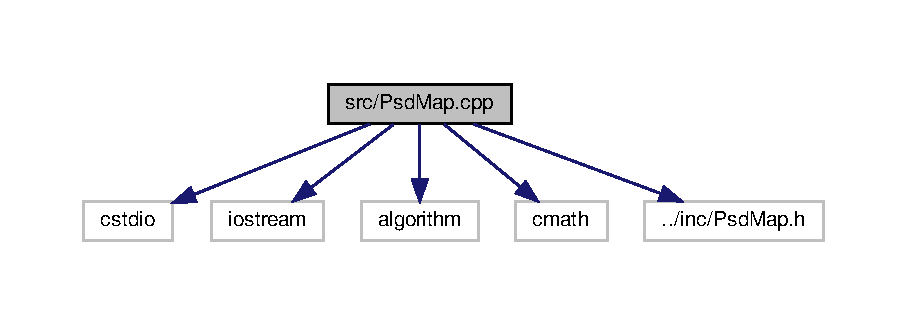
\includegraphics[width=350pt]{_psd_map_8cpp__incl}
\end{center}
\end{figure}
\subsection*{Macros}
\begin{DoxyCompactItemize}
\item 
\#define \hyperlink{_psd_map_8cpp_ab93fcdf0666a787a0fce927abd1c17b0}{P\+\_\+\+P\+S\+D\+\_\+\+Usage\+\_\+\+Active}~1
\end{DoxyCompactItemize}
\subsection*{Variables}
\begin{DoxyCompactItemize}
\item 
pthread\+\_\+mutex\+\_\+t \hyperlink{_psd_map_8cpp_a0e54b67a9bf300f936f9e747986659a4}{decoder\+Thread\+Mutex}
\item 
pthread\+\_\+mutex\+\_\+t \hyperlink{_psd_map_8cpp_aabb1d569e89cf787398ffc1a0a3b536c}{map\+Thread\+Mutex} = P\+T\+H\+R\+E\+A\+D\+\_\+\+M\+U\+T\+E\+X\+\_\+\+I\+N\+I\+T\+I\+A\+L\+I\+Z\+ER
\end{DoxyCompactItemize}


\subsection{Macro Definition Documentation}
\mbox{\Hypertarget{_psd_map_8cpp_ab93fcdf0666a787a0fce927abd1c17b0}\label{_psd_map_8cpp_ab93fcdf0666a787a0fce927abd1c17b0}} 
\index{Psd\+Map.\+cpp@{Psd\+Map.\+cpp}!P\+\_\+\+P\+S\+D\+\_\+\+Usage\+\_\+\+Active@{P\+\_\+\+P\+S\+D\+\_\+\+Usage\+\_\+\+Active}}
\index{P\+\_\+\+P\+S\+D\+\_\+\+Usage\+\_\+\+Active@{P\+\_\+\+P\+S\+D\+\_\+\+Usage\+\_\+\+Active}!Psd\+Map.\+cpp@{Psd\+Map.\+cpp}}
\subsubsection{\texorpdfstring{P\+\_\+\+P\+S\+D\+\_\+\+Usage\+\_\+\+Active}{P\_PSD\_Usage\_Active}}
{\footnotesize\ttfamily \#define P\+\_\+\+P\+S\+D\+\_\+\+Usage\+\_\+\+Active~1}



\subsection{Variable Documentation}
\mbox{\Hypertarget{_psd_map_8cpp_a0e54b67a9bf300f936f9e747986659a4}\label{_psd_map_8cpp_a0e54b67a9bf300f936f9e747986659a4}} 
\index{Psd\+Map.\+cpp@{Psd\+Map.\+cpp}!decoder\+Thread\+Mutex@{decoder\+Thread\+Mutex}}
\index{decoder\+Thread\+Mutex@{decoder\+Thread\+Mutex}!Psd\+Map.\+cpp@{Psd\+Map.\+cpp}}
\subsubsection{\texorpdfstring{decoder\+Thread\+Mutex}{decoderThreadMutex}}
{\footnotesize\ttfamily pthread\+\_\+mutex\+\_\+t decoder\+Thread\+Mutex}

\mbox{\Hypertarget{_psd_map_8cpp_aabb1d569e89cf787398ffc1a0a3b536c}\label{_psd_map_8cpp_aabb1d569e89cf787398ffc1a0a3b536c}} 
\index{Psd\+Map.\+cpp@{Psd\+Map.\+cpp}!map\+Thread\+Mutex@{map\+Thread\+Mutex}}
\index{map\+Thread\+Mutex@{map\+Thread\+Mutex}!Psd\+Map.\+cpp@{Psd\+Map.\+cpp}}
\subsubsection{\texorpdfstring{map\+Thread\+Mutex}{mapThreadMutex}}
{\footnotesize\ttfamily pthread\+\_\+mutex\+\_\+t map\+Thread\+Mutex = P\+T\+H\+R\+E\+A\+D\+\_\+\+M\+U\+T\+E\+X\+\_\+\+I\+N\+I\+T\+I\+A\+L\+I\+Z\+ER}


\hypertarget{_psd_map_8h}{}\section{src/\+Psd\+Map.h File Reference}
\label{_psd_map_8h}\index{src/\+Psd\+Map.\+h@{src/\+Psd\+Map.\+h}}
{\ttfamily \#include \char`\"{}Psd\+Message\+Decoder.\+h\char`\"{}}\newline
{\ttfamily \#include \char`\"{}Haversine.\+h\char`\"{}}\newline
Include dependency graph for Psd\+Map.\+h\+:\nopagebreak
\begin{figure}[H]
\begin{center}
\leavevmode
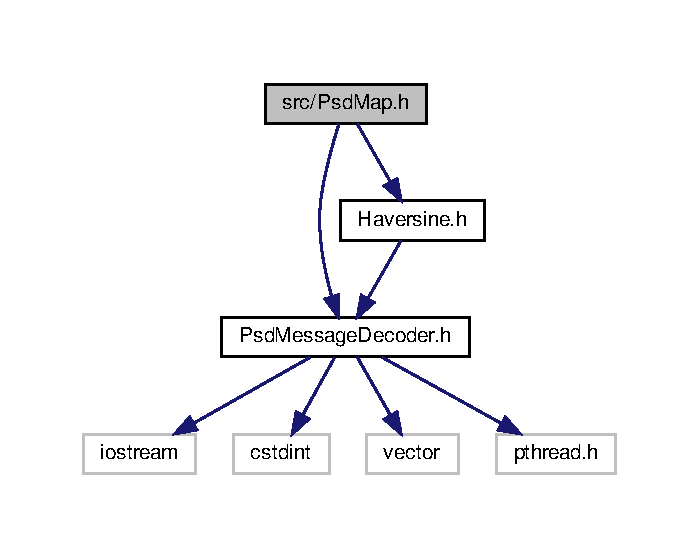
\includegraphics[width=336pt]{_psd_map_8h__incl}
\end{center}
\end{figure}
This graph shows which files directly or indirectly include this file\+:
\nopagebreak
\begin{figure}[H]
\begin{center}
\leavevmode
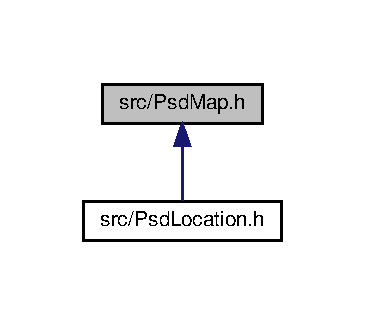
\includegraphics[width=175pt]{_psd_map_8h__dep__incl}
\end{center}
\end{figure}
\subsection*{Classes}
\begin{DoxyCompactItemize}
\item 
struct \hyperlink{struct_tree_node}{Tree\+Node}
\item 
class \hyperlink{class_psd_map}{Psd\+Map}
\end{DoxyCompactItemize}
\subsection*{Typedefs}
\begin{DoxyCompactItemize}
\item 
typedef struct \hyperlink{struct_tree_node}{Tree\+Node} \hyperlink{_psd_map_8h_aa2174826a70b13f771391e813b231770}{t\+Tree\+Node}
\end{DoxyCompactItemize}
\subsection*{Functions}
\begin{DoxyCompactItemize}
\item 
void $\ast$ \hyperlink{_psd_map_8h_ab233e13620a7fae2a5576ccf9d70f590}{Psd\+Map\+Run} (void $\ast$arg)
\end{DoxyCompactItemize}
\subsection*{Variables}
\begin{DoxyCompactItemize}
\item 
const double \hyperlink{_psd_map_8h_ab21be01fd4f091e93c4a3ba127af817c}{Max\+Road\+Error} = 7.\+0
\end{DoxyCompactItemize}


\subsection{Typedef Documentation}
\mbox{\Hypertarget{_psd_map_8h_aa2174826a70b13f771391e813b231770}\label{_psd_map_8h_aa2174826a70b13f771391e813b231770}} 
\index{Psd\+Map.\+h@{Psd\+Map.\+h}!t\+Tree\+Node@{t\+Tree\+Node}}
\index{t\+Tree\+Node@{t\+Tree\+Node}!Psd\+Map.\+h@{Psd\+Map.\+h}}
\subsubsection{\texorpdfstring{t\+Tree\+Node}{tTreeNode}}
{\footnotesize\ttfamily typedef struct \hyperlink{struct_tree_node}{Tree\+Node} \hyperlink{_psd_map_8h_aa2174826a70b13f771391e813b231770}{t\+Tree\+Node}}



\subsection{Function Documentation}
\mbox{\Hypertarget{_psd_map_8h_ab233e13620a7fae2a5576ccf9d70f590}\label{_psd_map_8h_ab233e13620a7fae2a5576ccf9d70f590}} 
\index{Psd\+Map.\+h@{Psd\+Map.\+h}!Psd\+Map\+Run@{Psd\+Map\+Run}}
\index{Psd\+Map\+Run@{Psd\+Map\+Run}!Psd\+Map.\+h@{Psd\+Map.\+h}}
\subsubsection{\texorpdfstring{Psd\+Map\+Run()}{PsdMapRun()}}
{\footnotesize\ttfamily void$\ast$ Psd\+Map\+Run (\begin{DoxyParamCaption}\item[{void $\ast$}]{arg }\end{DoxyParamCaption})}



\subsection{Variable Documentation}
\mbox{\Hypertarget{_psd_map_8h_ab21be01fd4f091e93c4a3ba127af817c}\label{_psd_map_8h_ab21be01fd4f091e93c4a3ba127af817c}} 
\index{Psd\+Map.\+h@{Psd\+Map.\+h}!Max\+Road\+Error@{Max\+Road\+Error}}
\index{Max\+Road\+Error@{Max\+Road\+Error}!Psd\+Map.\+h@{Psd\+Map.\+h}}
\subsubsection{\texorpdfstring{Max\+Road\+Error}{MaxRoadError}}
{\footnotesize\ttfamily const double Max\+Road\+Error = 7.\+0}


\hypertarget{_psd_message_decoder_8cpp}{}\section{src/\+Psd\+Message\+Decoder.cpp File Reference}
\label{_psd_message_decoder_8cpp}\index{src/\+Psd\+Message\+Decoder.\+cpp@{src/\+Psd\+Message\+Decoder.\+cpp}}
{\ttfamily \#include $<$cstdio$>$}\newline
{\ttfamily \#include $<$cstdlib$>$}\newline
{\ttfamily \#include $<$cstring$>$}\newline
{\ttfamily \#include $<$sys/types.\+h$>$}\newline
{\ttfamily \#include $<$cmath$>$}\newline
{\ttfamily \#include \char`\"{}../inc/\+Psd\+Message\+Decoder.\+h\char`\"{}}\newline
Include dependency graph for Psd\+Message\+Decoder.\+cpp\+:
\nopagebreak
\begin{figure}[H]
\begin{center}
\leavevmode
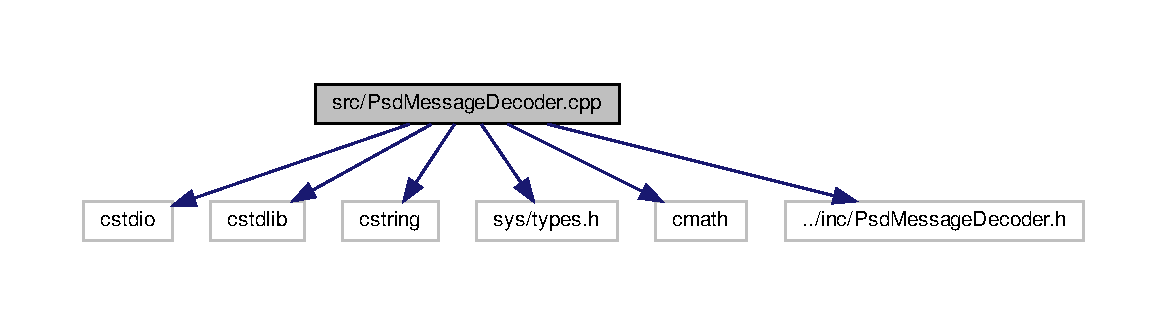
\includegraphics[width=350pt]{_psd_message_decoder_8cpp__incl}
\end{center}
\end{figure}
\subsection*{Macros}
\begin{DoxyCompactItemize}
\item 
\#define \hyperlink{_psd_message_decoder_8cpp_a63b46d5a8ecace201e68e55eb712fd72}{B\+R\+A\+N\+C\+H\+\_\+\+A\+N\+G\+L\+E\+\_\+\+S\+C\+A\+LE}~1.\+417323
\end{DoxyCompactItemize}
\subsection*{Variables}
\begin{DoxyCompactItemize}
\item 
pthread\+\_\+mutex\+\_\+t \hyperlink{_psd_message_decoder_8cpp_a0e54b67a9bf300f936f9e747986659a4}{decoder\+Thread\+Mutex} = P\+T\+H\+R\+E\+A\+D\+\_\+\+M\+U\+T\+E\+X\+\_\+\+I\+N\+I\+T\+I\+A\+L\+I\+Z\+ER
\end{DoxyCompactItemize}


\subsection{Macro Definition Documentation}
\mbox{\Hypertarget{_psd_message_decoder_8cpp_a63b46d5a8ecace201e68e55eb712fd72}\label{_psd_message_decoder_8cpp_a63b46d5a8ecace201e68e55eb712fd72}} 
\index{Psd\+Message\+Decoder.\+cpp@{Psd\+Message\+Decoder.\+cpp}!B\+R\+A\+N\+C\+H\+\_\+\+A\+N\+G\+L\+E\+\_\+\+S\+C\+A\+LE@{B\+R\+A\+N\+C\+H\+\_\+\+A\+N\+G\+L\+E\+\_\+\+S\+C\+A\+LE}}
\index{B\+R\+A\+N\+C\+H\+\_\+\+A\+N\+G\+L\+E\+\_\+\+S\+C\+A\+LE@{B\+R\+A\+N\+C\+H\+\_\+\+A\+N\+G\+L\+E\+\_\+\+S\+C\+A\+LE}!Psd\+Message\+Decoder.\+cpp@{Psd\+Message\+Decoder.\+cpp}}
\subsubsection{\texorpdfstring{B\+R\+A\+N\+C\+H\+\_\+\+A\+N\+G\+L\+E\+\_\+\+S\+C\+A\+LE}{BRANCH\_ANGLE\_SCALE}}
{\footnotesize\ttfamily \#define B\+R\+A\+N\+C\+H\+\_\+\+A\+N\+G\+L\+E\+\_\+\+S\+C\+A\+LE~1.\+417323}



\subsection{Variable Documentation}
\mbox{\Hypertarget{_psd_message_decoder_8cpp_a0e54b67a9bf300f936f9e747986659a4}\label{_psd_message_decoder_8cpp_a0e54b67a9bf300f936f9e747986659a4}} 
\index{Psd\+Message\+Decoder.\+cpp@{Psd\+Message\+Decoder.\+cpp}!decoder\+Thread\+Mutex@{decoder\+Thread\+Mutex}}
\index{decoder\+Thread\+Mutex@{decoder\+Thread\+Mutex}!Psd\+Message\+Decoder.\+cpp@{Psd\+Message\+Decoder.\+cpp}}
\subsubsection{\texorpdfstring{decoder\+Thread\+Mutex}{decoderThreadMutex}}
{\footnotesize\ttfamily pthread\+\_\+mutex\+\_\+t decoder\+Thread\+Mutex = P\+T\+H\+R\+E\+A\+D\+\_\+\+M\+U\+T\+E\+X\+\_\+\+I\+N\+I\+T\+I\+A\+L\+I\+Z\+ER}


\hypertarget{_psd_message_decoder_8h}{}\section{src/\+Psd\+Message\+Decoder.h File Reference}
\label{_psd_message_decoder_8h}\index{src/\+Psd\+Message\+Decoder.\+h@{src/\+Psd\+Message\+Decoder.\+h}}
{\ttfamily \#include $<$iostream$>$}\newline
{\ttfamily \#include $<$cstdint$>$}\newline
{\ttfamily \#include $<$vector$>$}\newline
{\ttfamily \#include $<$pthread.\+h$>$}\newline
Include dependency graph for Psd\+Message\+Decoder.\+h\+:\nopagebreak
\begin{figure}[H]
\begin{center}
\leavevmode
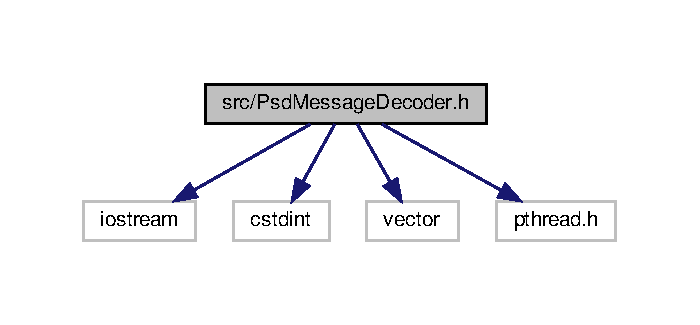
\includegraphics[width=336pt]{_psd_message_decoder_8h__incl}
\end{center}
\end{figure}
This graph shows which files directly or indirectly include this file\+:
\nopagebreak
\begin{figure}[H]
\begin{center}
\leavevmode
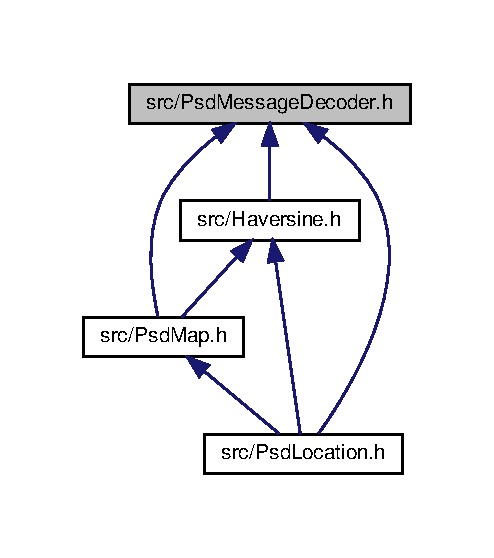
\includegraphics[width=237pt]{_psd_message_decoder_8h__dep__incl}
\end{center}
\end{figure}
\subsection*{Classes}
\begin{DoxyCompactItemize}
\item 
struct \hyperlink{struct_offset}{Offset}
\item 
struct \hyperlink{struct_coordinates}{Coordinates}
\item 
struct \hyperlink{struct_psd_map_data}{Psd\+Map\+Data}
\item 
struct \hyperlink{struct_self_segment}{Self\+Segment}
\item 
class \hyperlink{class_psd_message_decoder}{Psd\+Message\+Decoder}
\end{DoxyCompactItemize}
\subsection*{Typedefs}
\begin{DoxyCompactItemize}
\item 
typedef enum \hyperlink{_psd_message_decoder_8h_a4181d055fc39a45aa96e6f1c2c4e1000}{e\+Road\+Segment\+Class} \hyperlink{_psd_message_decoder_8h_a4f9adeb93dfc3dac7961fa97e890b1a5}{Road\+Segment\+Class}
\item 
typedef enum \hyperlink{_psd_message_decoder_8h_a21f903113ae6030410c94c4f7cc4b8ff}{e\+Psd04\+Road\+Class} \hyperlink{_psd_message_decoder_8h_a39044ce168ac526920bc721a8dc702b9}{Psd04\+Road\+Class}
\item 
typedef enum \hyperlink{_psd_message_decoder_8h_a8f791f18d2c949323fdbd44cf7147fb2}{Node\+Attribute} \hyperlink{_psd_message_decoder_8h_aa38e8413bd76f11962a364459c725e06}{e\+\_\+\+Node\+Attribute}
\item 
typedef enum \hyperlink{_psd_message_decoder_8h_afcf24267c16e7f9079b34b502b31dc12}{Pos\+Length\+Err} \hyperlink{_psd_message_decoder_8h_a954d216bca8cdfc325504c05bb6c4336}{e\+\_\+\+Pos\+Length\+Err}
\item 
typedef enum \hyperlink{_psd_message_decoder_8h_aac8c09b0eb267e00d3592c98792c2588}{Struct\+Separate} \hyperlink{_psd_message_decoder_8h_a2ba67cb465ee836b9ce8470f32577f21}{e\+\_\+\+Struct\+Separate}
\item 
typedef struct \hyperlink{struct_offset}{Offset} \hyperlink{_psd_message_decoder_8h_a7d8466510c49a8035fcf35b2949bea5a}{t\+Offset}
\item 
typedef struct \hyperlink{struct_coordinates}{Coordinates} \hyperlink{_psd_message_decoder_8h_a559ada7297c8c6c2337f9e233e73aeca}{t\+Coordinates}
\item 
typedef struct \hyperlink{struct_psd_map_data}{Psd\+Map\+Data} \hyperlink{_psd_message_decoder_8h_ad54e183dd7c544312c06d4bd6279ebdc}{t\+Psd\+Map\+Data}
\item 
typedef struct \hyperlink{struct_self_segment}{Self\+Segment} \hyperlink{_psd_message_decoder_8h_a6c858ba8556a68d900d0eca9dc406232}{t\+Self\+Segment}
\end{DoxyCompactItemize}
\subsection*{Enumerations}
\begin{DoxyCompactItemize}
\item 
enum \hyperlink{_psd_message_decoder_8h_a4181d055fc39a45aa96e6f1c2c4e1000}{e\+Road\+Segment\+Class} \{ \hyperlink{_psd_message_decoder_8h_a4181d055fc39a45aa96e6f1c2c4e1000ab9905873994d3154d09cc64e44b4af15}{Road\+Class\+\_\+\+Unkown} = 0, 
\hyperlink{_psd_message_decoder_8h_a4181d055fc39a45aa96e6f1c2c4e1000a8e0ecf498eb11d7848964d116d294b5b}{Road\+Class\+\_\+highway} = 1, 
\hyperlink{_psd_message_decoder_8h_a4181d055fc39a45aa96e6f1c2c4e1000a9f94ce51a3eb66debdce2f852f9e92df}{Road\+Class\+\_\+\+Non\+\_\+urban} = 2, 
\hyperlink{_psd_message_decoder_8h_a4181d055fc39a45aa96e6f1c2c4e1000a98f1668ab3701fc4ebf9e7944060aea5}{Road\+Class\+\_\+\+Urban} = 3
 \}
\item 
enum \hyperlink{_psd_message_decoder_8h_a21f903113ae6030410c94c4f7cc4b8ff}{e\+Psd04\+Road\+Class} \{ \newline
\hyperlink{_psd_message_decoder_8h_a21f903113ae6030410c94c4f7cc4b8ffadb4e856f9beef11cc5a4495e1388ed02}{Private\+Road} = 0, 
\hyperlink{_psd_message_decoder_8h_a21f903113ae6030410c94c4f7cc4b8ffaa425ea7f61c96f91080e6f5a95f71a4d}{Local\+Road} = 1, 
\hyperlink{_psd_message_decoder_8h_a21f903113ae6030410c94c4f7cc4b8ffa5baf9626106f6ef8ac298975c0e9265c}{County\+Road} = 2, 
\hyperlink{_psd_message_decoder_8h_a21f903113ae6030410c94c4f7cc4b8ffade5d711d362735c2b8495a05849407a4}{National\+Road} = 3, 
\newline
\hyperlink{_psd_message_decoder_8h_a21f903113ae6030410c94c4f7cc4b8ffae41117996b1be53d5dc8d7f701225e9c}{Provincial\+Road} = 4, 
\hyperlink{_psd_message_decoder_8h_a21f903113ae6030410c94c4f7cc4b8ffaaeb2c4111edc504ed3098b541db47221}{Expressway} = 5, 
\hyperlink{_psd_message_decoder_8h_a21f903113ae6030410c94c4f7cc4b8ffa1ff76aa808bb8209a13fcdbaf330587e}{Init} = 7
 \}
\item 
enum \hyperlink{_psd_message_decoder_8h_a8f791f18d2c949323fdbd44cf7147fb2}{Node\+Attribute} \{ \hyperlink{_psd_message_decoder_8h_a8f791f18d2c949323fdbd44cf7147fb2a5ed07430b29f8d6a7bdfbb5babee3fba}{Root\+Segment} = 1, 
\hyperlink{_psd_message_decoder_8h_a8f791f18d2c949323fdbd44cf7147fb2af865aeede76b8125cd74273093e8defd}{Parent\+Segment} = 2, 
\hyperlink{_psd_message_decoder_8h_a8f791f18d2c949323fdbd44cf7147fb2a69835f3a333258dbb50c1208db8d840a}{Cur\+Segment} = 3, 
\hyperlink{_psd_message_decoder_8h_a8f791f18d2c949323fdbd44cf7147fb2ad78b3980d73936a06dcabf1fe9c66bf5}{Child\+Segment} = 4
 \}
\item 
enum \hyperlink{_psd_message_decoder_8h_afcf24267c16e7f9079b34b502b31dc12}{Pos\+Length\+Err} \{ \newline
\hyperlink{_psd_message_decoder_8h_afcf24267c16e7f9079b34b502b31dc12a4a7cecb0d9a9445ceee18139782cd296}{Pos\+\_\+\+Init} = 0, 
\hyperlink{_psd_message_decoder_8h_afcf24267c16e7f9079b34b502b31dc12ad72fe6d28d20c27d908540807047b1c3}{Pos\+\_\+0m\+To2m} = 1, 
\hyperlink{_psd_message_decoder_8h_afcf24267c16e7f9079b34b502b31dc12a7b1a7fb12746ac3b2539845efde6d791}{Pos\+\_\+2m\+To5m} = 2, 
\hyperlink{_psd_message_decoder_8h_afcf24267c16e7f9079b34b502b31dc12ae41486b65e94f825256523f6a05d2294}{Pos\+\_\+5m\+To10m} = 3, 
\newline
\hyperlink{_psd_message_decoder_8h_afcf24267c16e7f9079b34b502b31dc12ac38053815bcac8b49938a9eec72f0bc1}{Pos\+\_\+10m\+To20m} = 4, 
\hyperlink{_psd_message_decoder_8h_afcf24267c16e7f9079b34b502b31dc12a7cf61a5ed51e4850fc3ee00941b10d24}{Pos\+\_\+20m\+To50m} = 5, 
\hyperlink{_psd_message_decoder_8h_afcf24267c16e7f9079b34b502b31dc12a4ef6931a0f205ebdeaeeafb688279757}{Over50m} = 6, 
\hyperlink{_psd_message_decoder_8h_afcf24267c16e7f9079b34b502b31dc12aecb43e8842e8cf4125156b93f972c022}{Off\+Road} = 7
 \}
\item 
enum \hyperlink{_psd_message_decoder_8h_aac8c09b0eb267e00d3592c98792c2588}{Struct\+Separate} \{ \hyperlink{_psd_message_decoder_8h_aac8c09b0eb267e00d3592c98792c2588ab1bc2d90e57ef779aff20ad87dc522cb}{No\+Seperation} = 0, 
\hyperlink{_psd_message_decoder_8h_aac8c09b0eb267e00d3592c98792c2588a6b158ae4252a826b81386eb679a77914}{Structural\+Seperation} = 1, 
\hyperlink{_psd_message_decoder_8h_aac8c09b0eb267e00d3592c98792c2588a8a858a380fb62c8651b25c5d3f4e68be}{Seperation\+But\+No\+Structural} = 2, 
\hyperlink{_psd_message_decoder_8h_aac8c09b0eb267e00d3592c98792c2588aed3b39cbaec7041b9e14a89928a29dca}{No\+Info} = 3
 \}
\end{DoxyCompactItemize}
\subsection*{Functions}
\begin{DoxyCompactItemize}
\item 
void $\ast$ \hyperlink{_psd_message_decoder_8h_a99afa19c7e74376d95279fd72d4febef}{Psd\+Message\+Decoder\+Run} (void $\ast$arg)
\end{DoxyCompactItemize}


\subsection{Typedef Documentation}
\mbox{\Hypertarget{_psd_message_decoder_8h_aa38e8413bd76f11962a364459c725e06}\label{_psd_message_decoder_8h_aa38e8413bd76f11962a364459c725e06}} 
\index{Psd\+Message\+Decoder.\+h@{Psd\+Message\+Decoder.\+h}!e\+\_\+\+Node\+Attribute@{e\+\_\+\+Node\+Attribute}}
\index{e\+\_\+\+Node\+Attribute@{e\+\_\+\+Node\+Attribute}!Psd\+Message\+Decoder.\+h@{Psd\+Message\+Decoder.\+h}}
\subsubsection{\texorpdfstring{e\+\_\+\+Node\+Attribute}{e\_NodeAttribute}}
{\footnotesize\ttfamily typedef enum \hyperlink{_psd_message_decoder_8h_a8f791f18d2c949323fdbd44cf7147fb2}{Node\+Attribute} \hyperlink{_psd_message_decoder_8h_aa38e8413bd76f11962a364459c725e06}{e\+\_\+\+Node\+Attribute}}

\mbox{\Hypertarget{_psd_message_decoder_8h_a954d216bca8cdfc325504c05bb6c4336}\label{_psd_message_decoder_8h_a954d216bca8cdfc325504c05bb6c4336}} 
\index{Psd\+Message\+Decoder.\+h@{Psd\+Message\+Decoder.\+h}!e\+\_\+\+Pos\+Length\+Err@{e\+\_\+\+Pos\+Length\+Err}}
\index{e\+\_\+\+Pos\+Length\+Err@{e\+\_\+\+Pos\+Length\+Err}!Psd\+Message\+Decoder.\+h@{Psd\+Message\+Decoder.\+h}}
\subsubsection{\texorpdfstring{e\+\_\+\+Pos\+Length\+Err}{e\_PosLengthErr}}
{\footnotesize\ttfamily typedef enum \hyperlink{_psd_message_decoder_8h_afcf24267c16e7f9079b34b502b31dc12}{Pos\+Length\+Err} \hyperlink{_psd_message_decoder_8h_a954d216bca8cdfc325504c05bb6c4336}{e\+\_\+\+Pos\+Length\+Err}}

\mbox{\Hypertarget{_psd_message_decoder_8h_a2ba67cb465ee836b9ce8470f32577f21}\label{_psd_message_decoder_8h_a2ba67cb465ee836b9ce8470f32577f21}} 
\index{Psd\+Message\+Decoder.\+h@{Psd\+Message\+Decoder.\+h}!e\+\_\+\+Struct\+Separate@{e\+\_\+\+Struct\+Separate}}
\index{e\+\_\+\+Struct\+Separate@{e\+\_\+\+Struct\+Separate}!Psd\+Message\+Decoder.\+h@{Psd\+Message\+Decoder.\+h}}
\subsubsection{\texorpdfstring{e\+\_\+\+Struct\+Separate}{e\_StructSeparate}}
{\footnotesize\ttfamily typedef enum \hyperlink{_psd_message_decoder_8h_aac8c09b0eb267e00d3592c98792c2588}{Struct\+Separate} \hyperlink{_psd_message_decoder_8h_a2ba67cb465ee836b9ce8470f32577f21}{e\+\_\+\+Struct\+Separate}}

\mbox{\Hypertarget{_psd_message_decoder_8h_a39044ce168ac526920bc721a8dc702b9}\label{_psd_message_decoder_8h_a39044ce168ac526920bc721a8dc702b9}} 
\index{Psd\+Message\+Decoder.\+h@{Psd\+Message\+Decoder.\+h}!Psd04\+Road\+Class@{Psd04\+Road\+Class}}
\index{Psd04\+Road\+Class@{Psd04\+Road\+Class}!Psd\+Message\+Decoder.\+h@{Psd\+Message\+Decoder.\+h}}
\subsubsection{\texorpdfstring{Psd04\+Road\+Class}{Psd04RoadClass}}
{\footnotesize\ttfamily typedef enum \hyperlink{_psd_message_decoder_8h_a21f903113ae6030410c94c4f7cc4b8ff}{e\+Psd04\+Road\+Class} \hyperlink{_psd_message_decoder_8h_a39044ce168ac526920bc721a8dc702b9}{Psd04\+Road\+Class}}

\mbox{\Hypertarget{_psd_message_decoder_8h_a4f9adeb93dfc3dac7961fa97e890b1a5}\label{_psd_message_decoder_8h_a4f9adeb93dfc3dac7961fa97e890b1a5}} 
\index{Psd\+Message\+Decoder.\+h@{Psd\+Message\+Decoder.\+h}!Road\+Segment\+Class@{Road\+Segment\+Class}}
\index{Road\+Segment\+Class@{Road\+Segment\+Class}!Psd\+Message\+Decoder.\+h@{Psd\+Message\+Decoder.\+h}}
\subsubsection{\texorpdfstring{Road\+Segment\+Class}{RoadSegmentClass}}
{\footnotesize\ttfamily typedef enum \hyperlink{_psd_message_decoder_8h_a4181d055fc39a45aa96e6f1c2c4e1000}{e\+Road\+Segment\+Class} \hyperlink{_psd_message_decoder_8h_a4f9adeb93dfc3dac7961fa97e890b1a5}{Road\+Segment\+Class}}

\mbox{\Hypertarget{_psd_message_decoder_8h_a559ada7297c8c6c2337f9e233e73aeca}\label{_psd_message_decoder_8h_a559ada7297c8c6c2337f9e233e73aeca}} 
\index{Psd\+Message\+Decoder.\+h@{Psd\+Message\+Decoder.\+h}!t\+Coordinates@{t\+Coordinates}}
\index{t\+Coordinates@{t\+Coordinates}!Psd\+Message\+Decoder.\+h@{Psd\+Message\+Decoder.\+h}}
\subsubsection{\texorpdfstring{t\+Coordinates}{tCoordinates}}
{\footnotesize\ttfamily typedef struct \hyperlink{struct_coordinates}{Coordinates} \hyperlink{_psd_message_decoder_8h_a559ada7297c8c6c2337f9e233e73aeca}{t\+Coordinates}}

\mbox{\Hypertarget{_psd_message_decoder_8h_a7d8466510c49a8035fcf35b2949bea5a}\label{_psd_message_decoder_8h_a7d8466510c49a8035fcf35b2949bea5a}} 
\index{Psd\+Message\+Decoder.\+h@{Psd\+Message\+Decoder.\+h}!t\+Offset@{t\+Offset}}
\index{t\+Offset@{t\+Offset}!Psd\+Message\+Decoder.\+h@{Psd\+Message\+Decoder.\+h}}
\subsubsection{\texorpdfstring{t\+Offset}{tOffset}}
{\footnotesize\ttfamily typedef struct \hyperlink{struct_offset}{Offset} \hyperlink{_psd_message_decoder_8h_a7d8466510c49a8035fcf35b2949bea5a}{t\+Offset}}

\mbox{\Hypertarget{_psd_message_decoder_8h_ad54e183dd7c544312c06d4bd6279ebdc}\label{_psd_message_decoder_8h_ad54e183dd7c544312c06d4bd6279ebdc}} 
\index{Psd\+Message\+Decoder.\+h@{Psd\+Message\+Decoder.\+h}!t\+Psd\+Map\+Data@{t\+Psd\+Map\+Data}}
\index{t\+Psd\+Map\+Data@{t\+Psd\+Map\+Data}!Psd\+Message\+Decoder.\+h@{Psd\+Message\+Decoder.\+h}}
\subsubsection{\texorpdfstring{t\+Psd\+Map\+Data}{tPsdMapData}}
{\footnotesize\ttfamily typedef struct \hyperlink{struct_psd_map_data}{Psd\+Map\+Data} \hyperlink{_psd_message_decoder_8h_ad54e183dd7c544312c06d4bd6279ebdc}{t\+Psd\+Map\+Data}}

\mbox{\Hypertarget{_psd_message_decoder_8h_a6c858ba8556a68d900d0eca9dc406232}\label{_psd_message_decoder_8h_a6c858ba8556a68d900d0eca9dc406232}} 
\index{Psd\+Message\+Decoder.\+h@{Psd\+Message\+Decoder.\+h}!t\+Self\+Segment@{t\+Self\+Segment}}
\index{t\+Self\+Segment@{t\+Self\+Segment}!Psd\+Message\+Decoder.\+h@{Psd\+Message\+Decoder.\+h}}
\subsubsection{\texorpdfstring{t\+Self\+Segment}{tSelfSegment}}
{\footnotesize\ttfamily typedef struct \hyperlink{struct_self_segment}{Self\+Segment} \hyperlink{_psd_message_decoder_8h_a6c858ba8556a68d900d0eca9dc406232}{t\+Self\+Segment}}



\subsection{Enumeration Type Documentation}
\mbox{\Hypertarget{_psd_message_decoder_8h_a21f903113ae6030410c94c4f7cc4b8ff}\label{_psd_message_decoder_8h_a21f903113ae6030410c94c4f7cc4b8ff}} 
\index{Psd\+Message\+Decoder.\+h@{Psd\+Message\+Decoder.\+h}!e\+Psd04\+Road\+Class@{e\+Psd04\+Road\+Class}}
\index{e\+Psd04\+Road\+Class@{e\+Psd04\+Road\+Class}!Psd\+Message\+Decoder.\+h@{Psd\+Message\+Decoder.\+h}}
\subsubsection{\texorpdfstring{e\+Psd04\+Road\+Class}{ePsd04RoadClass}}
{\footnotesize\ttfamily enum \hyperlink{_psd_message_decoder_8h_a21f903113ae6030410c94c4f7cc4b8ff}{e\+Psd04\+Road\+Class}}

\begin{DoxyEnumFields}{Enumerator}
\raisebox{\heightof{T}}[0pt][0pt]{\index{Private\+Road@{Private\+Road}!Psd\+Message\+Decoder.\+h@{Psd\+Message\+Decoder.\+h}}\index{Psd\+Message\+Decoder.\+h@{Psd\+Message\+Decoder.\+h}!Private\+Road@{Private\+Road}}}\mbox{\Hypertarget{_psd_message_decoder_8h_a21f903113ae6030410c94c4f7cc4b8ffadb4e856f9beef11cc5a4495e1388ed02}\label{_psd_message_decoder_8h_a21f903113ae6030410c94c4f7cc4b8ffadb4e856f9beef11cc5a4495e1388ed02}} 
Private\+Road&\\
\hline

\raisebox{\heightof{T}}[0pt][0pt]{\index{Local\+Road@{Local\+Road}!Psd\+Message\+Decoder.\+h@{Psd\+Message\+Decoder.\+h}}\index{Psd\+Message\+Decoder.\+h@{Psd\+Message\+Decoder.\+h}!Local\+Road@{Local\+Road}}}\mbox{\Hypertarget{_psd_message_decoder_8h_a21f903113ae6030410c94c4f7cc4b8ffaa425ea7f61c96f91080e6f5a95f71a4d}\label{_psd_message_decoder_8h_a21f903113ae6030410c94c4f7cc4b8ffaa425ea7f61c96f91080e6f5a95f71a4d}} 
Local\+Road&\\
\hline

\raisebox{\heightof{T}}[0pt][0pt]{\index{County\+Road@{County\+Road}!Psd\+Message\+Decoder.\+h@{Psd\+Message\+Decoder.\+h}}\index{Psd\+Message\+Decoder.\+h@{Psd\+Message\+Decoder.\+h}!County\+Road@{County\+Road}}}\mbox{\Hypertarget{_psd_message_decoder_8h_a21f903113ae6030410c94c4f7cc4b8ffa5baf9626106f6ef8ac298975c0e9265c}\label{_psd_message_decoder_8h_a21f903113ae6030410c94c4f7cc4b8ffa5baf9626106f6ef8ac298975c0e9265c}} 
County\+Road&\\
\hline

\raisebox{\heightof{T}}[0pt][0pt]{\index{National\+Road@{National\+Road}!Psd\+Message\+Decoder.\+h@{Psd\+Message\+Decoder.\+h}}\index{Psd\+Message\+Decoder.\+h@{Psd\+Message\+Decoder.\+h}!National\+Road@{National\+Road}}}\mbox{\Hypertarget{_psd_message_decoder_8h_a21f903113ae6030410c94c4f7cc4b8ffade5d711d362735c2b8495a05849407a4}\label{_psd_message_decoder_8h_a21f903113ae6030410c94c4f7cc4b8ffade5d711d362735c2b8495a05849407a4}} 
National\+Road&\\
\hline

\raisebox{\heightof{T}}[0pt][0pt]{\index{Provincial\+Road@{Provincial\+Road}!Psd\+Message\+Decoder.\+h@{Psd\+Message\+Decoder.\+h}}\index{Psd\+Message\+Decoder.\+h@{Psd\+Message\+Decoder.\+h}!Provincial\+Road@{Provincial\+Road}}}\mbox{\Hypertarget{_psd_message_decoder_8h_a21f903113ae6030410c94c4f7cc4b8ffae41117996b1be53d5dc8d7f701225e9c}\label{_psd_message_decoder_8h_a21f903113ae6030410c94c4f7cc4b8ffae41117996b1be53d5dc8d7f701225e9c}} 
Provincial\+Road&\\
\hline

\raisebox{\heightof{T}}[0pt][0pt]{\index{Expressway@{Expressway}!Psd\+Message\+Decoder.\+h@{Psd\+Message\+Decoder.\+h}}\index{Psd\+Message\+Decoder.\+h@{Psd\+Message\+Decoder.\+h}!Expressway@{Expressway}}}\mbox{\Hypertarget{_psd_message_decoder_8h_a21f903113ae6030410c94c4f7cc4b8ffaaeb2c4111edc504ed3098b541db47221}\label{_psd_message_decoder_8h_a21f903113ae6030410c94c4f7cc4b8ffaaeb2c4111edc504ed3098b541db47221}} 
Expressway&\\
\hline

\raisebox{\heightof{T}}[0pt][0pt]{\index{Init@{Init}!Psd\+Message\+Decoder.\+h@{Psd\+Message\+Decoder.\+h}}\index{Psd\+Message\+Decoder.\+h@{Psd\+Message\+Decoder.\+h}!Init@{Init}}}\mbox{\Hypertarget{_psd_message_decoder_8h_a21f903113ae6030410c94c4f7cc4b8ffa1ff76aa808bb8209a13fcdbaf330587e}\label{_psd_message_decoder_8h_a21f903113ae6030410c94c4f7cc4b8ffa1ff76aa808bb8209a13fcdbaf330587e}} 
Init&\\
\hline

\end{DoxyEnumFields}
\mbox{\Hypertarget{_psd_message_decoder_8h_a4181d055fc39a45aa96e6f1c2c4e1000}\label{_psd_message_decoder_8h_a4181d055fc39a45aa96e6f1c2c4e1000}} 
\index{Psd\+Message\+Decoder.\+h@{Psd\+Message\+Decoder.\+h}!e\+Road\+Segment\+Class@{e\+Road\+Segment\+Class}}
\index{e\+Road\+Segment\+Class@{e\+Road\+Segment\+Class}!Psd\+Message\+Decoder.\+h@{Psd\+Message\+Decoder.\+h}}
\subsubsection{\texorpdfstring{e\+Road\+Segment\+Class}{eRoadSegmentClass}}
{\footnotesize\ttfamily enum \hyperlink{_psd_message_decoder_8h_a4181d055fc39a45aa96e6f1c2c4e1000}{e\+Road\+Segment\+Class}}

\begin{DoxyEnumFields}{Enumerator}
\raisebox{\heightof{T}}[0pt][0pt]{\index{Road\+Class\+\_\+\+Unkown@{Road\+Class\+\_\+\+Unkown}!Psd\+Message\+Decoder.\+h@{Psd\+Message\+Decoder.\+h}}\index{Psd\+Message\+Decoder.\+h@{Psd\+Message\+Decoder.\+h}!Road\+Class\+\_\+\+Unkown@{Road\+Class\+\_\+\+Unkown}}}\mbox{\Hypertarget{_psd_message_decoder_8h_a4181d055fc39a45aa96e6f1c2c4e1000ab9905873994d3154d09cc64e44b4af15}\label{_psd_message_decoder_8h_a4181d055fc39a45aa96e6f1c2c4e1000ab9905873994d3154d09cc64e44b4af15}} 
Road\+Class\+\_\+\+Unkown&\\
\hline

\raisebox{\heightof{T}}[0pt][0pt]{\index{Road\+Class\+\_\+highway@{Road\+Class\+\_\+highway}!Psd\+Message\+Decoder.\+h@{Psd\+Message\+Decoder.\+h}}\index{Psd\+Message\+Decoder.\+h@{Psd\+Message\+Decoder.\+h}!Road\+Class\+\_\+highway@{Road\+Class\+\_\+highway}}}\mbox{\Hypertarget{_psd_message_decoder_8h_a4181d055fc39a45aa96e6f1c2c4e1000a8e0ecf498eb11d7848964d116d294b5b}\label{_psd_message_decoder_8h_a4181d055fc39a45aa96e6f1c2c4e1000a8e0ecf498eb11d7848964d116d294b5b}} 
Road\+Class\+\_\+highway&\\
\hline

\raisebox{\heightof{T}}[0pt][0pt]{\index{Road\+Class\+\_\+\+Non\+\_\+urban@{Road\+Class\+\_\+\+Non\+\_\+urban}!Psd\+Message\+Decoder.\+h@{Psd\+Message\+Decoder.\+h}}\index{Psd\+Message\+Decoder.\+h@{Psd\+Message\+Decoder.\+h}!Road\+Class\+\_\+\+Non\+\_\+urban@{Road\+Class\+\_\+\+Non\+\_\+urban}}}\mbox{\Hypertarget{_psd_message_decoder_8h_a4181d055fc39a45aa96e6f1c2c4e1000a9f94ce51a3eb66debdce2f852f9e92df}\label{_psd_message_decoder_8h_a4181d055fc39a45aa96e6f1c2c4e1000a9f94ce51a3eb66debdce2f852f9e92df}} 
Road\+Class\+\_\+\+Non\+\_\+urban&\\
\hline

\raisebox{\heightof{T}}[0pt][0pt]{\index{Road\+Class\+\_\+\+Urban@{Road\+Class\+\_\+\+Urban}!Psd\+Message\+Decoder.\+h@{Psd\+Message\+Decoder.\+h}}\index{Psd\+Message\+Decoder.\+h@{Psd\+Message\+Decoder.\+h}!Road\+Class\+\_\+\+Urban@{Road\+Class\+\_\+\+Urban}}}\mbox{\Hypertarget{_psd_message_decoder_8h_a4181d055fc39a45aa96e6f1c2c4e1000a98f1668ab3701fc4ebf9e7944060aea5}\label{_psd_message_decoder_8h_a4181d055fc39a45aa96e6f1c2c4e1000a98f1668ab3701fc4ebf9e7944060aea5}} 
Road\+Class\+\_\+\+Urban&\\
\hline

\end{DoxyEnumFields}
\mbox{\Hypertarget{_psd_message_decoder_8h_a8f791f18d2c949323fdbd44cf7147fb2}\label{_psd_message_decoder_8h_a8f791f18d2c949323fdbd44cf7147fb2}} 
\index{Psd\+Message\+Decoder.\+h@{Psd\+Message\+Decoder.\+h}!Node\+Attribute@{Node\+Attribute}}
\index{Node\+Attribute@{Node\+Attribute}!Psd\+Message\+Decoder.\+h@{Psd\+Message\+Decoder.\+h}}
\subsubsection{\texorpdfstring{Node\+Attribute}{NodeAttribute}}
{\footnotesize\ttfamily enum \hyperlink{_psd_message_decoder_8h_a8f791f18d2c949323fdbd44cf7147fb2}{Node\+Attribute}}

\begin{DoxyEnumFields}{Enumerator}
\raisebox{\heightof{T}}[0pt][0pt]{\index{Root\+Segment@{Root\+Segment}!Psd\+Message\+Decoder.\+h@{Psd\+Message\+Decoder.\+h}}\index{Psd\+Message\+Decoder.\+h@{Psd\+Message\+Decoder.\+h}!Root\+Segment@{Root\+Segment}}}\mbox{\Hypertarget{_psd_message_decoder_8h_a8f791f18d2c949323fdbd44cf7147fb2a5ed07430b29f8d6a7bdfbb5babee3fba}\label{_psd_message_decoder_8h_a8f791f18d2c949323fdbd44cf7147fb2a5ed07430b29f8d6a7bdfbb5babee3fba}} 
Root\+Segment&\\
\hline

\raisebox{\heightof{T}}[0pt][0pt]{\index{Parent\+Segment@{Parent\+Segment}!Psd\+Message\+Decoder.\+h@{Psd\+Message\+Decoder.\+h}}\index{Psd\+Message\+Decoder.\+h@{Psd\+Message\+Decoder.\+h}!Parent\+Segment@{Parent\+Segment}}}\mbox{\Hypertarget{_psd_message_decoder_8h_a8f791f18d2c949323fdbd44cf7147fb2af865aeede76b8125cd74273093e8defd}\label{_psd_message_decoder_8h_a8f791f18d2c949323fdbd44cf7147fb2af865aeede76b8125cd74273093e8defd}} 
Parent\+Segment&\\
\hline

\raisebox{\heightof{T}}[0pt][0pt]{\index{Cur\+Segment@{Cur\+Segment}!Psd\+Message\+Decoder.\+h@{Psd\+Message\+Decoder.\+h}}\index{Psd\+Message\+Decoder.\+h@{Psd\+Message\+Decoder.\+h}!Cur\+Segment@{Cur\+Segment}}}\mbox{\Hypertarget{_psd_message_decoder_8h_a8f791f18d2c949323fdbd44cf7147fb2a69835f3a333258dbb50c1208db8d840a}\label{_psd_message_decoder_8h_a8f791f18d2c949323fdbd44cf7147fb2a69835f3a333258dbb50c1208db8d840a}} 
Cur\+Segment&\\
\hline

\raisebox{\heightof{T}}[0pt][0pt]{\index{Child\+Segment@{Child\+Segment}!Psd\+Message\+Decoder.\+h@{Psd\+Message\+Decoder.\+h}}\index{Psd\+Message\+Decoder.\+h@{Psd\+Message\+Decoder.\+h}!Child\+Segment@{Child\+Segment}}}\mbox{\Hypertarget{_psd_message_decoder_8h_a8f791f18d2c949323fdbd44cf7147fb2ad78b3980d73936a06dcabf1fe9c66bf5}\label{_psd_message_decoder_8h_a8f791f18d2c949323fdbd44cf7147fb2ad78b3980d73936a06dcabf1fe9c66bf5}} 
Child\+Segment&\\
\hline

\end{DoxyEnumFields}
\mbox{\Hypertarget{_psd_message_decoder_8h_afcf24267c16e7f9079b34b502b31dc12}\label{_psd_message_decoder_8h_afcf24267c16e7f9079b34b502b31dc12}} 
\index{Psd\+Message\+Decoder.\+h@{Psd\+Message\+Decoder.\+h}!Pos\+Length\+Err@{Pos\+Length\+Err}}
\index{Pos\+Length\+Err@{Pos\+Length\+Err}!Psd\+Message\+Decoder.\+h@{Psd\+Message\+Decoder.\+h}}
\subsubsection{\texorpdfstring{Pos\+Length\+Err}{PosLengthErr}}
{\footnotesize\ttfamily enum \hyperlink{_psd_message_decoder_8h_afcf24267c16e7f9079b34b502b31dc12}{Pos\+Length\+Err}}

\begin{DoxyEnumFields}{Enumerator}
\raisebox{\heightof{T}}[0pt][0pt]{\index{Pos\+\_\+\+Init@{Pos\+\_\+\+Init}!Psd\+Message\+Decoder.\+h@{Psd\+Message\+Decoder.\+h}}\index{Psd\+Message\+Decoder.\+h@{Psd\+Message\+Decoder.\+h}!Pos\+\_\+\+Init@{Pos\+\_\+\+Init}}}\mbox{\Hypertarget{_psd_message_decoder_8h_afcf24267c16e7f9079b34b502b31dc12a4a7cecb0d9a9445ceee18139782cd296}\label{_psd_message_decoder_8h_afcf24267c16e7f9079b34b502b31dc12a4a7cecb0d9a9445ceee18139782cd296}} 
Pos\+\_\+\+Init&\\
\hline

\raisebox{\heightof{T}}[0pt][0pt]{\index{Pos\+\_\+0m\+To2m@{Pos\+\_\+0m\+To2m}!Psd\+Message\+Decoder.\+h@{Psd\+Message\+Decoder.\+h}}\index{Psd\+Message\+Decoder.\+h@{Psd\+Message\+Decoder.\+h}!Pos\+\_\+0m\+To2m@{Pos\+\_\+0m\+To2m}}}\mbox{\Hypertarget{_psd_message_decoder_8h_afcf24267c16e7f9079b34b502b31dc12ad72fe6d28d20c27d908540807047b1c3}\label{_psd_message_decoder_8h_afcf24267c16e7f9079b34b502b31dc12ad72fe6d28d20c27d908540807047b1c3}} 
Pos\+\_\+0m\+To2m&\\
\hline

\raisebox{\heightof{T}}[0pt][0pt]{\index{Pos\+\_\+2m\+To5m@{Pos\+\_\+2m\+To5m}!Psd\+Message\+Decoder.\+h@{Psd\+Message\+Decoder.\+h}}\index{Psd\+Message\+Decoder.\+h@{Psd\+Message\+Decoder.\+h}!Pos\+\_\+2m\+To5m@{Pos\+\_\+2m\+To5m}}}\mbox{\Hypertarget{_psd_message_decoder_8h_afcf24267c16e7f9079b34b502b31dc12a7b1a7fb12746ac3b2539845efde6d791}\label{_psd_message_decoder_8h_afcf24267c16e7f9079b34b502b31dc12a7b1a7fb12746ac3b2539845efde6d791}} 
Pos\+\_\+2m\+To5m&\\
\hline

\raisebox{\heightof{T}}[0pt][0pt]{\index{Pos\+\_\+5m\+To10m@{Pos\+\_\+5m\+To10m}!Psd\+Message\+Decoder.\+h@{Psd\+Message\+Decoder.\+h}}\index{Psd\+Message\+Decoder.\+h@{Psd\+Message\+Decoder.\+h}!Pos\+\_\+5m\+To10m@{Pos\+\_\+5m\+To10m}}}\mbox{\Hypertarget{_psd_message_decoder_8h_afcf24267c16e7f9079b34b502b31dc12ae41486b65e94f825256523f6a05d2294}\label{_psd_message_decoder_8h_afcf24267c16e7f9079b34b502b31dc12ae41486b65e94f825256523f6a05d2294}} 
Pos\+\_\+5m\+To10m&\\
\hline

\raisebox{\heightof{T}}[0pt][0pt]{\index{Pos\+\_\+10m\+To20m@{Pos\+\_\+10m\+To20m}!Psd\+Message\+Decoder.\+h@{Psd\+Message\+Decoder.\+h}}\index{Psd\+Message\+Decoder.\+h@{Psd\+Message\+Decoder.\+h}!Pos\+\_\+10m\+To20m@{Pos\+\_\+10m\+To20m}}}\mbox{\Hypertarget{_psd_message_decoder_8h_afcf24267c16e7f9079b34b502b31dc12ac38053815bcac8b49938a9eec72f0bc1}\label{_psd_message_decoder_8h_afcf24267c16e7f9079b34b502b31dc12ac38053815bcac8b49938a9eec72f0bc1}} 
Pos\+\_\+10m\+To20m&\\
\hline

\raisebox{\heightof{T}}[0pt][0pt]{\index{Pos\+\_\+20m\+To50m@{Pos\+\_\+20m\+To50m}!Psd\+Message\+Decoder.\+h@{Psd\+Message\+Decoder.\+h}}\index{Psd\+Message\+Decoder.\+h@{Psd\+Message\+Decoder.\+h}!Pos\+\_\+20m\+To50m@{Pos\+\_\+20m\+To50m}}}\mbox{\Hypertarget{_psd_message_decoder_8h_afcf24267c16e7f9079b34b502b31dc12a7cf61a5ed51e4850fc3ee00941b10d24}\label{_psd_message_decoder_8h_afcf24267c16e7f9079b34b502b31dc12a7cf61a5ed51e4850fc3ee00941b10d24}} 
Pos\+\_\+20m\+To50m&\\
\hline

\raisebox{\heightof{T}}[0pt][0pt]{\index{Over50m@{Over50m}!Psd\+Message\+Decoder.\+h@{Psd\+Message\+Decoder.\+h}}\index{Psd\+Message\+Decoder.\+h@{Psd\+Message\+Decoder.\+h}!Over50m@{Over50m}}}\mbox{\Hypertarget{_psd_message_decoder_8h_afcf24267c16e7f9079b34b502b31dc12a4ef6931a0f205ebdeaeeafb688279757}\label{_psd_message_decoder_8h_afcf24267c16e7f9079b34b502b31dc12a4ef6931a0f205ebdeaeeafb688279757}} 
Over50m&\\
\hline

\raisebox{\heightof{T}}[0pt][0pt]{\index{Off\+Road@{Off\+Road}!Psd\+Message\+Decoder.\+h@{Psd\+Message\+Decoder.\+h}}\index{Psd\+Message\+Decoder.\+h@{Psd\+Message\+Decoder.\+h}!Off\+Road@{Off\+Road}}}\mbox{\Hypertarget{_psd_message_decoder_8h_afcf24267c16e7f9079b34b502b31dc12aecb43e8842e8cf4125156b93f972c022}\label{_psd_message_decoder_8h_afcf24267c16e7f9079b34b502b31dc12aecb43e8842e8cf4125156b93f972c022}} 
Off\+Road&\\
\hline

\end{DoxyEnumFields}
\mbox{\Hypertarget{_psd_message_decoder_8h_aac8c09b0eb267e00d3592c98792c2588}\label{_psd_message_decoder_8h_aac8c09b0eb267e00d3592c98792c2588}} 
\index{Psd\+Message\+Decoder.\+h@{Psd\+Message\+Decoder.\+h}!Struct\+Separate@{Struct\+Separate}}
\index{Struct\+Separate@{Struct\+Separate}!Psd\+Message\+Decoder.\+h@{Psd\+Message\+Decoder.\+h}}
\subsubsection{\texorpdfstring{Struct\+Separate}{StructSeparate}}
{\footnotesize\ttfamily enum \hyperlink{_psd_message_decoder_8h_aac8c09b0eb267e00d3592c98792c2588}{Struct\+Separate}}

\begin{DoxyEnumFields}{Enumerator}
\raisebox{\heightof{T}}[0pt][0pt]{\index{No\+Seperation@{No\+Seperation}!Psd\+Message\+Decoder.\+h@{Psd\+Message\+Decoder.\+h}}\index{Psd\+Message\+Decoder.\+h@{Psd\+Message\+Decoder.\+h}!No\+Seperation@{No\+Seperation}}}\mbox{\Hypertarget{_psd_message_decoder_8h_aac8c09b0eb267e00d3592c98792c2588ab1bc2d90e57ef779aff20ad87dc522cb}\label{_psd_message_decoder_8h_aac8c09b0eb267e00d3592c98792c2588ab1bc2d90e57ef779aff20ad87dc522cb}} 
No\+Seperation&\\
\hline

\raisebox{\heightof{T}}[0pt][0pt]{\index{Structural\+Seperation@{Structural\+Seperation}!Psd\+Message\+Decoder.\+h@{Psd\+Message\+Decoder.\+h}}\index{Psd\+Message\+Decoder.\+h@{Psd\+Message\+Decoder.\+h}!Structural\+Seperation@{Structural\+Seperation}}}\mbox{\Hypertarget{_psd_message_decoder_8h_aac8c09b0eb267e00d3592c98792c2588a6b158ae4252a826b81386eb679a77914}\label{_psd_message_decoder_8h_aac8c09b0eb267e00d3592c98792c2588a6b158ae4252a826b81386eb679a77914}} 
Structural\+Seperation&\\
\hline

\raisebox{\heightof{T}}[0pt][0pt]{\index{Seperation\+But\+No\+Structural@{Seperation\+But\+No\+Structural}!Psd\+Message\+Decoder.\+h@{Psd\+Message\+Decoder.\+h}}\index{Psd\+Message\+Decoder.\+h@{Psd\+Message\+Decoder.\+h}!Seperation\+But\+No\+Structural@{Seperation\+But\+No\+Structural}}}\mbox{\Hypertarget{_psd_message_decoder_8h_aac8c09b0eb267e00d3592c98792c2588a8a858a380fb62c8651b25c5d3f4e68be}\label{_psd_message_decoder_8h_aac8c09b0eb267e00d3592c98792c2588a8a858a380fb62c8651b25c5d3f4e68be}} 
Seperation\+But\+No\+Structural&\\
\hline

\raisebox{\heightof{T}}[0pt][0pt]{\index{No\+Info@{No\+Info}!Psd\+Message\+Decoder.\+h@{Psd\+Message\+Decoder.\+h}}\index{Psd\+Message\+Decoder.\+h@{Psd\+Message\+Decoder.\+h}!No\+Info@{No\+Info}}}\mbox{\Hypertarget{_psd_message_decoder_8h_aac8c09b0eb267e00d3592c98792c2588aed3b39cbaec7041b9e14a89928a29dca}\label{_psd_message_decoder_8h_aac8c09b0eb267e00d3592c98792c2588aed3b39cbaec7041b9e14a89928a29dca}} 
No\+Info&\\
\hline

\end{DoxyEnumFields}


\subsection{Function Documentation}
\mbox{\Hypertarget{_psd_message_decoder_8h_a99afa19c7e74376d95279fd72d4febef}\label{_psd_message_decoder_8h_a99afa19c7e74376d95279fd72d4febef}} 
\index{Psd\+Message\+Decoder.\+h@{Psd\+Message\+Decoder.\+h}!Psd\+Message\+Decoder\+Run@{Psd\+Message\+Decoder\+Run}}
\index{Psd\+Message\+Decoder\+Run@{Psd\+Message\+Decoder\+Run}!Psd\+Message\+Decoder.\+h@{Psd\+Message\+Decoder.\+h}}
\subsubsection{\texorpdfstring{Psd\+Message\+Decoder\+Run()}{PsdMessageDecoderRun()}}
{\footnotesize\ttfamily void$\ast$ Psd\+Message\+Decoder\+Run (\begin{DoxyParamCaption}\item[{void $\ast$}]{arg }\end{DoxyParamCaption})}


%--- End generated contents ---

% Index
\backmatter
\newpage
\phantomsection
\clearemptydoublepage
\addcontentsline{toc}{chapter}{Index}
\printindex

\end{document}
